\documentclass[12pt,a4paper,titlepage]{article}
\usepackage[utf8]{inputenc}
\usepackage[T1]{fontenc}
\usepackage[english]{babel}
\usepackage{xpatch}
\usepackage{babel}
\usepackage{titlesec}
\usepackage{csquotes} 
\usepackage{filecontents}
\usepackage[style=authoryear,maxcitenames=2,backend=bibtex]{biblatex}
\usepackage{tabulary}
\usepackage{tabularx}
\usepackage{lscape}
\usepackage{rotating}
\usepackage{longtable}
\usepackage{lipsum}
\usepackage{tikz}
\usepackage{wrapfig}
\usepackage{attachfile}
\usepackage{pdfpages}

\usepackage{tikz}

\usepackage[titletoc]{appendix}% http://ctan.org/pkg/appendices

%Section design
\definecolor{gray75}{gray}{0.75}
\newcommand{\hsp}{\hspace{20pt}}
\titleformat{\section}[hang]{\Huge\bfseries}{\thesection\hsp\textcolor{gray75}{|}\hsp}{0pt}{\Huge\bfseries}{\thispagestyle{plain}}

\usetikzlibrary{calc}
\usetikzlibrary{decorations.pathmorphing}

%Header
\usepackage{fancyhdr}

%Block comment
\long\def\/*#1*/{}

%preface signature design
\usepackage{array}

\/*

\newcommand\Signature[7]{\par\bigskip
  \setlength\tabcolsep{0pt}
  \begin{tabular}{@{\hspace{.05\textwidth}}>{\centering\arraybackslash}p{.4\textwidth}
      @{\hspace*{.1\textwidth}}>{\centering\arraybackslash}p{.4\textwidth}@{\hspace{.05\textwidth}}}
  \multicolumn{2}{c}{#1, \today} \\[10ex]
  \rule{.4\textwidth}{0.4pt} & \rule{.4\textwidth}{0.4pt} \\
  #2 & #3 \\[10ex]
  \rule{.4\textwidth}{0.4pt} & \rule{.4\textwidth}{0.4pt} \\
  #4 & #5 \\[10ex]
  \rule{.4\textwidth}{0.4pt} & \rule{.4\textwidth}{0.4pt} \\
  #6 & #7 \\[10ex]
%  \multicolumn{2}{c}{\rule{.4\textwidth}{0.4pt}} \\
 % \multicolumn{2}{c}{#6}
\end{tabular}
\par
}

*/
\newcommand*{\SignatureOne}[1]{%
    \par\noindent\makebox[2.5in]{\hrulefill} %
    \par\noindent\makebox[2.5in][l]{#1}      %
}%

\newcommand*{\SignatureTwo}[2]{%
    \par\noindent\makebox[2.5in]{\hrulefill} \hfill\makebox[2.5in]{\hrulefill}%
    \par\noindent\makebox[2.5in][l]{#1}      \hfill\makebox[2.5in][l]{\hspace{0.05in}#2}%
}%

\lhead{}
\rhead{\rightmark}
\lhead{\leftmark}

%\pagestyle{fancy}
%\fancyhf{}

%\renewcommand\headrule{
%\begin{minipage}{1\textwidth}
%\hrule width \hsize \kern 1mm \hrule width \hsize height 2pt 
%\end{minipage}}%

%\lhead{\thesection}
%\rhead{\section}

%\newcommand\HRule{\rule{\textwidth}{1pt}}

% Pretty much all of the ams maths packages
\usepackage{amsmath,amsthm,amssymb,amsfonts}
% Allows you to manipulate the page a bit
\usepackage[a4paper]{geometry}
% Pulls the page out a bit - makes it look better (in my opinion)
\usepackage{a4wide}
% Removes paragraph indentation (not needed most of the time now)
\usepackage{parskip}
% Allows inclusion of graphics easily and configurably
\usepackage{graphicx}
% Provides ways to make nice looking tables
\usepackage{booktabs}
% Allows you to rotate tables and figures
\usepackage{rotating}
% Allows shading of table cells
\usepackage{colortbl}
% Define a simple command to use at the start of a table row to make it have a shaded background
\newcommand{\gray}{\rowcolor[gray]{.9}}
\usepackage{textcomp}
% Provides commands to make subfigures (figures with (a), (b) and (c))
\usepackage{subfigure}
% Typesets URLs sensibly - with tt font, clickable in PDFs, and not breaking across lines
\usepackage{url}
% Makes references hyperlinks in PDF output
\usepackage{hyperref}
% Provides ways to include syntax-highlighted source code
\usepackage{listings}
\lstset{frame=single, basicstyle=\ttfamily}
% Provides good access to colours
\usepackage{color}
\usepackage{xcolor}

% Simple command I defined to allow me to mark TODO items in red
\newcommand{\todo}[1] {\textbf{\textcolor{red}{#1}}}
% Allows fancy stuff in the page header
\usepackage{fancyhdr}
\pagestyle{fancy}
% Vastly improves the standard formatting of captions
\usepackage[margin=10pt,font=small,labelfont=bf, labelsep=endash]{caption}
\newcommand{\sectionbreak}{\clearpage}

%Developersguide
\usepackage{pslatex,palatino,avant,graphicx,color}
%\usepackage[margin=2cm]{geometry}

\usepackage{caption}
\DeclareCaptionLabelFormat{blank}{}

\usepackage{array}
\newcolumntype{i}[1]{>{\raggedright\let\newline\\\arraybackslash\hspace{0pt}}m{#1}}
\newcolumntype{o}[1]{>{\centering\let\newline\\\arraybackslash\hspace{0pt}}m{#1}}
\newcolumntype{j}[1]{>{\raggedleft\let\newline\\\arraybackslash\hspace{0pt}}m{#1}}

\usepackage{amsmath}

\addbibresource{references.bib}



\begin{document}

\begin{titlepage}
  \begin{center}
    
\includegraphics[scale=0.5]{res/logo_ntnu_eng.png}
    
    \vspace{1cm}
    
    {\large Bachelor's Project}\\[1mm]
    {\large Information Science}
    
    \vspace{1cm}

    \rule{0.5\textwidth}{0.4pt}\par
    
    {\huge STEDR\\[1ex]
     SINTEF Storytelling}
    
    \rule{0.5\textwidth}{0.4pt}\par
    
    \vspace{1cm}
    
    {\large Hallvard Jore Christensen}\\
    {\large Jon-Andre Brurberg}\\
    {\large Jørgen Rugelsjøen Wikdahl}\\
    {\large Tor Barstad}\\
    {\large Vegard Storm}\\
    {\large Øyvind Hellenes}\\
    
    \vspace{\fill}
    
    {\large
      \ifcase\month\or
      January\or February\or March\or April\or May\or June\or
      July\or August\or September\or October\or November\or December\fi,
      \number\year
    }
    
    \vspace{\fill}
    
    Supervisor: Mohsen Anvaari
    
    \vspace{0.3cm}
    
    \vspace{\fill}
    
    NORWEGIAN UNIVERSITY OF SCIENCE AND TECHNOLOGY
    
    DEPARTMENT OF COMPUTER AND INFORMATION SCIENCE
    
    \vspace{.5cm}
    
   Sem Sælands vei 7-9\\
   
   7491 Trondheim, Norway
    
  \end{center}
\end{titlepage}




\section*{Preface}
\thispagestyle{empty}

This report is the documented result of the course ”IT2901 - Informatikk prosjektarbeid II” in the spring of 2014. Our group consisted of six NTNU students from the Department of Computer and Information Science.


We would like to thank our contact person at SINTEF, Jacqueline Floch. Throughout this semester, she have been incredibly supportive and helpful in all aspects. She is truly a spirited person with an astounding dedication to this project. It has been a lot of fun working with her. Additionally, we would also like to thank our supervisor Moshen Anvaari for giving us great feedback and being a cool guy in general.

\\
\\


\vspace{0.3in}
Trondheim, 29th of May, 2014

\vspace{1in}

\SignatureTwo{Øyvind Hellenes}{Vegard Storm}
\vspace{0.5in}
\SignatureTwo{Jørgen Rugelsjøen Wikdahl}{Jon-Andre Brurberg}
\vspace{0.5in}
\SignatureOne{Hallvard Jore Christensen}

%\Signature{Trondheim}{Øyvind Hellenes}{Vegard Storm}{Tor Barstad}{Jørgen Rugelsjøen Wikdahl}{Jon-Andre Brurberg}{Hallvard Jore Christensen}
%\renewcommand\Signature[7]{}
\cleardoublepage


\begin{abstract}
<<<<<<< HEAD
Through this project SINTEF wanted to further develop a multi-platform application for handheld devices called Stedr. The aim of the project was to add more important functionality to the application, increase usability and generally improving it in all aspects. In this report we will describe the whole process from preliminary work and planning to the process and then present the final product with test-results. The application is written in Titanium Studio and Play Framework using mainly XML, Java and JavaScript. The application makes use of many different APIs and frameworks to make use of existing services to reduce necessary maintenance. This was requested by the customer.
During the course of the project we experienced and overcame many challenges, but in the end we reached all of our goals and ended up with a result we are very happy with.

\end{abstract}

\restoregeometry

%\cleardoublepage

		%Content list
		\thispagestyle{empty}
		\tableofcontents
		\addtocontents{toc}{~\hfill\textbf{Page}\par}
		\chapter{}
		\cleardoublepage

		%Figure List
		\thispagestyle{empty}
		\phantomsection
%		\addcontentsline{toc}{section}{\listfigurename}
		\listoffigures
		\clearpage
			
		%Table list
%		\addcontentsline{toc}{section}{\listtablename}
		\thispagestyle{empty}
		\phantomsection
		\listoftables
		\clearpage
		
\pagestyle{fancy}			

\section{Introduction}
	\setcounter{page}{1}


This report is written as a bachelor thesis by computer science students at NTNU. The project revolves around upgrading and expanding features of a multi platform app called “Stedr” which is currently in beta. Stedr's purpose is to enable people to share their stories about places around the world. This can be anything from a famous attractions to just an ordinary building Trondheim. The contributors will be able to share stories and media through external services like Digitalt Fortalt, Flickr, Instagram, Soundcloud etc. With the application, users can view other peoples stories and images  to help them explore a certain place.

\subsection{The subject: IT2901}
\emph{IT2901: prosjektarbeid i informatikk} is the name of the course this project is a part of. Through this project the students will work in groups on a specific project within the scope of informatics. The institute will recomend chosen tasks for the students to choose from. From here the students work self-reliantly under the supervision of employees at the institute. \textit{(Text based on the information gathered from the study guide.)}\\ The main purpose of the project is for the students to aquire practical experience in the software engineering process. Through working with a real customer in a team throughout the entire process the student gain valueable experience to prepare them for their future carreers after the studies.

\subsection{Stedr}
The app “Stedr” are created by a previous group as a bachelor thesis, in the same subject, on the initiative from SINTEF. The goal of the app is to make room for a comunity of contributors to share stories about public places in their area, to be displayed in the app. 

\subsection{Stakeholders}
In this subsection we will present the main people involveld with the project. 

\subsubsection{The team}
The team consists of six students all taking a Bachelor degree in Informatics at The Norwegian University of Science and Technology (NTNU). In our team we have a great variation in areas of expertise and knowledge which hpelped us greatly during the course of the project. Having expertise in many different areas we could help each other and share knowledge across the group to make everybody suited to different tasks. The importance of this project made the whole group very motivated to succeed and make for a good result.
We are:\\

\begin{tabular}{r|p{11cm}}
\textbf{Hallvard Jore Christensen} & \texttt{hallvarc@stud.ntnu.no}\\[6pt]
\textbf{Jon-André Brurberg} & \texttt{jonandbr@stud.ntnu.no}\\[6pt]
\textbf{Jørgen Rugelsjøen Wikdahl} & \texttt{jorgenrw@stud.ntnu.no}\\[6pt]
\textbf{Tor Barstad} & \texttt{torob@stud.ntnu.no}\\[6pt]
\textbf{Vegard Storm} & \texttt{vegs@stud.ntnu.no}\\[6pt]
\textbf{Øyvind Hellenes} & \texttt{oyvihell@stud.ntnu.no}\\
\end{tabular}

\subsubsection{Customer}
Our customer is SINTEF (The Foundation for Scientific and Industrial Research). They are the largest independent research organisation in Scandinavia. The organiszation was established at the Norwegian Institute of Technology (NTH) in Trondheim in 1950 and expanded rapidly in the following years.

\begin{tabular}{r|p{11cm}}
\textbf{Jaqueline Floch} & \emph{Project Manager}   \texttt{Jacqueline.Floch@sintef.no}\\[4pt]
& Our main contact inside SINTEF and Coordinator of the project from the customers side. She is also the primary driver for the app this project evolves around. \\[8pt]
\textbf{Babak Farshchian} & \emph{Interim Manager}   \texttt{Babak.Farshchian@sintef.no}\\[4pt]
& After some unfortunate events made our main contact unavailable in the very beginning, Babak took over for a period of time until Jaqueline could return as our main contact. \\
\end{tabular}

\subsubsection{Course Staff}
We also have great support from the university during the course of this project, mainly from the course staff consisting of assistants, lecturers etc.

\begin{tabular}{r|p{11cm}}
\textbf{Mohsen Anvaari} & \emph{Supervisor}   \texttt{mohsena@idi.ntnu.no}\\[6pt]
& Supervises our group during the project, giving feedback and support. \\[8pt]
\textbf{Monica Divitini} & \emph{Course co-ordinator}   \texttt{divitini@idi.ntnu.no}\\[6pt]
& Is the course co-ordinator and in charge of the subject.\\
\end{tabular}

\subsection{Report Structure}

\textbf{Chapter 1}\\
 The introduction chapter. Presenting the course, project and the different people involveld in the project.\\[20pt]
\textbf{Chapter 2}\\
Chapter describing the pre-study phase of the project. Since this project is based on an existing project with a beta product, this phase was important for us. This process is documented in this chapter summing up all our research. \\[20pt]
\textbf{Chapter 3}\\
This chapter describes the basis of our project with the main focus on the projects' structure. This includes how both the group and the project have been organized.\\[20pt]
\textbf{Chapter 4}\\
 This chapter consistes og a SRS describing the behaviour of the system to be further developed, including a detailed descripion with supplementation of diagrams and tables.\\[20pt]
\textbf{Chapter 5}\\
In this chapter we are presenting the system focusing on the architectural part.\\[20pt]
\textbf{Chapter 6}\\
This chapter focuses on the testing phase of the project with the respective results enclosed along with test descriptions.\\[20pt]
\textbf{Chapter 7}\\
 This chapter contains enclosed documents.\\[20pt]
 \textbf{Chapter 8}\\
Attachments.\\


\section{Pre-study}
\thispagestyle{plain}
	\subsection{Solution today}
		\subsubsection{Existing functionality}
Since the application already is considered a working prototype, we will provide a list which gives a description for the functionality. Working functionality is in this report defined as the functionality that is implemented in the front-end or back-end. If something is implemented back-end it has to be used front-end. A more detailed technical description is found in the architecture-section.

\begin{figure}[h!]
\begin{center}
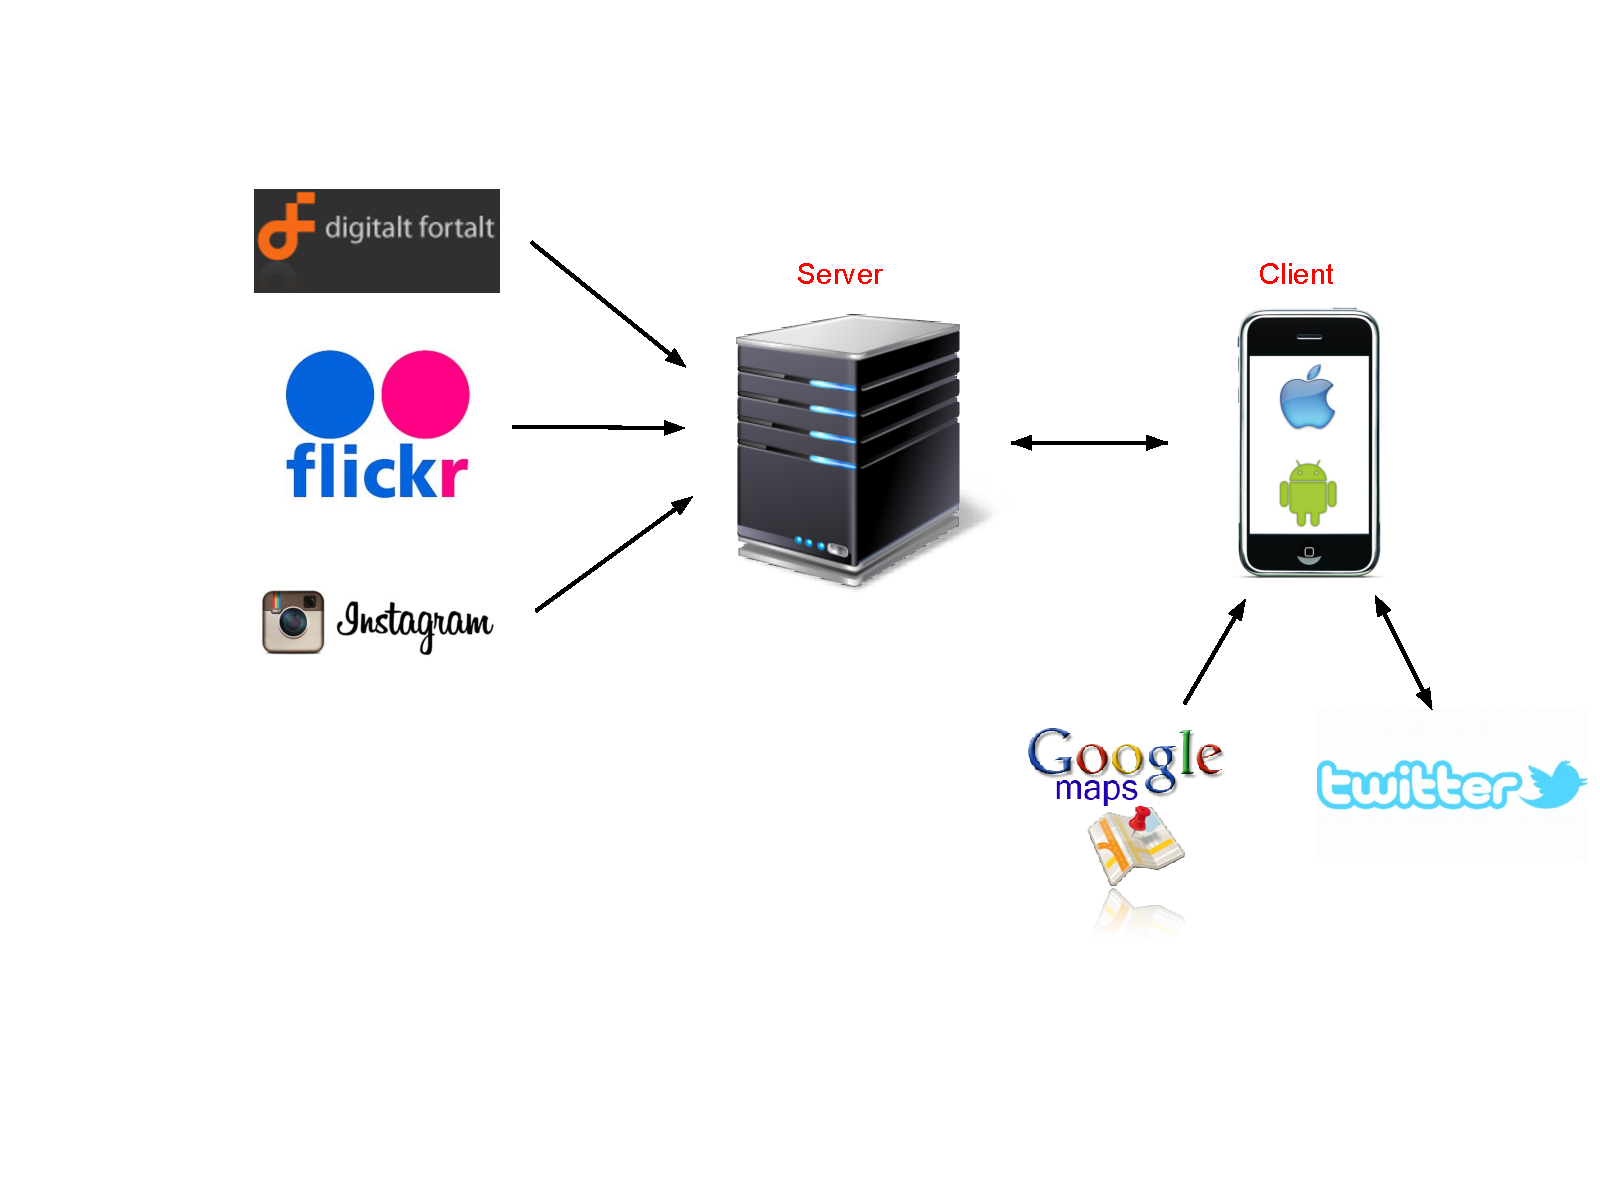
\includegraphics[scale=0.45]{ntoverview-architecture}
\caption{A simple overview of the architecture}
\end{center}
\end{figure}

\begin{itemize}
\item Browse a map and zoom in and out.
\item Load \textbf{places}.
\item Click on a place in the map and access \textbf{stories} from Digitalt Fortalt.
\item Get social media related to a place from the content providers Instagram and Twitter.
\item Go to a users exact position on a map.
\item Search for a location in the map.
\end{itemize}
	
		\subsubsection{Limitations}
There are some limitations to the system that needs to be further developed, and some that probably would require total architectural review of the project to be fixed. Our task is to continue the development of the application. An overview of the features we are going to improve are discussed in the requirements section \ref{sec:Reqs}. 

		\subsubsection{App evaluation}
		
After the first meetings we concluded that the best way to proceed is to evaluate the existing system, to uncover potential issues and flaws.
Therefore we decided that everyone should individually do a usability test when exploring the app for the first time. Here is a short summary of all our reports:

The first major issue most of us experienced is how slow the app loads, with no feedback that something is actually working in the background. Another thought that generally comes to mind is \emph{I don't understand the apps function when opening it without prior knowledge}. What happens is that you get a map with tags you could click on, making you believe the function of the app is to use it when visiting a town (not Trondheim in particular) and want to explore historical monuments and get Wikipedia facts. When clicking on tags you get to the location-specific page, with content from Instagram. Some of us found this social feature not to have very obvious intentions. The social integration seemed out of place. You would want actual and useful information about places to be displayed first. One could also get confused when suddenly a lot of Instagram photos with random people suddenly appear. Our first impression is that this social aspect have to offer something more interesting to be relevant at this stage. 
\\
There is a nice touch with a slight gradient in the bottom indicating that you can scroll down for more content. When the phone is turned (switched to landscape mode) there are issues however. There is no scroll function here limiting the content available and the images are cropped. Also, if there is a lot of text added in the Instagram feed, it disappears along with the hash-tags. The way to collect images from Instagram to the application also seems to be sub optimal when irrelevant content are displayed. When tweeting there are no limitations on length, which causes problems when trying to post tweets over 140 characters.\\
\\
These are some of the feedback extracted from the individual tests. 

		
	\subsection{Survey}


	One of the most important research we did during the pre-study was to conduct interviews about Stedr. In these interviews we let six everyday people, use the current version of Stedr and paid close attention to how they used it. The subjects was both male and female raging between 18-30 in age. The main purpose of this interview session was to get feedback on proposed features from our customer.\\*[8pt]
	Firstly, after the test subject had some time to play with the app. We asked asked some questions about social media integrations, and this is the results:\\

	\emph{Can you see yourself tweeting about a place from Stedr?}\\
	Yes: \textbf{0}\hspace{0.5cm}
	No: \textbf{3}\hspace{0.5cm}
	Don't know: \textbf{3}\\[6pt]
	
	\emph{What about Instagram?}\\
	Yes: \textbf{0}\hspace{0.5cm}
	No: \textbf{3}\hspace{0.5cm}
	Don't know: \textbf{3}\\[6pt]
	
	\emph{What about SoundCloud?}\\
	Yes: \textbf{0}\hspace{0.5cm}
	No: \textbf{4}\hspace{0.5cm}
	Don't know: \textbf{2}\hspace{0.5cm}\\[6pt]

	Additionally, we asked about Wikipedia. This was a proposition from us.\\*[8pt]
	\emph{Would you like the app better if Wikipedia was integrated?}\\
	Yes: \textbf{6}\hspace{0.5cm}
	No: \textbf{0}\hspace{0.5cm}
	Don't know:  \textbf{0}\\*[8pt]
	In retrospect, we see that even though people were positive to this, it doesn't really fit into what Stedr is about. Because of this, we abounded this feature late on.\\
	
	When asked if they can envision using the app in the future, this was their responses:
\begin{itemize}
	\item ”Yes, if the app can also show patios.”
	\item ”Unfortunately, I don't use social media that much, but if the app was more historically oriented, I would be intrigued to use it.”
	\item ”Yes totally!”
	\item ”It must be better than Google Maps for me to bother using it. I want the social features, but only for contributing, not for looking at what other people write. I would also use twitter with the app, but only if there was pre defined tweets.”
	\item”Maybe, if I knew about it.”
	\item ”Yes, it sounds like a good idea.”
\end{itemize}

	The general consensus was very positive about Stedr. Everyone liked the idea, but some were sceptical in regards to the social features that was purposed.

	In response to these results, our customer thought this survey was interesting, but it did not change her mind about trying out these features, in part because she had previously organized focus groups with other results. We respect this decision of course, but feel that it was right of us to do this research regardless.
	
	\subsection{Tools and technologies}
	
		\subsubsection{APIs}
		

		There was a wish from the customer that we should use other existing services as mush as possible instead of having our own database and a comprehensive back-end. The result of this is that the project will be dependent on many different APIs to function properly. As a result of this we spent a lot of time researching different APIs. The existing system had already Norvegiana, Flickr, Instagram and Twitter, though some of them needed a fresh up. In addition, our customer had ideas to expand functionality which meant more APIs. We did research on a lot of different APIs like Google Places, Wikipedia, NRK but did not end up using any of them after consulting with our customer. 
		
\paragraph{Digitalt Fortalt and Norvegiana.}

After a evaluation in the pre-study phase we decided to switch the main API of application for better performance. Here is a short summary of why:

In current condition, Stedr uses an API called Norvegiana. This API is basically a collection of all public APIs that can be used in collecting different data. The major pros using Norvegiana is the portion of information accessible from different sources including \emph{Statsarkivet, Digitalt Fortalt, Digitalt Museum} etc. There are many filtering options making Norvegiana able to return all the information needed.

There has been some complaints about how the current service works. Norvegiana is an interface to the dissemination system, not the production system. Which means that when a story is created, one has to wait for the Art Council Norway to perform an export from production to dissemination. This means that stories are not available through Norvegiana at once after they are produced. In some case we had to wait a few weeks. This is not acceptable with respect to our goal of increasing user participation and enhancing usability. We think this problem might be solved by switching completely to the Digitalt Fortalt API, which should not be too much trouble considering the existing code only makes simple calls to the API trough Norvegiana. It is worth noting that Digitalt Fortalt is originally meant for Norwegian cultural heritage, which might cause problems in a potential international expansion.

The functionality in the APIs, for our usage, are about the same. Where both come short is that both strictly speaking work like databases that you only can retrieve information from, making them impossible to use for posting new content. This has to be solved in another way.

	\subsection{Similar products}
		
As a part of this project we have reviewed apps that come close to our own in regards to purpose, target groups and functionality. One of the apps we looked at is Trondheim Guide.

One of the best features of Trondheim Guide is virtual reality, where you can look into the screen and see what you have in front of you. This can for instance be used to see the distance to the nearest cultural heritage or attractions. You can also have your own journal, where you can add places you have been to. This is tracked with time and date. There is also an very nice feature where you can make your own postcard, and share it with friends. For each place you visit you can check in with both comments and picture, this is saved in your log as well. Although Trondheim Guide is first and foremost an tourist app, it can also be used to discover various cultural heritages around Trondheim.

Another app that overlaps a lot with ours is KNappen. KNappen is an aesthetically pleasing, well-designed app with a user-friendly GUI. Like our own app it is focused around places. You will find images, routes, augmented reality, audio, video and informative and historical texts related to places. Users can also see the Wikipedia article about the place and they can see related places. They have a map view that is somewhat similar the one in our app, where icons are used to represent the different places.


\begin{figure}[h!]
\begin{center}
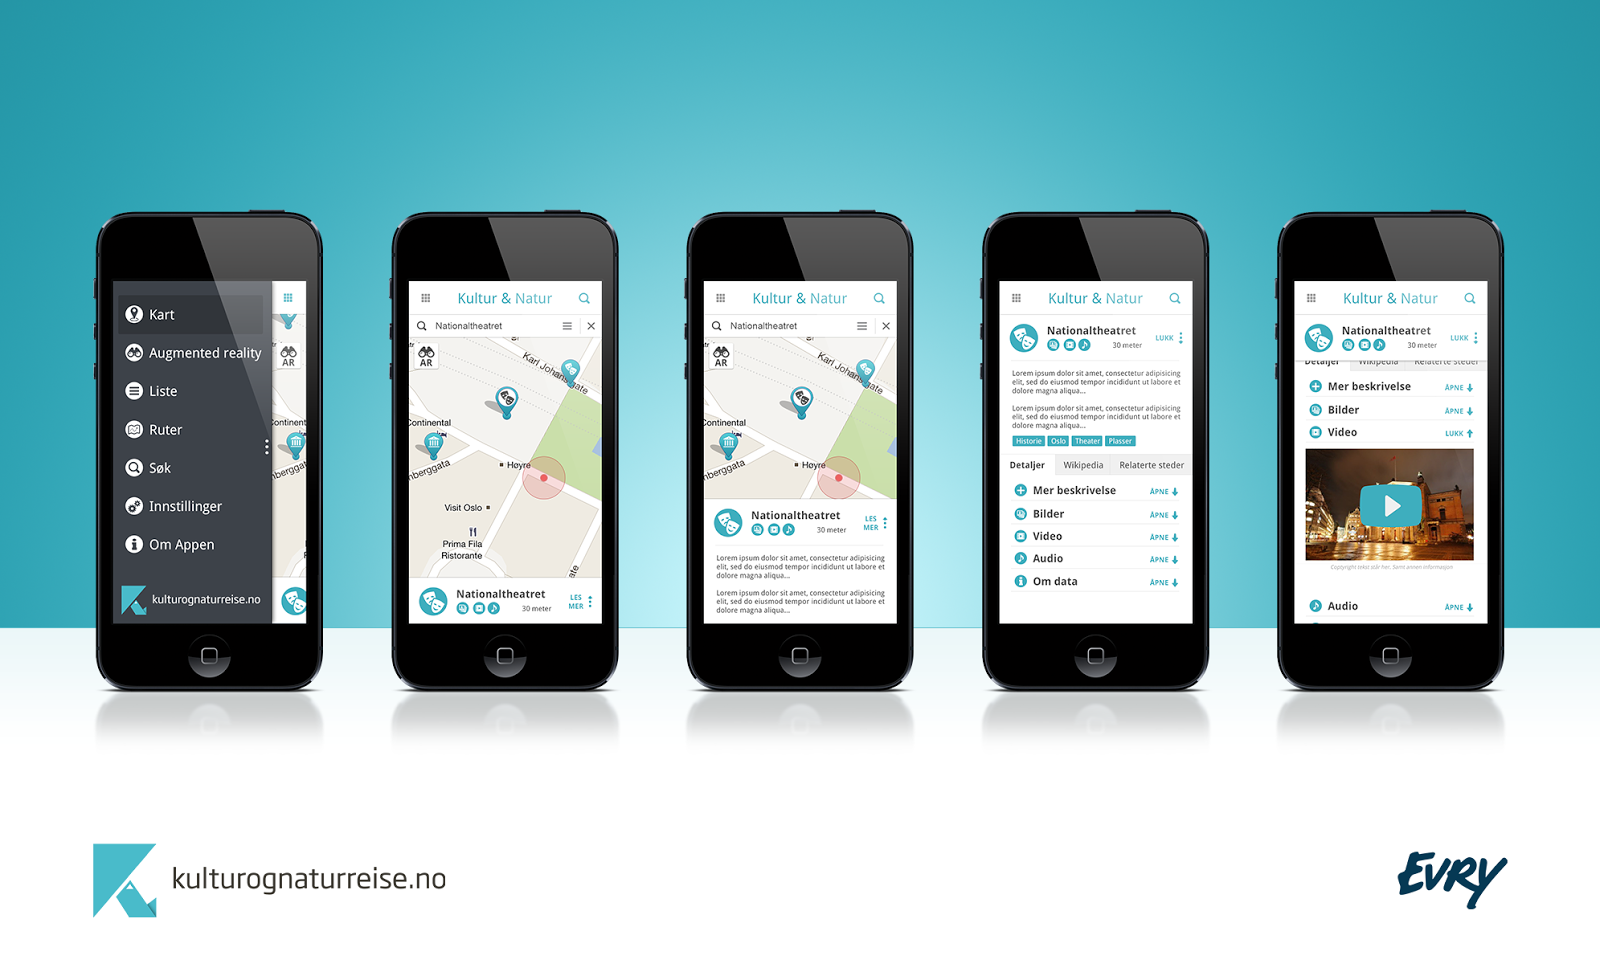
\includegraphics[width=1\textwidth]{res/image02.png}
\caption{KNappen screenshots}
\end{center}
\end{figure}


We think Stedr could benefit from implementing some of the features from these two apps. Especially virtual reality from Trondheim Guide would be a great addition to the app. The user experience from KNappen is also something Stedr could take some inspiration from

\section{Project organization}
\thispagestyle{plain}
	\subsection{Responsibility Areas}

Good delegation of responsibilities helps so that someone at all times have an overview over what tasks needs to be done in specific areas. This also makes it easier to estimate workloads and delegate tasks during the group meetings. It is important to note that even though there are specific responsibility areas, all the group members will be able to get practical experience in all of the project areas, even though the time spent in different areas will be distributed individually according to the responsobility areas.

\begin{description}
\item[Øyvind Hellenes - Scrummaster] Øyvind was selected as the scrum master because of his leadership qualities and because he early on took an interest in the organizatorial part of the project.
\item[Jon-André Brurberg - Project leader] Jon-André is the driving force in this team and hence, he is also the project leader. Additionally, Jon Andre showed interest in the documentation so he is also responsible for this.
\item[Tor Økland Barstad - Technical coordinator] Tor, with his compentance and knowledge of programming, is our technical coordinator and will thus oversee the code and functions as a technical supervisor for the group.
\item[Jørgen Rugelsjøen Wikdahl - Testing manager] Jørgen is responsible for testing the application to make sure the application has as few bugs as possible.
\item[Hallvard Jore Christensen - Report coordinator] Hallvard have the main responsibility of managing the report. This is because of his experience with \LaTeX and report documentationin in general.
\item[Vegard Storm - Usability manager] Vegard showed interest in making sure the application is as user friendly as possible and will manage that aspect of the project.
\end{description}
	
	\subsection{Process model}
For the process model we chose to use the Scrum framework. This was the most natural choice for us amongst the agile methods since it’s a system we all have experience with through previous projects. There are many advantages working with Scrum. It gives clear priority for features and deadlines, which will allow us to focus more of our energy on other vital tasks. This approach promotes communication and transparency. All the team members as well as the client always knows what’s going on and the current tasks’ development through the product backlog. With the backlog cards, the whole production team is also involved with the overall time estimate, which makes it fairly accurate and controllable.

We considered a few other methods as well, like kanban and XP, but came to the conclusion that Scrum was the system for us. This was due to Scrums many structured rules which brings order, but still allows us the freedom we might need during the projects development.

With Scrum we’ll work in iterations called “Sprints” which are typically a week or two, we also stibe towards making these sprints incremental. Doing this, the model is designed, implemented and tested incrementally, feature by feature, until the project is finished. The advantage here is that for every sprint we have a working product to show for, which is a good referance to have, both for ourselves and the customer. 

Since we already have a working project from the very beginning for us to further develop, there is some obvious phase partitions. The first consists mainly on assessing the current version of the product and define the path ahead before we start the actual programming. This will be done through thorough dialog and discussion with SINTEF, to give us a unison idea of where the product are heading. User evaluation is also important in this phase, both internally and externally within the target user group. And of course technology and framework selection. After this comprehensive planning, the actual coding phase can begin. The sprints will be a big part of this, and since we are working incrementally; So we will do with the testing. Following this: the evaluating phase. In which user tests hopefully will force as many problems and bugs with the early version to surface, for us to correct.

Prototypes through a digital mock-up will be important in the planning phase. We have chosen to use Balsamiq for this, which will mean we’ll have an interactive prototype mock-up to show the customer, and should also make sure we're all on the same page. This makes it easier to have something concrete/”physical” as a reference.

\subsection{Development Environment}

Since our project is based on further developing on an existing product, there’s an advantage in using the same main framework as the previous developers. We decided to use Titanium to easily develop a multi-platform app, but we also took a close look at other options (like phonegap) and compared them meticulously in their most critical aspects. With the Titanium framework we use the Titanium SDK which is based on eclipse but tailored for it. For sharing code, Git was our system of choice, mainly because we were already familiar with it, and know it has all the functionality we could need throughout the project. Other documents and files, like notes, summaries, etc. we decided to share through a dedicated Google Drive and Dropbox folder, because each has its own advantages in different aspects. As SCRUM service we first choose Agilefant, but later decided to just use spreadsheets instead.

This project obviously involves working with a big set of APIs, like social media, dictionary and other media services. These’ll play a great part of the development and introduce other frameworks we’ll have to account for. For communication we often use mail and chat-services, but we prefer more “personal” forms of communication like a video chat through skype, phone calls and/or ideally, meetings in person.

\subsection{Work Breakdown Structure}
This Work Breakdown Structure is an overview of what we have done and how our work is distributed between packages. It is updated to match our end result.
We have given percentages to each task to show how much work have been put into it.

\begin{figure}[h!]
\begin{center}
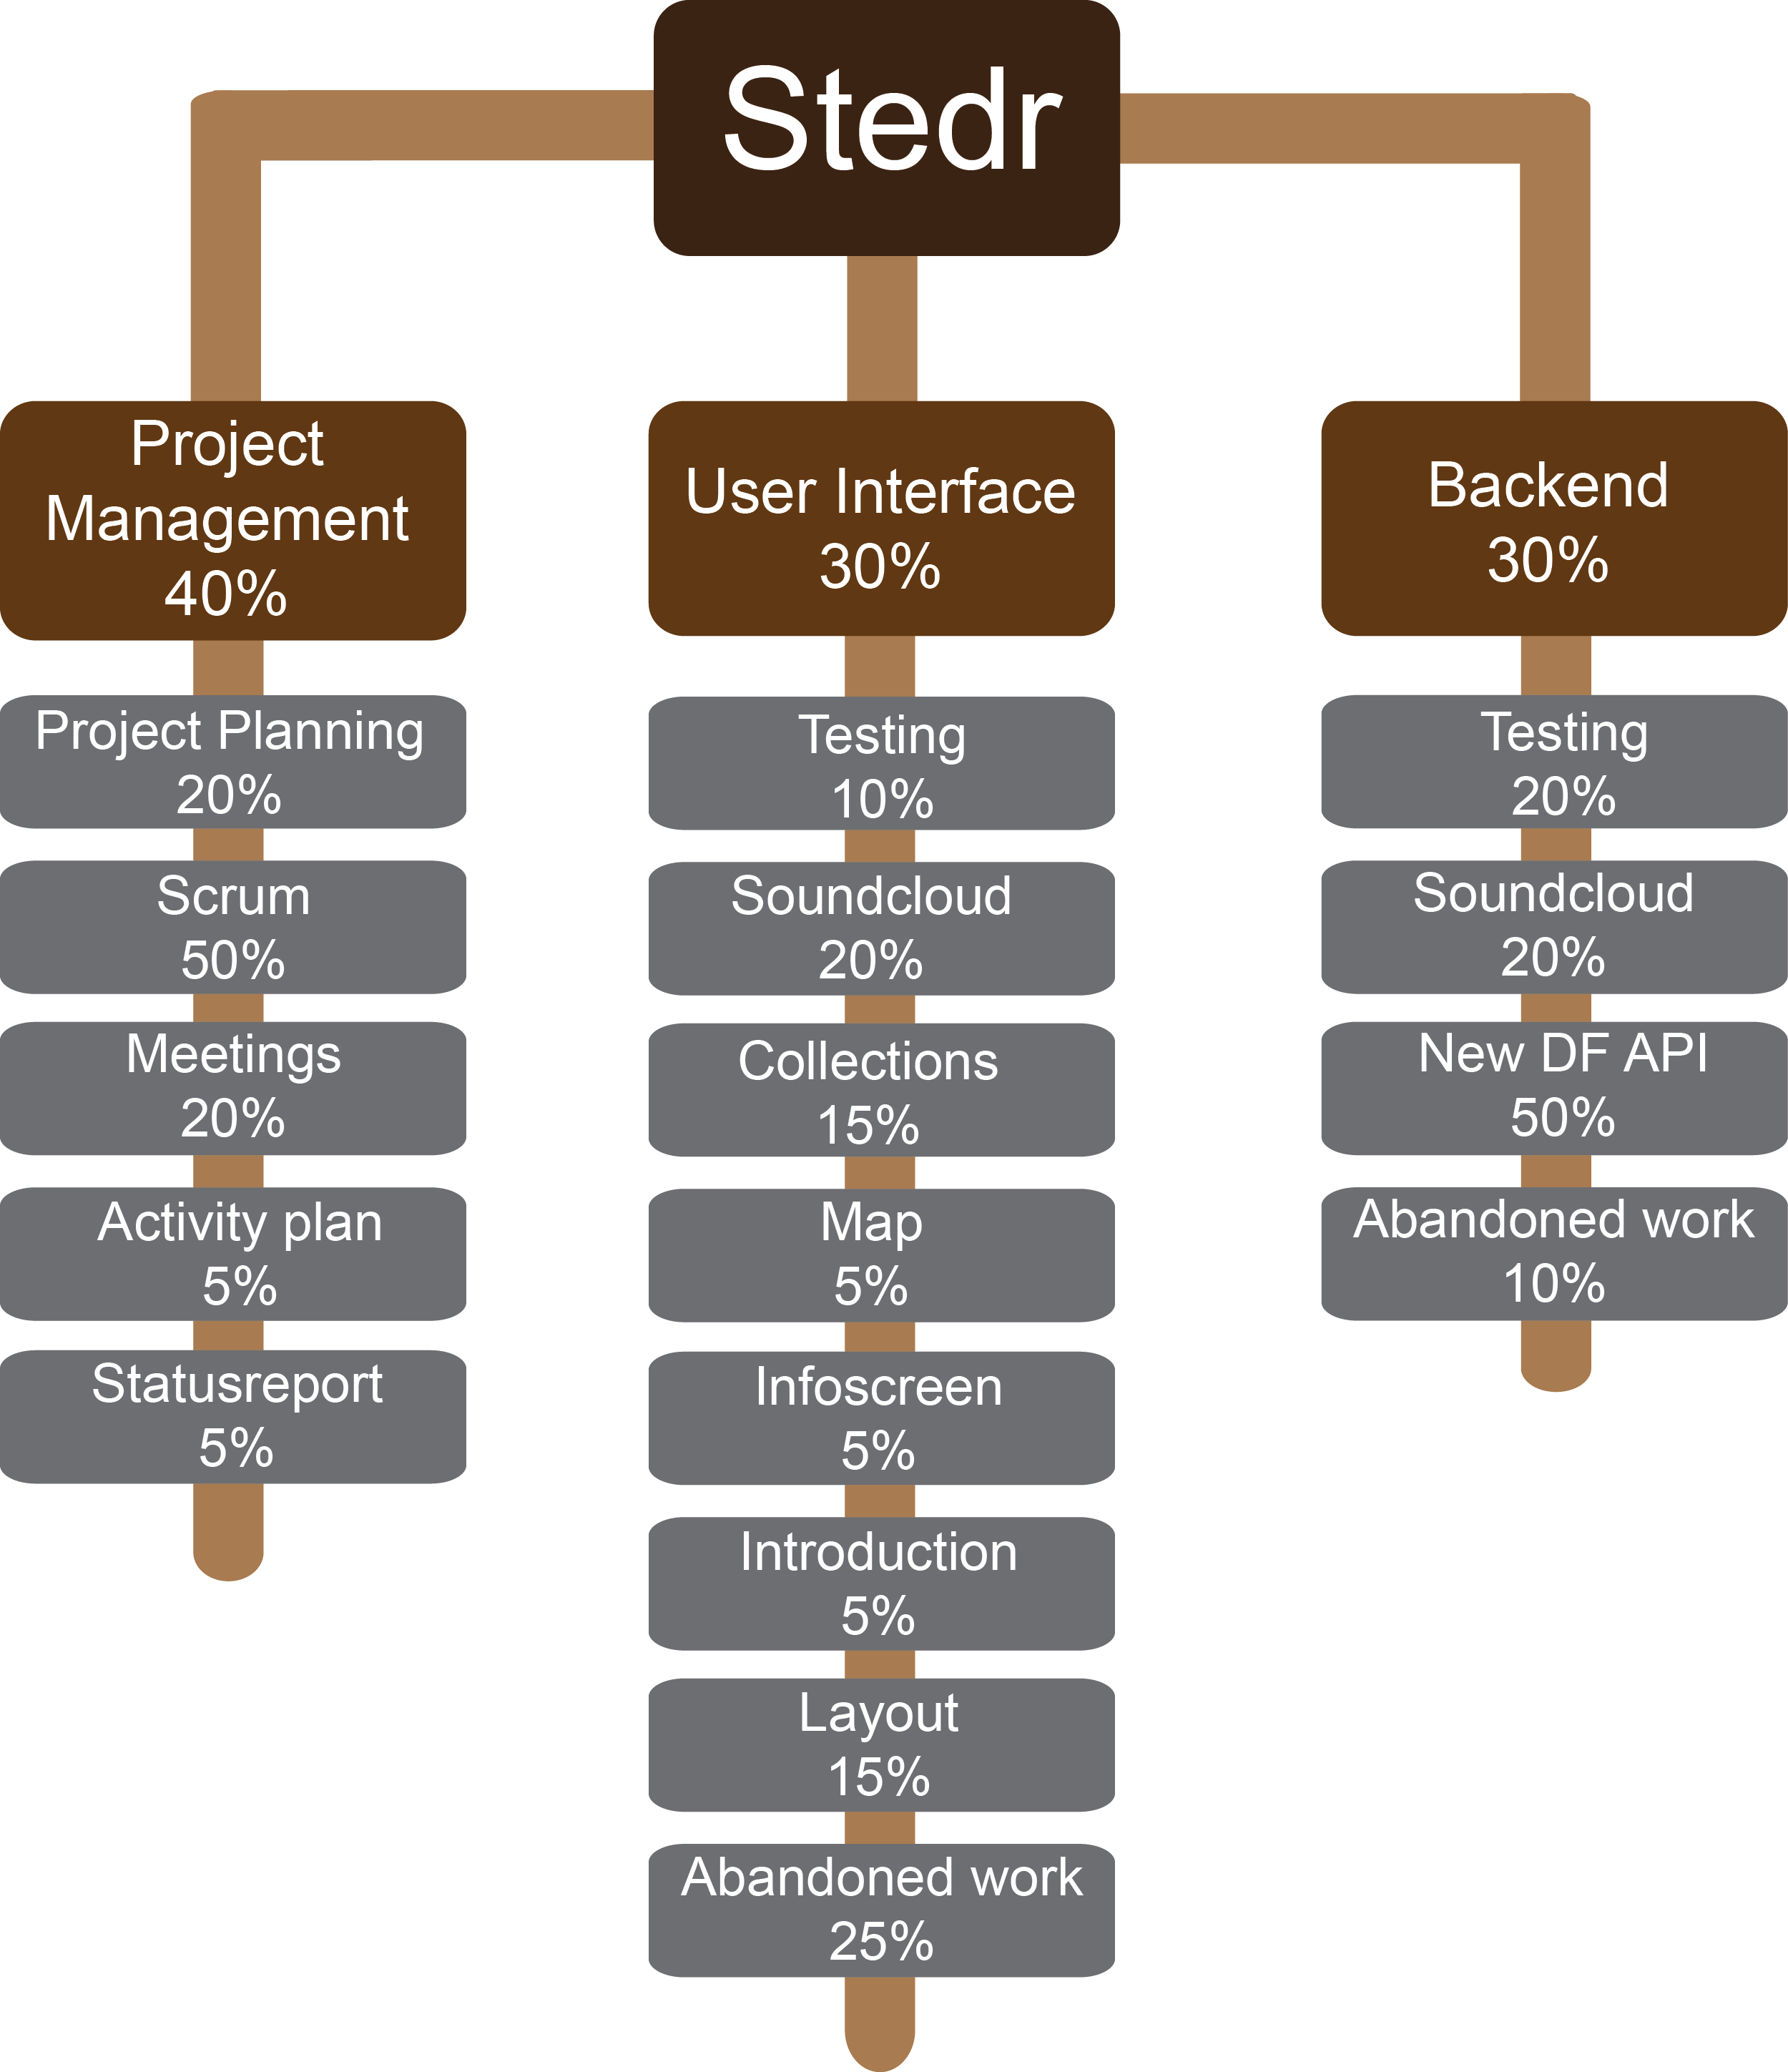
\includegraphics[scale=0.6]{WBS}
\caption{Work Breakdown Structure}
\end{center}
\end{figure}
\clearpage

\subsection{Project Planning}



\clearpage
\section{System Requirements Specification}

\subsection{Purpose}
This is the software requirement specification for the new version of Stedr, both the backend system that provides content and also the frontend that shows the content and the context of the content to the user. Here the traditional architectural terms backend - and frontend are used, but there are some subtleties to this term, as the frontend itself is managing a content service of its own. 

\subsection{Intended audience and reading suggestions}
Intended readers for this document are current and future developers, and the customer. The reader should also be noted that the SRS both can be read as a stand-alone document to get an overview of the rationalization behind the development process, but that it also is a part of the project report as a whole


\subsection{References}
The software requirements are based on the standard as provided by ISO/IEC:25010 \cite[10]{25010}, and also the models that can be found in this report’s section for architecture and modelling. References to the ISO-standard and other literature are found at the end of the project report under references.

\subsection{Product perspective}
Originally Stedr is a product developed by students at NTNU as a part of the subject TDT4290, and this application will form a basis for out continued development. The state of the exisiting application is considered to be a working prototype, and to some degrees it is an application that is built up with a traditonal server-client architecture. A simple technical overview of the system is provided below. 

\begin{figure}[h!]
\begin{center}
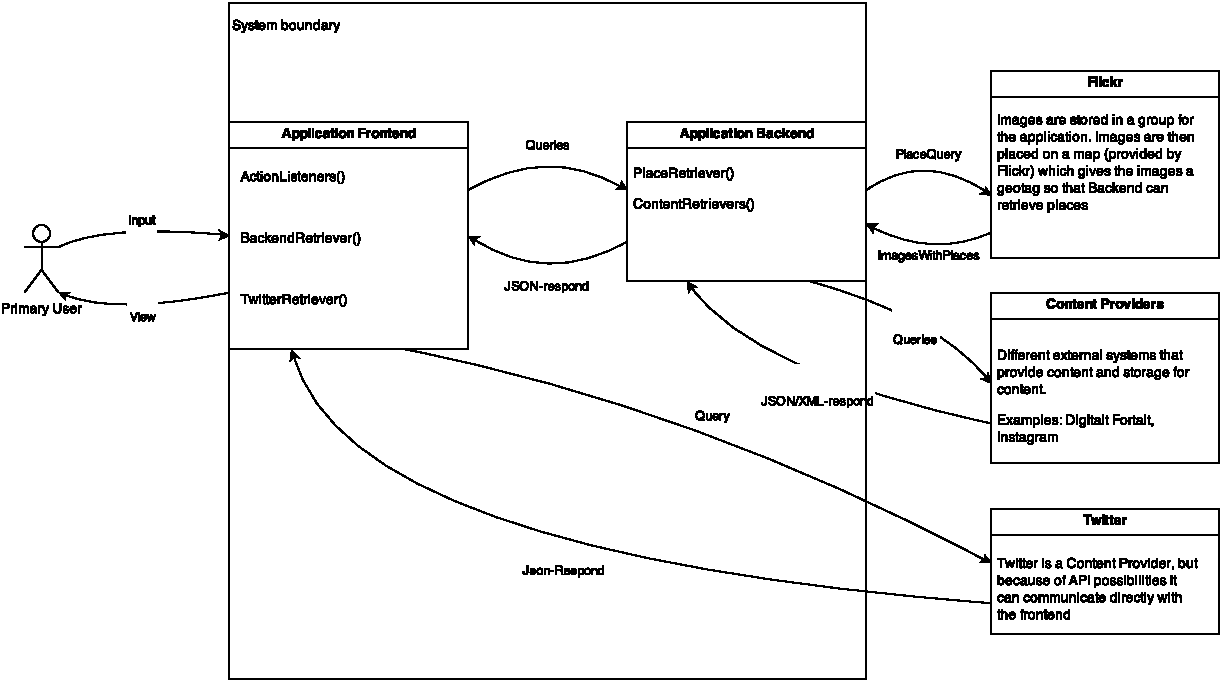
\includegraphics[scale=0.6]{tooverview-architecture}
\caption{A simple technical overview of the architecture}
\end{center}
\end{figure}

\subsection{User classes and charateristics}
The users of the program mainly divide into two categories. One is the primary user group which are using the frontend to see content. A typical user of this sort is a highschool student which is introduced to the program in the context of cultural heritage awareness. Most of these student will likely not use the program outside of the school context, but there is a possiblity that some of these students transits to the second category. Under the second category there are two user types, one is the content providers and the other is the maintainer. 
(See another section)

\subsection{Operating environment}
The frontend application of the system is a mobile application which aims to run on both the Android and iOS platform. Because of difficulties with developing towards the iOS platform without equipment from Apple, it's still discussed how the system is going to be tested on iOS. The backend of the server running as a server application, provided by Heroku.


\subsection{Product functions}

\subsection{Design and Implementation Constraints}

\subsection{User Documentation}

\subsection{Assumptions and Dependencies}
 
\subsection{External Interface Requirements}

\subsection{User Interfaces}
 
\subsection{Hardware Interfaces}
 
\subsection{Software Interfaces}

\subsection{System Features}

\clearpage

\begin{table}[!ht]
\begin{center}
\begin{tabular}{i{4cm}|| i{10cm}} \toprule

\multicolumn{2}{c}{\textbf{SF-1}} \\ \hline

Name & Find place on map \\ \hline
Priority & H \\ \hline
Goal & To browse the map to find a given place \\ \hline
Actors & Primary User \\ \hline
Preconditions & \begin{enumerate}  \item The home screen is displayes  \item The internal system and external systems are running \item The device has a internet connection  \end{enumerate} \\ \hline
Stimulus-Response  &  \begin{enumerate}  \item The home screen is displayes  \item The internal system and external systems are running \item The device has a internet connection  \end{enumerate} \\ \hline
Alternate Flow & \begin{itemize} \item[2a] The place does not exist and is not shown on the map \end{itemize} \\ \hline
Functional Requirement & A user should be able to access and browse a map, with places as pinpoints at their respective geographical location. The pinpoints should contain the picture and information found on Flickr. Group places close to eachother in one icon on map. \\ \hline
Related Use Cases & 1,3 \\ \hline
Dependencies & none \\ \bottomrule

\end{tabular}
\end{center}
\end{table}

\begin{center}
\begin{tabular}{i{4cm}|| i{10cm}} \toprule

\multicolumn{2}{c}{\textbf{SF-2}} \\ \hline

Name & Open menu \\ \hline
Priority & H \\ \hline
Goal & Open the drawer menu  \\ \hline
Actors & Primary User \\ \hline
Preconditions & \begin{enumerate} \item 2,3 \item[4] A screen with the menu button \end{enumerate} \\ \hline
Stimulus-Response & \begin{enumerate} \item The user clicks the menu button \item The menu opens \end{enumerate} \\ \hline
Alternate Flow & \begin{itemize} \item[1a] The user clicks the menu button, and the menu is already open \item[2a] The menu closes \end{itemize} \\ \hline
Functional Requirement & A button with the possibility to open the menu should always be presented to the user, so that the user easily can navigate the application. \\ \hline
Related Use Cases & 1,2 \\ \hline
Dependencies & none \\ \bottomrule

\end{tabular}
\end{center}

\begin{center}
\begin{tabular}{i{4cm}|| i{10cm}} \toprule

\multicolumn{2}{c}{\textbf{SF-3}} \\ \hline

Name & Search for a location \\ \hline
Priority & M \\ \hline
Goal & Go to a location on the map \\ \hline
Actors & Primary User \\ \hline
Preconditions & \begin{enumerate} \item 1,2,3 \end{enumerate} \\ \hline
Stimulus-Response & \begin{enumerate} \item The user searches for a location with the search bar in the map view. \item The map navigates to the location \end{enumerate} \\ \hline
Alternate Flow & \begin{itemize} \item[2a] Location is not found and is not navigated to. \end{itemize} \\ \hline
Functional Requirement & A search bar related to the map should be presented to the user, so the user can search for locations (independent of places) to see if there are any stories at that place. \\ \hline
Related Use Cases & 1 \\ \hline
Dependencies & none \\ \bottomrule

\end{tabular}
\end{center}

\begin{center}
\begin{tabular}{i{4cm}|| i{10cm}} \toprule

\multicolumn{2}{c}{\textbf{SF-4}} \\ \hline

Name & Refresh map \\ \hline
Priority & H \\ \hline
Goal & Update the map with content. \\ \hline
Actors & Primary User \\ \hline
Preconditions & \begin{enumerate} \item 1,2,3 \end{enumerate} \\ \hline
Stimulus-Response & \begin{enumerate} \item The user clicks the update button. \item The map refreshes and show new places \end{enumerate} \\ \hline
Alternate Flow & \begin{itemize} \item[2a] No new places are found, so no places are added to the map. \end{itemize} \\ \hline
Functional Requirement & The user should be presented with a button that makes requests for new places with content when pushed. This function should also be done automatically so that new content is sent to the user within 5 minutes after it’s added. \\ \hline
Related Use Cases & 1 \\ \hline
Dependencies & none \\ \bottomrule

\end{tabular}
\end{center}

\begin{center}
\begin{tabular}{i{4cm} ||  i{10cm}} \toprule

\multicolumn{2}{c}{\textbf{SF-5}} \\ \hline

Name & Go to location \\ \hline
Priority & H \\ \hline
Goal & Go to users location. \\ \hline
Actors & Primary User \\ \hline
Preconditions & \begin{enumerate} \item 1,2,3 \end{enumerate} \\ \hline
Stimulus-Response & \begin{enumerate} \item The user clicks the gps button. \item The map zooms to the users location.  \end{enumerate} \\ \hline
Alternate Flow & \begin{itemize} \item[2a] GPS not available so it can’t go to the users location. \end{itemize} \\ \hline
Functional Requirement & Since the user has the possibility to navigate the map freely, it should also be possible to quickly navigate to places relevant (in context of location) to him/her. \\ \hline
Related Use Cases & 1 \\ \hline
Dependencies & none \\ \bottomrule

\end{tabular}
\end{center}

\begin{center}
\begin{tabular}{i{4cm}|| i{10cm}} \toprule

\multicolumn{2}{c}{\textbf{SF-6}} \\ \hline

Name & Open views \\ \hline
Priority & H \\ \hline
Goal & Open views and see the content related to that specific view \\ \hline
Actors & Primary User \\ \hline
Preconditions & \begin{enumerate} \item 1,2,3 \end{enumerate} \\ \hline
Stimulus-Response & \begin{enumerate} \item The user clicks on a view \item The user changes views at will \item Content  \end{enumerate} \\ \hline
Alternate Flow & \begin{itemize} \item[1a] If the user clicks a button for the already chosen view, nothing should happen. \end{itemize} \\ \hline
Functional Requirement & For navigation in the place view, the user should be presented with different buttons (or tabs) so that the user easily can navigate between content and still have an overview of what types of content the application provides. Preview picture gallery when places are grouped together. Add description about place, own vire for sound. Be able to show place location on map from story. Be able to filter stories by tag, author, institution video/no video. preview stories by sound from SoundCloud \\ \hline
Related Use Cases & 3 \\ \hline
Dependencies & none \\ \bottomrule

\end{tabular}
\end{center}

\begin{center}
\begin{tabular}{i{4cm}|| i{10cm}} \toprule

\multicolumn{2}{c}{\textbf{SF-7}} \\ \hline

Name & Load content \\ \hline
Priority & H \\ \hline
Goal & Content is loaded from the external systems \\ \hline
Actors & Internal System \\ \hline
Preconditions & \begin{enumerate} \item 1,2,3 \end{enumerate} \\ \hline
Stimulus-Response & \begin{enumerate} \item Access the server as done in the previous version of the system \item Provide input to the server “placeId=” \item Content is loaded and a JSON-object is replied by the server \end{enumerate} \\ \hline
Alternate Flow & \begin{itemize} \item[1a] If the user clicks a button for the already chosen view, nothing should happen. \end{itemize} \\ \hline
Functional Requirement & The API for DF has to be changed, without changing the behaviour of the response from the server. In additon to this the server will respond with a new container for the audio content. Other content should be handled as normal. Retrieve collectionfrom DF based on hashtag and location.  Retrieve stories in a collection from DF based on tags. Open info retrived from SoundCloud based on hashtags or location. Retrieve information from Instagram based on Hashtags. Be able to get tinyUrls to different content. \\ \hline
Related Use Cases & Null \\ \hline
Dependencies & none \\ \bottomrule

\end{tabular}
\end{center}

\begin{center}
\begin{tabular}{i{4cm}|| i{10cm}} \toprule

\multicolumn{2}{c}{\textbf{SF-8}} \\ \hline

Name & Collection \\ \hline
Priority & H \\ \hline
Goal & Get all places related to a theme. \\ \hline
Actors & Primary User \\ \hline
Preconditions & \begin{enumerate} \item 1,2,3 \end{enumerate} \\ \hline
Stimulus-Response & \begin{enumerate} \item Access the menu bar. \item Click on the Collections-button \item Choose a collection \item Collections view is opened \item Change to map view \item Places related to the collections is shown on map \end{enumerate} \\ \hline
Alternate Flow & \begin{itemize} \item[3a] No Collections are available \end{itemize} \\ \hline
Functional Requirement & A container called Collections are to be implemented. Collections. Allow switching between map-related and collection related funtionallity. Display picture, title and description about a collection. Have a storyListView. Preview stories in collection story list. Open story in collection list. Places on map view with icon for each story in colelction. Preview a place for story on map.\\ \hline
Related Use Cases & 3 \\ \hline
Dependencies & none \\ \bottomrule

\end{tabular}
\end{center}

\begin{center}
\begin{tabular}{i{4cm}|| i{10cm}} \toprule

\multicolumn{2}{c}{\textbf{SF-9}} \\ \hline

Name & Upload content \\ \hline
Priority & M \\ \hline
Goal & Upload content \\ \hline
Actors & Primary User \\ \hline
Preconditions & \begin{enumerate} \item 1,2,3 \item[5] The user has an account at the content provider he or she is trying to upload to.  \item[6] Places related to the collections is shown on map \end{enumerate} \\ \hline
Stimulus-Response & \begin{enumerate} \item Access the tabs for different views \item Click the add-button in the views. \end{enumerate} \\ \hline
Alternate Flow & \begin{itemize} \item[3a] No Collections are available \end{itemize} \\ \hline
Functional Requirement & The user should have the possibility to add content so that. Add picture directly from stedr. ask the user for login-credentials the first time, then store locally for continued access. A similar approach for SoundCloud. Have relevant hashtags copied to clipboard. Be able to comment and like pictures on instagram. \\ \hline
Related Use Cases & Null \\ \hline
Dependencies & none \\ \bottomrule

\end{tabular}
\end{center}

\begin{center}
\begin{tabular}{i{4cm}|| i{10cm}} \toprule

\multicolumn{2}{c}{\textbf{SF-10}} \\ \hline

Name & Get help and info \\ \hline
Priority & H \\ \hline
Goal & Be informed \\ \hline
Actors & Primary User \\ \hline
Preconditions & \begin{enumerate} \item 1,2,3  \end{enumerate} \\ \hline
Stimulus-Response & \begin{enumerate} \item Access the drawer menu \item Click the help button. \item Select the option for what help you need \end{enumerate} \\ \hline
Alternate Flow &  \\ \hline
Functional Requirement & Introduction for first users. Help available at any time.\\ \hline
Related Use Cases & Null \\ \hline
Dependencies & none \\ \bottomrule

\end{tabular}
\end{center}




\subsection{Product Quality}

Guided by ISO:25010, meetings with our supervisor and the feature list given to us by the customer the product qualities that are important for the project is functional suitability, portabilty and maintainability.

\subsubsection{Compatibility}


\subsubsection{Performance Efficiency}
Even though the system isn't a part of a critical operation, the new and improved system will have performance efficiency as an important model of quality. The reasoning behind this is that decreased response time between components in the system is specfically asked for at multiple places in the feature list provided by the customer. 

As of now the time to load new content from the content providers to the application is slow and random. Because of this there are no exact estimation on the time used to pull content from Digitalt Fortalt and Instagram, but the application should use no more than \textit{300 seconds} to pull new content. Unrelated to the goal of performance issue; the user should be informed that the application isn't a real-time application.

Requirements related to resources utilized by the application when performing it's tasks, are already met by the prototype. The new version of the application are bound also bound by these goals. Specifically the backend is bound by the resources provided by the 1x Heroku Cloud Platform. Because of the utilization of the Google Maps API, the resources frontend is limited to the bound given to the application from Google Maps. 

Regarding capacity used by the the application, there should be an improvement. Because the application is to be used on the go where there may not be any WiFi-hotspots, the application should restrain itself to dowload content that is unrelated to where the user is. Because of the varied content types, it is hard to set a defined limit in how much contents (in terms of megabytes) the application should download. The limitations given to the application will therefore be set by the equation: \\ 
\begin{center} 
$\textrm{Bound}=\textrm{Content from Digitalt Fortalt}+5\times\textrm{Content from Twitter}+10\times\textrm{Picture from Flickr}+5\times\textrm{Picture from Instagram}$
\end{center}

\subsubsection{Reliability}
Since the application is going to be online without a team responsible for the technical maintenance, the server should be operative as long as the external content providers are feeding it with content. 

Because of the early versioning of the application, the aspect of maturity is not important for this application. Users of the application are few, and they know what the capabilities of the application is. This means that a user follows a rigid pattern and within that pattern, the probability to execute faults is almost non-existing. Functionality outside that pattern is not supported and thereby it's impossible to execute mistakes.

An important charecteristic of the application is that it has to be available just as often as a professional service. This means that under normal circumstances, the uptime of the backend and front should be 99 \%

Whenever faults are occuring, it is crucial that the backend has implemented services so that it can recover without the need of a maintainer. Because of the relative simplicity of the backend, the server should restart itself within \textit{180 seconds}

\subsubsection{Portability}

It is important to the customer that the application is made available on multiple platform as this is a demand by Tag Cloud. The minimal number of platforms which the product should run on is iOS and Android. 

Following this, the frontend of the application should be written once and compiled down to both the iOS and Android platform. The backend should provide agnostic responses, so that the responses can be handled the same by on Android and iOS devices. 

Because of the early development phase of the application, there is not a requirement to install the application from the normal application providers Google Play and Apple Store. It is enough that it is possible to install the applications on development devices. This also leads to that the application doesn't need to consider replaceability at this point.  




\clearpage 					%This command flushes out all the queued floats waiting to be placed to avoid them being placed inapropriately in another section.
\section{Architecture}
\thispagestyle{plain}

The current architecture of the application is as shown in figure 3 \ref{fig:fig1}. We have a back-end written in Java that retrieves information from services like Digitalt Fortalt, Flickr and Instagram. Digitalt Fortalt is where all the stories are obtained from. Flicker holds all the locations, and the pictures are taken from Instagram based on tags. The information is stored on the server and can now be used by the client, which holds the front-end of the application that is being developed on Appcelerator Titanium, using mainly JavaScript and XML. Twitter is integrated directly into the front-end and does not have to go through the server. In addition, we have also added support for Soundcloud. 

\vspace{0.4in}
\begin{figure}[!h]
\begin{center}
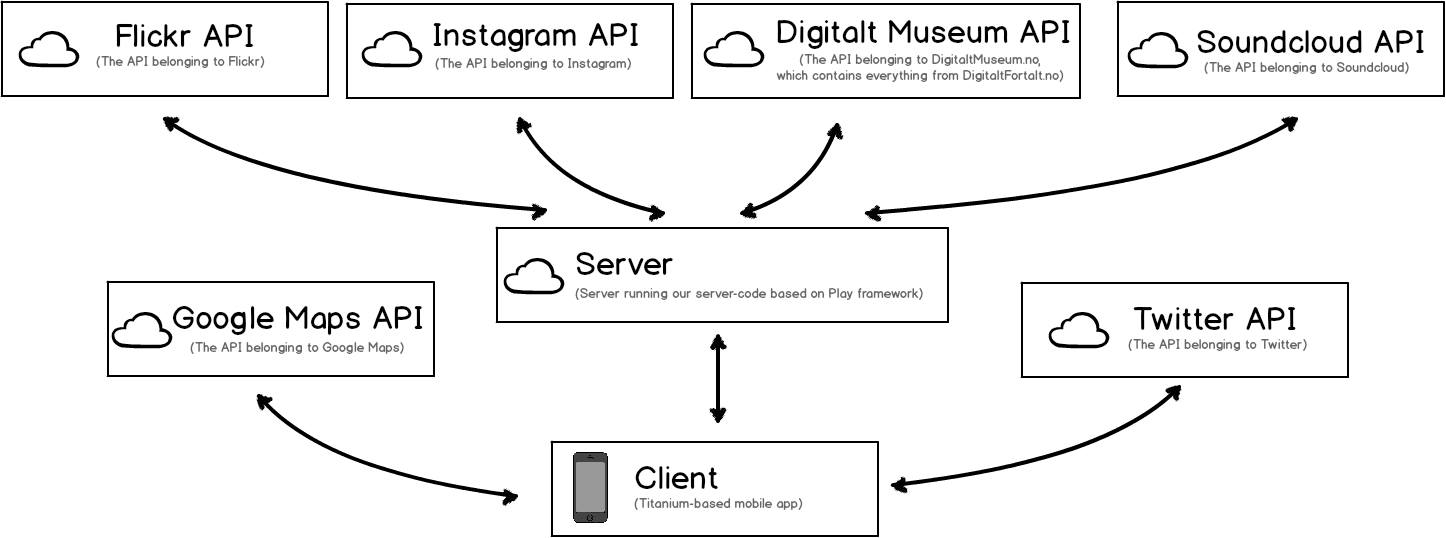
\includegraphics[width=1\textwidth]{res/DeploymentView.jpg}
\caption{Deployment View}
\end{center}
\end{figure}


\subsection{Back-end}
The Back-end is written in Java and mainly retrieves data from external APIs and save it on the server so that it can be used by the application.

\begin{figure}[!h]
\begin{center}
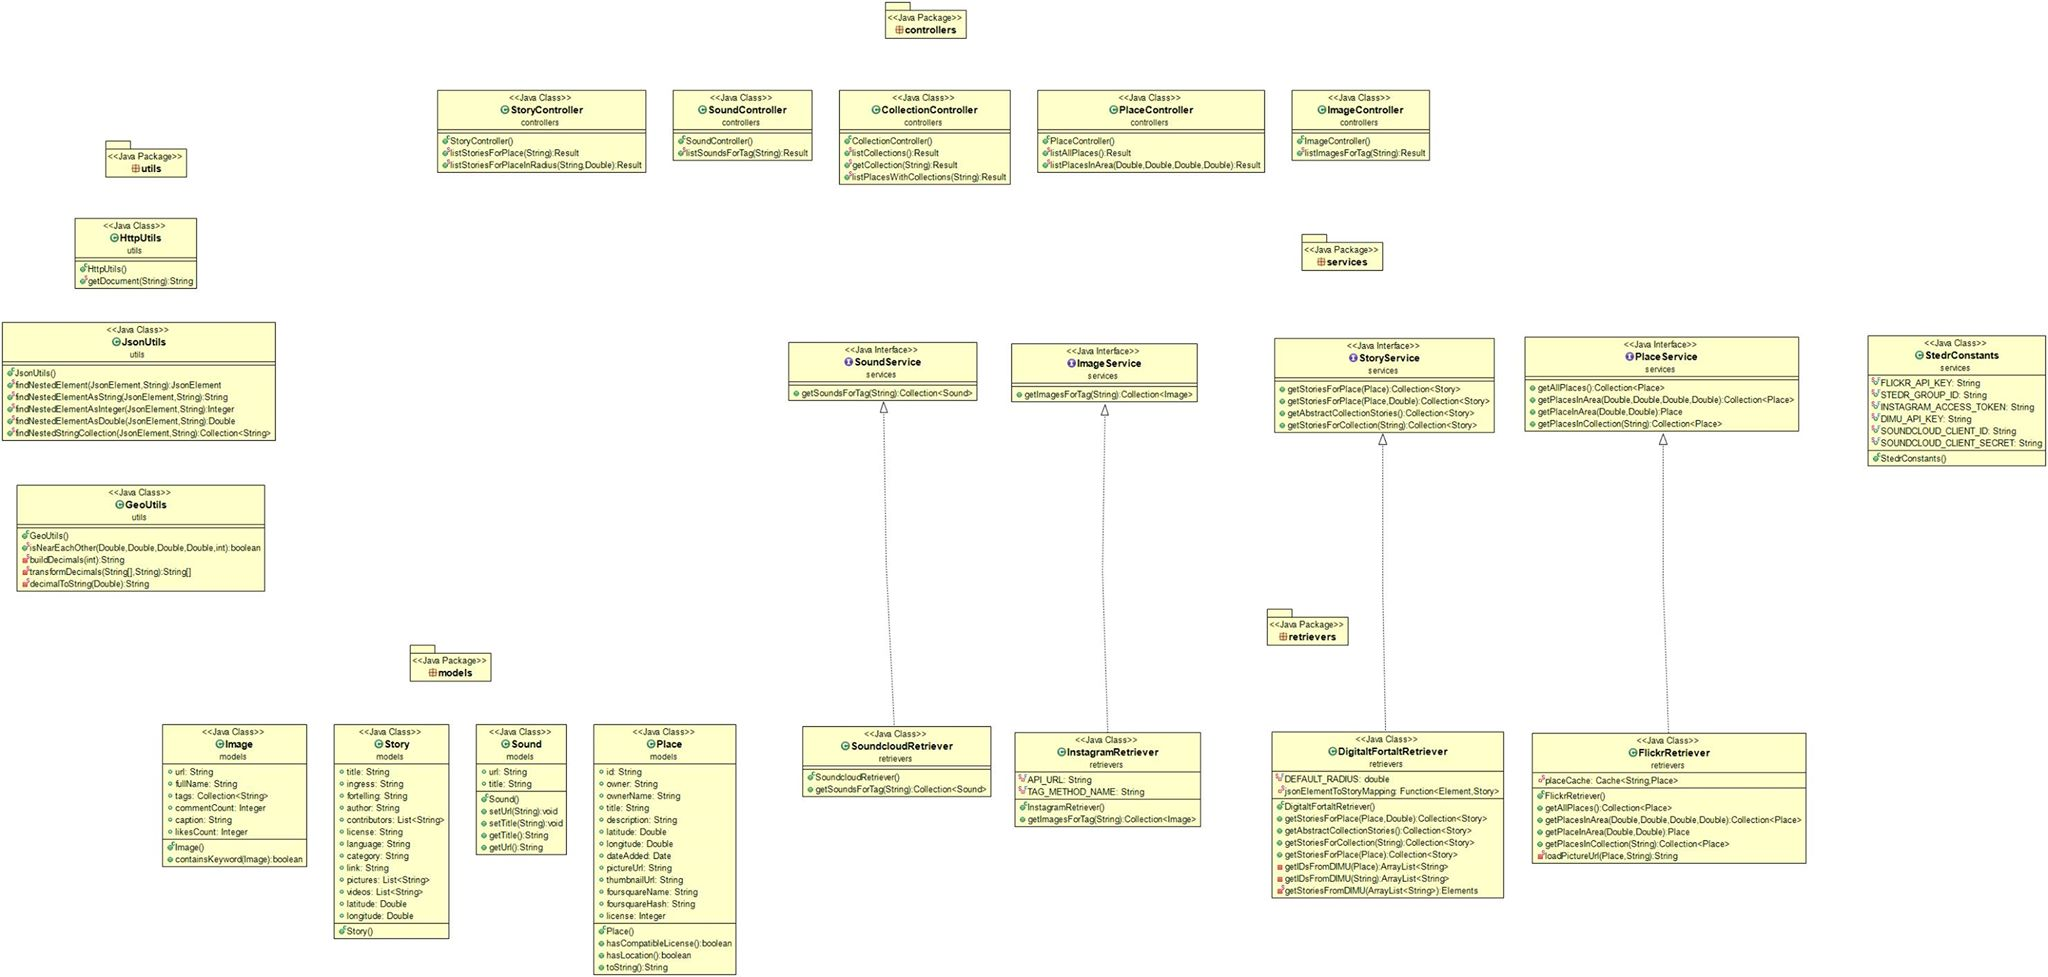
\includegraphics[scale=0.15]{classBack.jpg}
\caption[miniature class diagram: back-end]{Full scale class diagram can be found in Attatchments \ref{sec:classDiagrams}}
\end{center}
\end{figure}

\subsection{Front-end}
The front-end of the application is an interface to let the user enter, manipulate and view data. It is the part of the application that is being interpreted on the users own device, and is based on XML, TSS and JavaScript for design and functionality. 

Every window in the application has a JavaScript-, TSS- and XMLl-file associated with it. A window can contain various views that can each have different event listeners. What the user sees depends on the window currently open and its associated XML, TSS and JavaScript files. What happens when interacting with a view depends on the event-listeners attached to that particular view. Interactions can be purely visual or it can trigger core functionalities. For example the refresh button on the map window has an event-listener attached to it so that when the user clicks it, it will attempt to fetch the locations from the server and plot them on the map. It will also animate the refresh icon to spin, giving the user feedback when the click was registered.


\begin{figure}[!h]
\begin{center}
\begin{tabular}{cc}
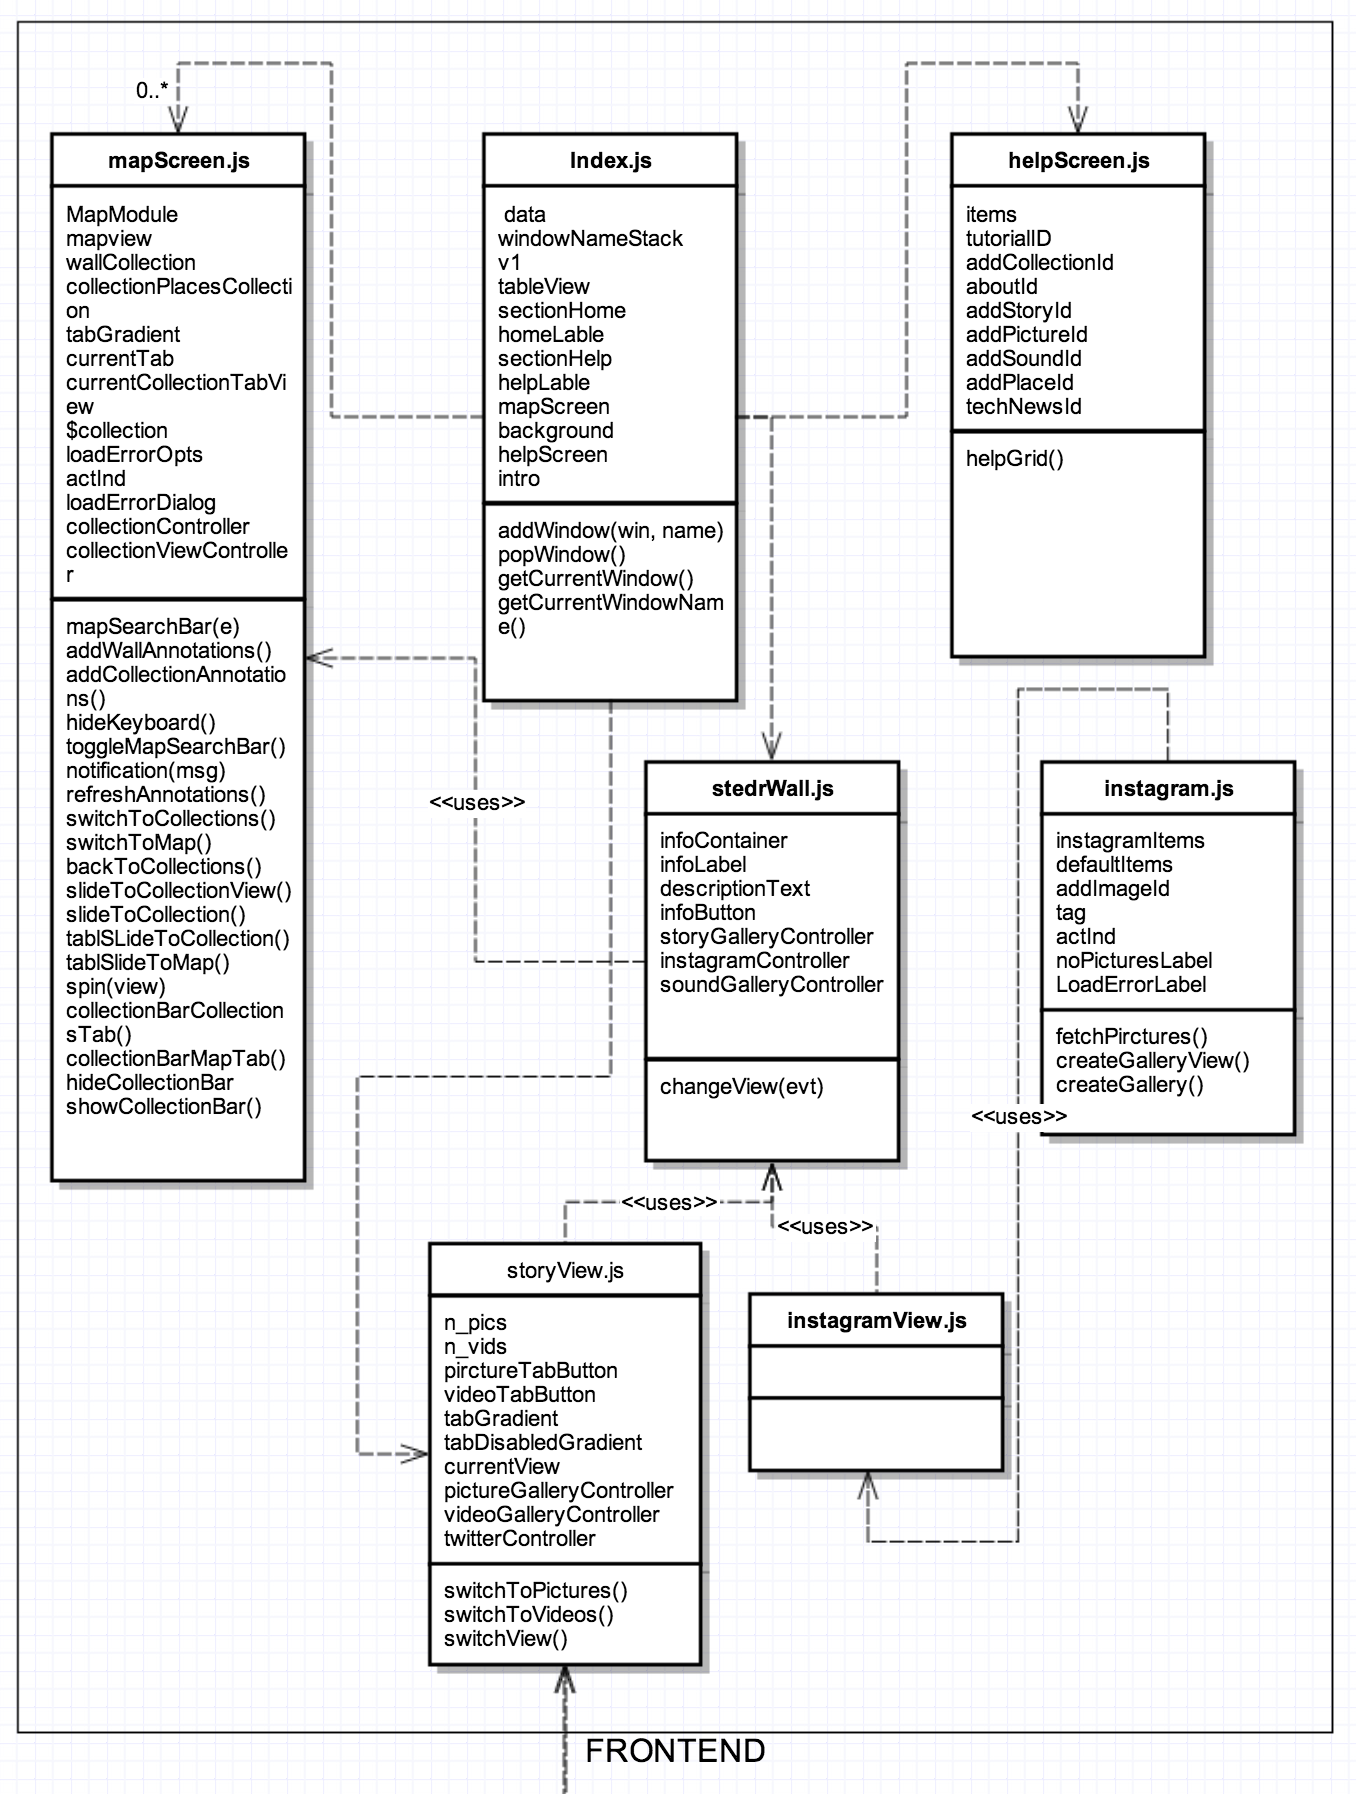
\includegraphics[scale=0.15]{classFront1.png}&
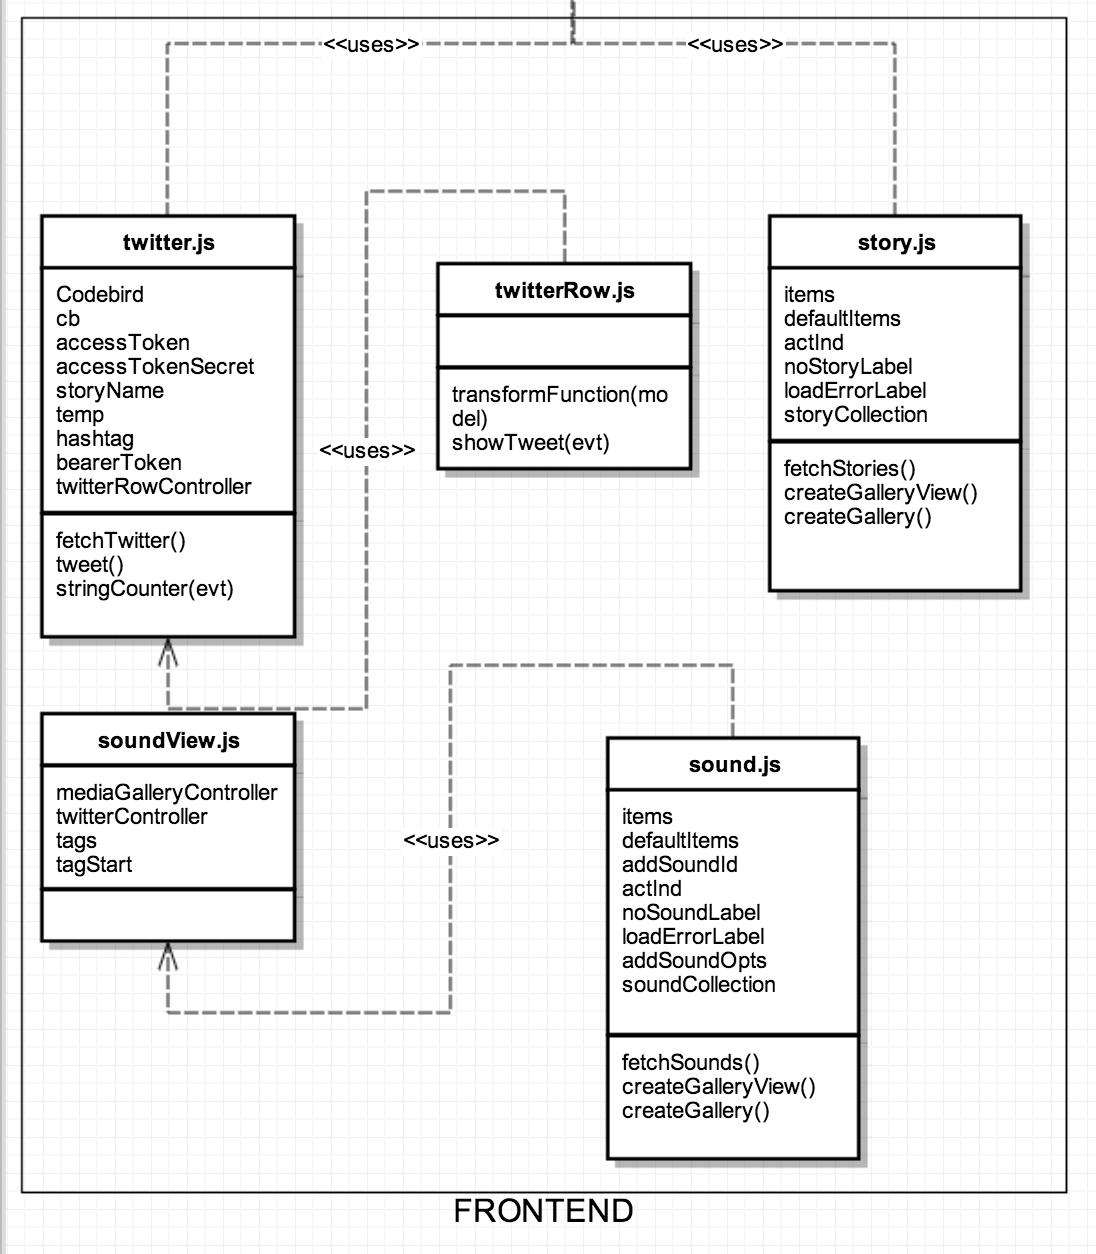
\includegraphics[scale=0.15]{classFront2.png}\\
\end{tabular}
\caption[miniature class diagram: front-end]{Full scale class diagram can be found in Attachments \ref{sec:classDiagrams}}
\end{center}
\end{figure}

\subsection{Process View}

\begin{figure}[!h]
\begin{center}
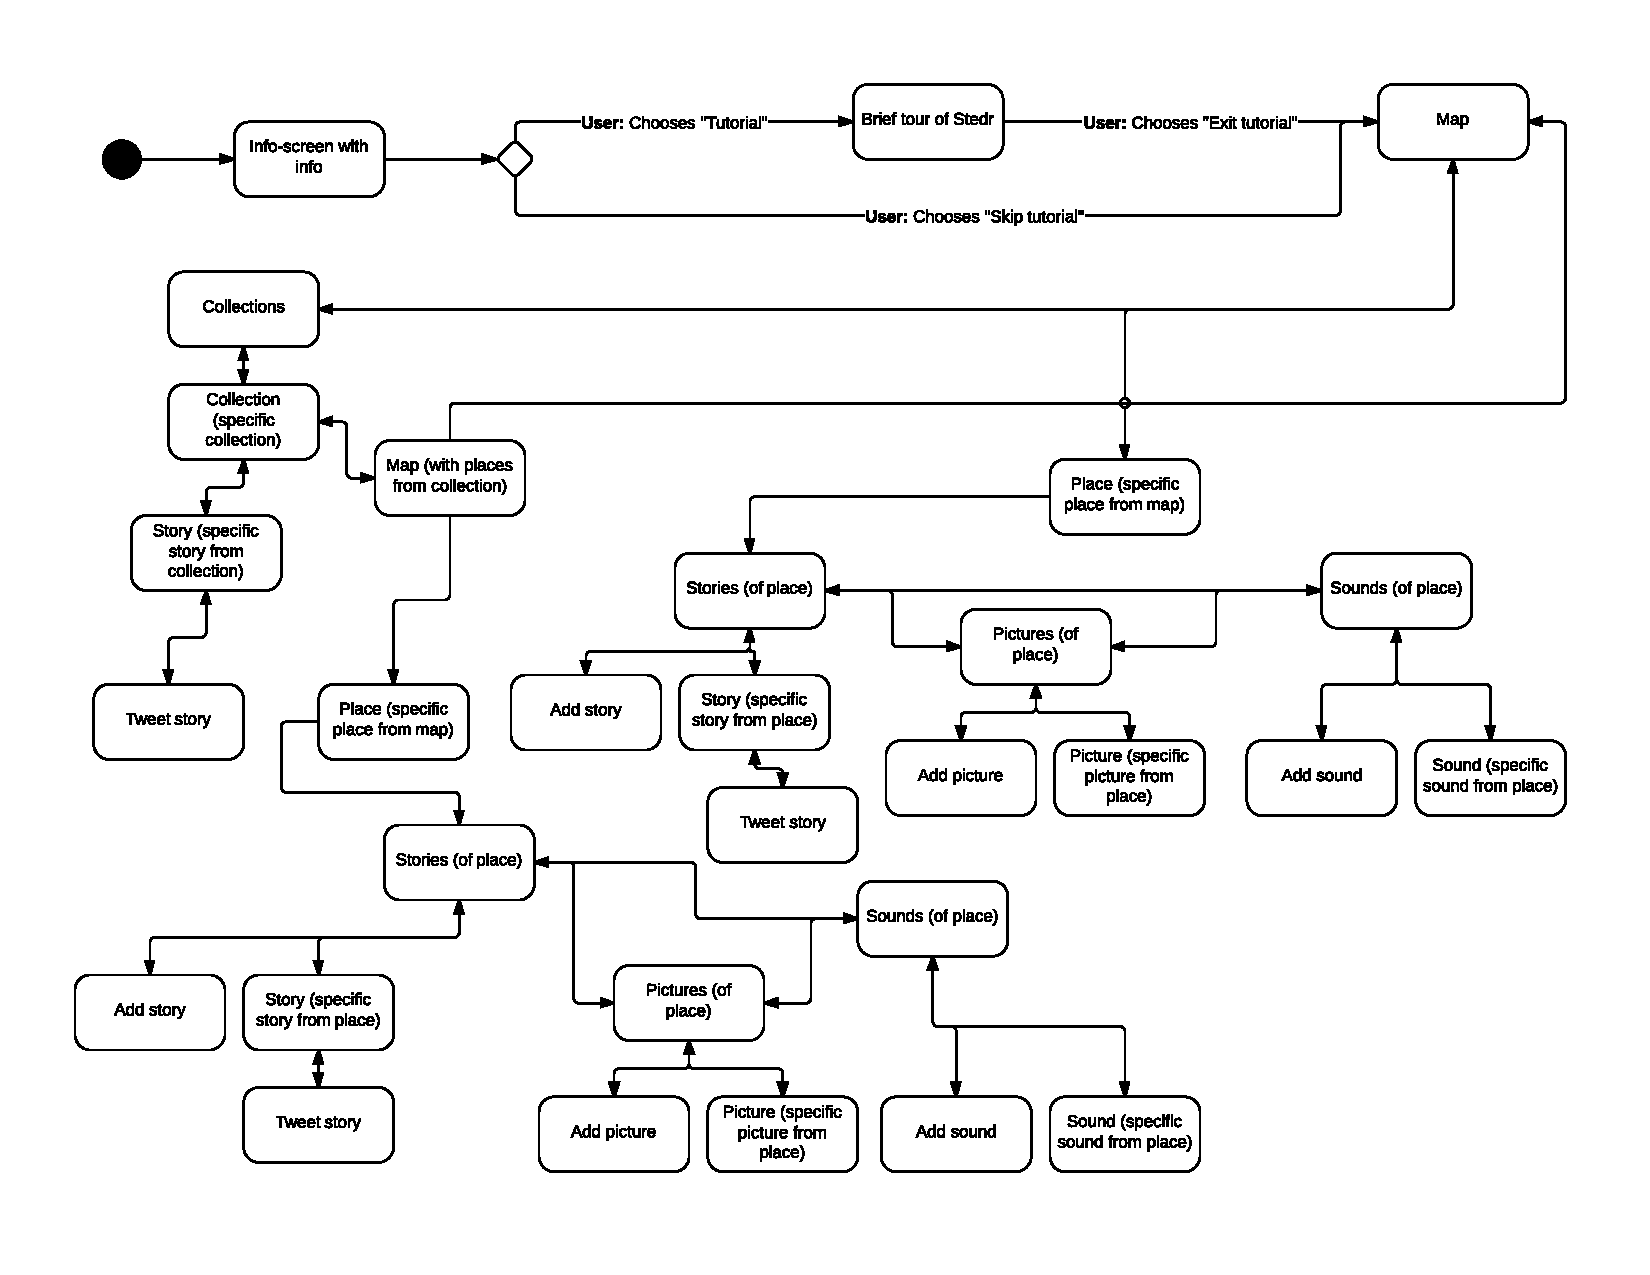
\includegraphics[width=1\textwidth]{res/processView.pdf}
\caption{Process View}
\end{center}
\end{figure}


\subsection{Use Case}

\begin{figure}[!h]
\begin{center}
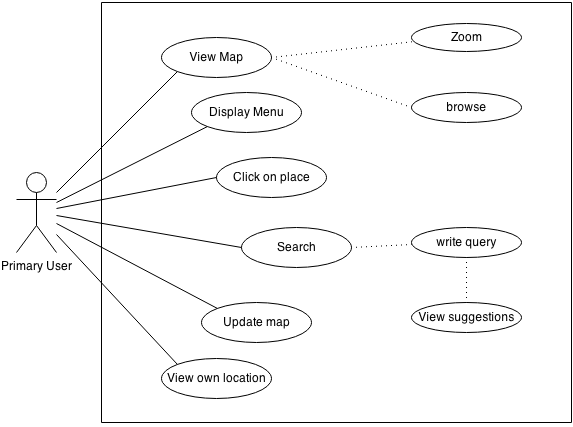
\includegraphics[scale=0.6]{ms.png}
\caption{Map View (Home)}
\end{center}
\end{figure}

\begin{figure}[!h]
\begin{center}
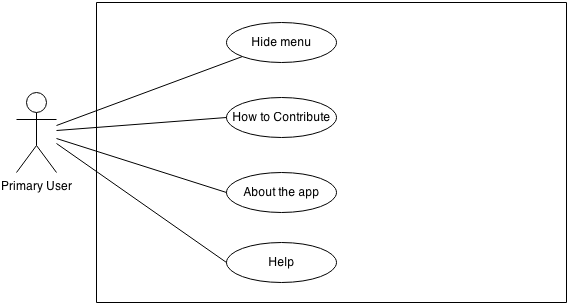
\includegraphics[scale=0.6]{mens.png}
\caption{Menu View}
\end{center}
\end{figure}

\begin{figure}[!h]
\begin{center}
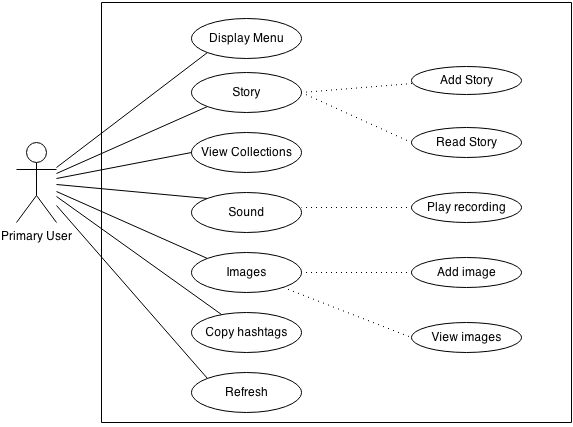
\includegraphics[scale=0.6]{ps2.png}
\caption{Place Screen}
\end{center}
\end{figure}

\clearpage

\subsection{Sequence}

\begin{figure}[!h]
\begin{center}
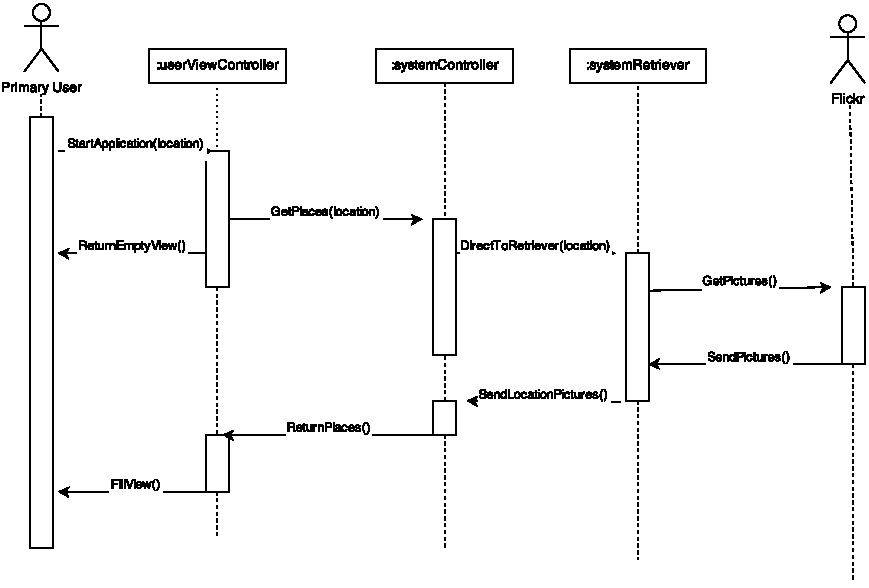
\includegraphics[scale=1]{Get-Stories}
\caption{Get Stories}
\end{center}
\end{figure}

\begin{figure}[!h]
\begin{center}
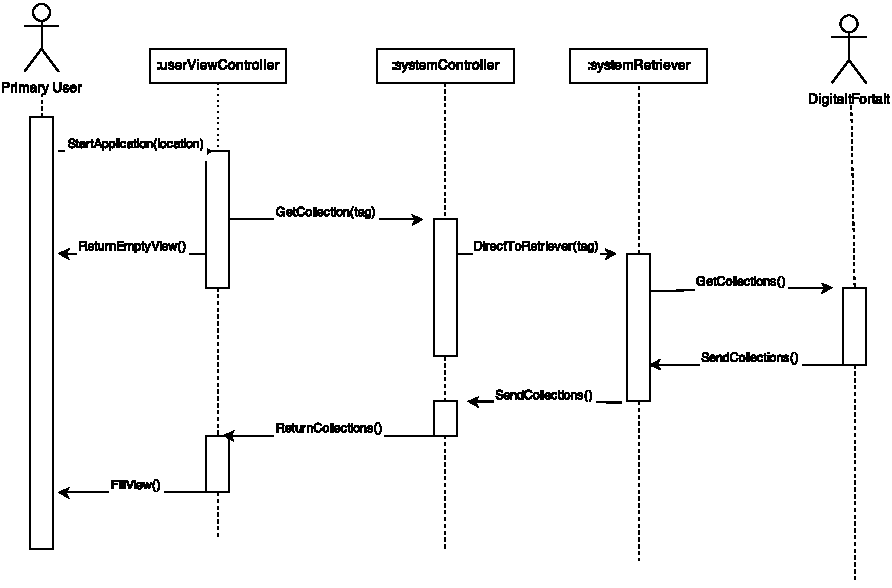
\includegraphics[scale=1]{Get-Collections}
\caption{Get Collections}
\end{center}
\end{figure}
\clearpage 					%This command flushes out all the queued floats waiting to be placed to avoid them being placed inapropriately in another section.
\section{Implementation}


\subsection{Sprint 1}
\subsection{Sprint 2}
\subsection{Sprint 3}
\subsection{Sprint 4}
\subsection{Sprint 5}
\subsection{Sprint 6}
\clearpage

\section{Testing}
\thispagestyle{plain}
System testing or software testing, falls into something that is called “Black-box testing”. This is a method of software testing, that investigates the functionality of the application, eg. what it does. It will not interfere with it's internal structure or workings. 

\subsection{Testing Procedure}

When you are about to conduct a test, you find a test-person. Then you tell them what the software is supposed to do and further give them the Test cases[7.2]. It is very important for the test subjects to think loud so we can get maximum feedback from the testing. 

\subsection{Test Cases}

Test cases are built around the specifications and requirements of the application. What the application is supposed to do.  

\begin{table}[htp]
\begin{center}
\begin{tabular}{ i{4cm} ||  i{10cm}} \toprule
\multicolumn{2}{c}{\textbf{Get Places}} \\ \hline
ID & T-F1 \\ \hline
Requirements & SF-1 \\ \hline
Feature& Places are shown on the map \\ \hline
Preconditions& \begin{enumerate} \item Flickr is up \item The Flickr group contains photos with locations \item Application is installed on device \item Device is connected to the internet \end{enumerate} \\ \hline
Test Description& \begin{enumerate} \item Open the application \item Wait for 30 seconds \item Click on a pinpoint \item Zoom out to a world view  \end{enumerate} \\ \hline
Expected result & The map should show some clickable pinpoints. When clicked the pinpoints should open a little box containing a thumbnail picture and small text provided by the Flickr Stedr group. \newline
When zoomed out new places should be loaded according to what the user see. \\ \hline
Pass/Fail criteria & The test is considered a pass if the expected result happens. The last step that need to be passed is that the place at Grenada is shown. \newline
If there are any inconsistencies with the expected result, the test should be considered a fail. \\ \hline
Severity & High\\ \bottomrule
\end{tabular}
\end{center}
\caption{Test Case: Get Places}
\label{tab:Test Case: Get Places}
\end{table}


\begin{table}[htp]
\begin{center}
\begin{tabular}{ i{4cm} ||  i{10cm}} \toprule
\multicolumn{2}{c}{\textbf{Open menu}} \\ \hline
ID & T-F2 \\ \hline
Requirements & SF-2 \\ \hline
Feature& Drawer menu with options is opened. \\ \hline
Preconditions& \begin{enumerate} \item[ ]1,2,3,4 \end{enumerate} \\ \hline
Test Description& \begin{enumerate} \item Click on the menu button \item Click on all of the icons in the menu \item Click on the menu again \end{enumerate} \\ \hline
Expected result & When the menu button is pressed, a drawer menu should open. All of the icons in the drawer menu is also buttons and when clicked again, the menu button should close the drawer menu. \\ \hline
Pass/Fail criteria & The test is considered a pass if the menu button opens and closes a drawer menu. Also, all of the icons should \\ \hline
Severity & High\\ \bottomrule
\end{tabular}
\end{center}
\caption{Test Case: Open Menu}
\label{tab:Test Case: Open Menu}
\end{table}


\begin{table}[htp]
\begin{center}
\begin{tabular}{ i{4cm} ||  i{10cm}} \toprule
\multicolumn{2}{c}{\textbf{Views}} \\ \hline
ID & T-F3 \\ \hline
Requirements & SF-6 \\ \hline
Feature& All the views are accessible \\ \hline
Preconditions& \begin{enumerate} \item[ ]1,2,3,4 \item[T-F1] Get places \end{enumerate} \\ \hline
Test Description& \begin{enumerate} \item Click on a pinpoint \item Click on the small window that appears \item Click on one of the buttons \textit{Images, Sound, Story} \item Dependent on the previous step, click on the buttons not yet pushed \item Click the menu button \item Click home \end{enumerate} \\ \hline
Expected result & Which view that is selected is shown to the user by being in a different colour than the two other buttons. If the button for the selected view is touched, nothing should happen. \newline
For every button representing a non-selected view, the user should be taken to the view as indicated by the button text. \\ \hline
Pass/Fail criteria &The test is passed if the button: \newline[5pt]
Image - Takes you to the image view\newline
Story - Takes you to the story view\newline
Sound - Takes you to the sound view.\newline[5pt]
The selected view has a unclickable button in a different colour representing the selected view.\newline
Considered a fail if there are any inconsistencies with the criteria above. \\ \hline
Severity & High\\ \bottomrule
\end{tabular}
\end{center}
\caption{Test Case:  Views}
\label{tab:Test Case: Views}
\end{table}


\begin{table}[htp]
\begin{center}
\begin{tabular}{ i{4cm} ||  i{10cm}} \toprule
\multicolumn{2}{c}{\textbf{Load Content}} \\ \hline
ID & T-F4 \\ \hline
Requirements & SF-7 \\ \hline
Feature& Content is loaded for the places \\ \hline
Preconditions& \begin{enumerate} \item[T-F3] Views \end{enumerate} \\ \hline
Test Description& \begin{enumerate} \item Click on a pinpoint(not Camera Obscura) \item Click on the description \item Go through the views as in T-F3 \item[3a] Click on all of the titles on the story \item[3b] Click on two random images \item[3c] Click on a sound \end{enumerate} \\ \hline
Expected result & The places should be loaded with relevant and accessible content from all of the content providers.. \newline
If some content-types are not provided for the specific place, the content type should be loaded but indicate that it is empty. \\ \hline
Pass/Fail criteria &The test is considered a pass if the expected result happens. \newline
If there are any inconsistencies with the expected result, the test should be considered a fail. \\ \hline
Severity & High\\ \bottomrule
\end{tabular}
\end{center}
\caption{Test Case: Load Content}
\label{tab:Test Case: Load Content}
\end{table}



\begin{table}[htp]
\begin{center}
\begin{tabular}{ i{4cm} ||  i{10cm}} \toprule
\multicolumn{2}{c}{\textbf{Collection view}} \\ \hline
ID & T-F5 \\ \hline
Requirements & SF-8 \\ \hline
Feature& Show a view with the stories related to a collection \\ \hline
Preconditions& \begin{enumerate} \item[T-F2] Open menu \item[T-F4] Load Content \item[5] It exist a collection \end{enumerate} \\ \hline
Test Description& \begin{enumerate} \item Press the menu button \item Press the Collection button \item Press a collection \end{enumerate} \\ \hline
Expected result & When the collection button is pressed a new view should open with the list of stories related to the collection. \\ \hline
Pass/Fail criteria & The test is considered a pass if it is possible to open the menu and access a collection with a list of stories. \\ \hline
Severity & Medium\\ \bottomrule
\end{tabular}
\end{center}
\caption{Test Case: Collection View}
\label{tab:Test Case: Collection View}
\end{table}


\begin{table}[htp]
\begin{center}
\begin{tabular}{ i{4cm} ||  i{10cm}} \toprule
\multicolumn{2}{c}{\textbf{Collection map view}} \\ \hline
ID & T-F6 \\ \hline
Requirements & SF-8 \\ \hline
Feature& Show places related to a collection as pinpoints in a map \\ \hline
Preconditions& \begin{enumerate} \item[T-F2] Collection View \end{enumerate} \\ \hline
Test Description& \begin{enumerate} \item Press the menu button \item Press the Collection button \item Press a collection \item Press the \textit{show on map}-button \end{enumerate} \\ \hline
Expected result &When the “show on map”-button is clicked, a map view should open with related places showed as pinpoints. Pinpoints not related to the collection should not be placed on the map. \\ \hline
Pass/Fail criteria & The test is considered a pass if all places related to a collection is exclusively shown in a map view. \\ \hline
Severity & Medium\\ \bottomrule
\end{tabular}
\end{center}
\caption{Test Case: Collect Map View}
\label{tab:Test Case: Collect Map View}
\end{table}


\begin{table}[htp]
\begin{center}
\begin{tabular}{ i{4cm} ||  i{10cm}} \toprule
\multicolumn{2}{c}{\textbf{Gallery}} \\ \hline
ID & T-F7 \\ \hline
Requirements &  \\ \hline
Feature& Gallery function\\ \hline
Preconditions& \begin{enumerate} \item[T-F4] Load Content \item[ ] The application is in a place with a story where there are multiple images to the story. \end{enumerate} \\ \hline
Test Description& \begin{enumerate} \item Press the story title \item If there are more pictures related to a story, press the arrows \end{enumerate} \\ \hline
Expected result &When accessing stories with multiple pictures as content, arrows indicating the possibility to go through picture files should appear. When pressed new images should replace the old picture. \\ \hline
Pass/Fail criteria &The test is considered a pass if the expected result happens. \newline
If there are any inconsistencies with the expected result, the test should be considered a fail. \\ \hline
Severity & Low\\ \bottomrule
\end{tabular}
\end{center}
\caption{Test Case: Gallery}
\label{tab:Test Case: Gallery}
\end{table}


\begin{table}[htp]
\begin{center}
\begin{tabular}{ i{4cm} ||  i{10cm}} \toprule
\multicolumn{2}{c}{\textbf{Upload Content}} \\ \hline
ID & T-F8 \\ \hline
Requirements &  SF-9\\ \hline
Feature& Content can be uploaded to Instagram, Twitter and SoundCloud \\ \hline
Preconditions& \begin{enumerate} \item[T-F4] Load Content \item[6] Successfully connected to the content (not story provider) providers \end{enumerate} \\ \hline
Test Description& \begin{enumerate} \item Click on a pinpoint \item Click on the description \item Go through the views as in T-F3 \item Upload textual content to Twitter \item Upload picture to Instagram \item Upload sound to SoundCloud \end{enumerate} \\ \hline
Expected result &The places should be loaded with relevant and accessible content from all of the content providers..\newline
If some content-types are not provided for the specific place, the content type should be loaded but indicate that it is empty. \\ \hline
Pass/Fail criteria & The test is considered a pass if the expected result happens. \newline
If there are any inconsistencies with the expected result, the test should be considered a fail. \\ \hline
Severity & Medium\\ \bottomrule
\end{tabular}
\end{center}
\caption{Test Case: Upload Content}
\label{tab:Test Case: Upload Content}
\end{table}

\clearpage

\subsection{Test Execution}
\label{sec:TestExecution}
\subsubsection{System Testing}

During the final stages of the development, it was performed a system test after integrating all of the developed components. This was an important step done before the acceptance testing, to see that all of the components developed by different team members and the former development team worked together. Since we did not have the resources it was impossible to let an external team do the testing, but to emulate some sort of indipendence to the system the tests were done by a group member who had been less involved in the development of the client and never tried the client on a smartphone. This of course is a weakness in the testing, since the tester had a general knowledge of the system worked and also a basic idea of the client from using the system on a smartphone emulator.

A summary of the test results is shown in the table below, and an example from the test log can be found in the appendix \ref{sec:TestLog}

\begin{table}[!htp]
\begin{center}
	\begin{tabular}{ | l | l | l | }
	\hline
	\textbf{ ID} 	& \textbf{Verdict}		& \textbf{Comment} 	\\ \hline
	T-F1		&Unknown		& Valid with full cache, not valid when empty cache	\\ \hline
	T-F2		&Pass		& None	\\ \hline
	T-F3		&Pass		& None	\\ \hline
	T-F4		&Pass		& None	\\ \hline
	T-F5		&Pass		& None 	\\ \hline
	T-F6		&Pass		& None 	\\ \hline
	T-F7		&Pass		& None 	\\ \hline
	T-F8		&Fail			& This feature was declared infeasible  	\\ 
	 \hline
 	 \end{tabular}
\end{center}
\caption{System Testing: Validity}
\label{tab:System Testing: Validity}
\end{table}

\subsubsection{Acceptance Testing}

Acceptance testing is one of the last levels of the software testing process. The purpose of such testing is to evaluate the system's compliance with the given requirements to check whether it is acceptable for delivery. Hence the name acceptance testing.

On May 14. during one of our last meetings we sat down with Jacqueline Floch for the final acceptance test of our system. This acceptance test included further developed features and improvements of the graphical user interface.

For the main test we had a feature based acceptance test where we went through the requirement list. Not to say that usability is not as important, but our customer had received the latest build almost every week in the later stages of the project. With this, the customer have conducted usability acceptance testing regularly throughout the project, giving us feedback. Because of this we did not have the same need for a usability based user acceptance test, which we know is the norm, but Jacqueline Floch had the app tested by four of her colleagues, which all gave positive feedback. If there had been any crucial shortcomings it probably would have been pointed out.

The test was conducted by going through the requirement list sorted by priority and individually receiving a verdict on acceptance. The individual requirement either reviewed \texttt{Pass, fail, outdated} or \texttt{cancel} if the requirement was withdrawn. The latter was the case on a lot of the requirements with lower priority since we had little time and the customer wanted us to focus on the more important tasks.

The result of the acceptance test are listed below:\\

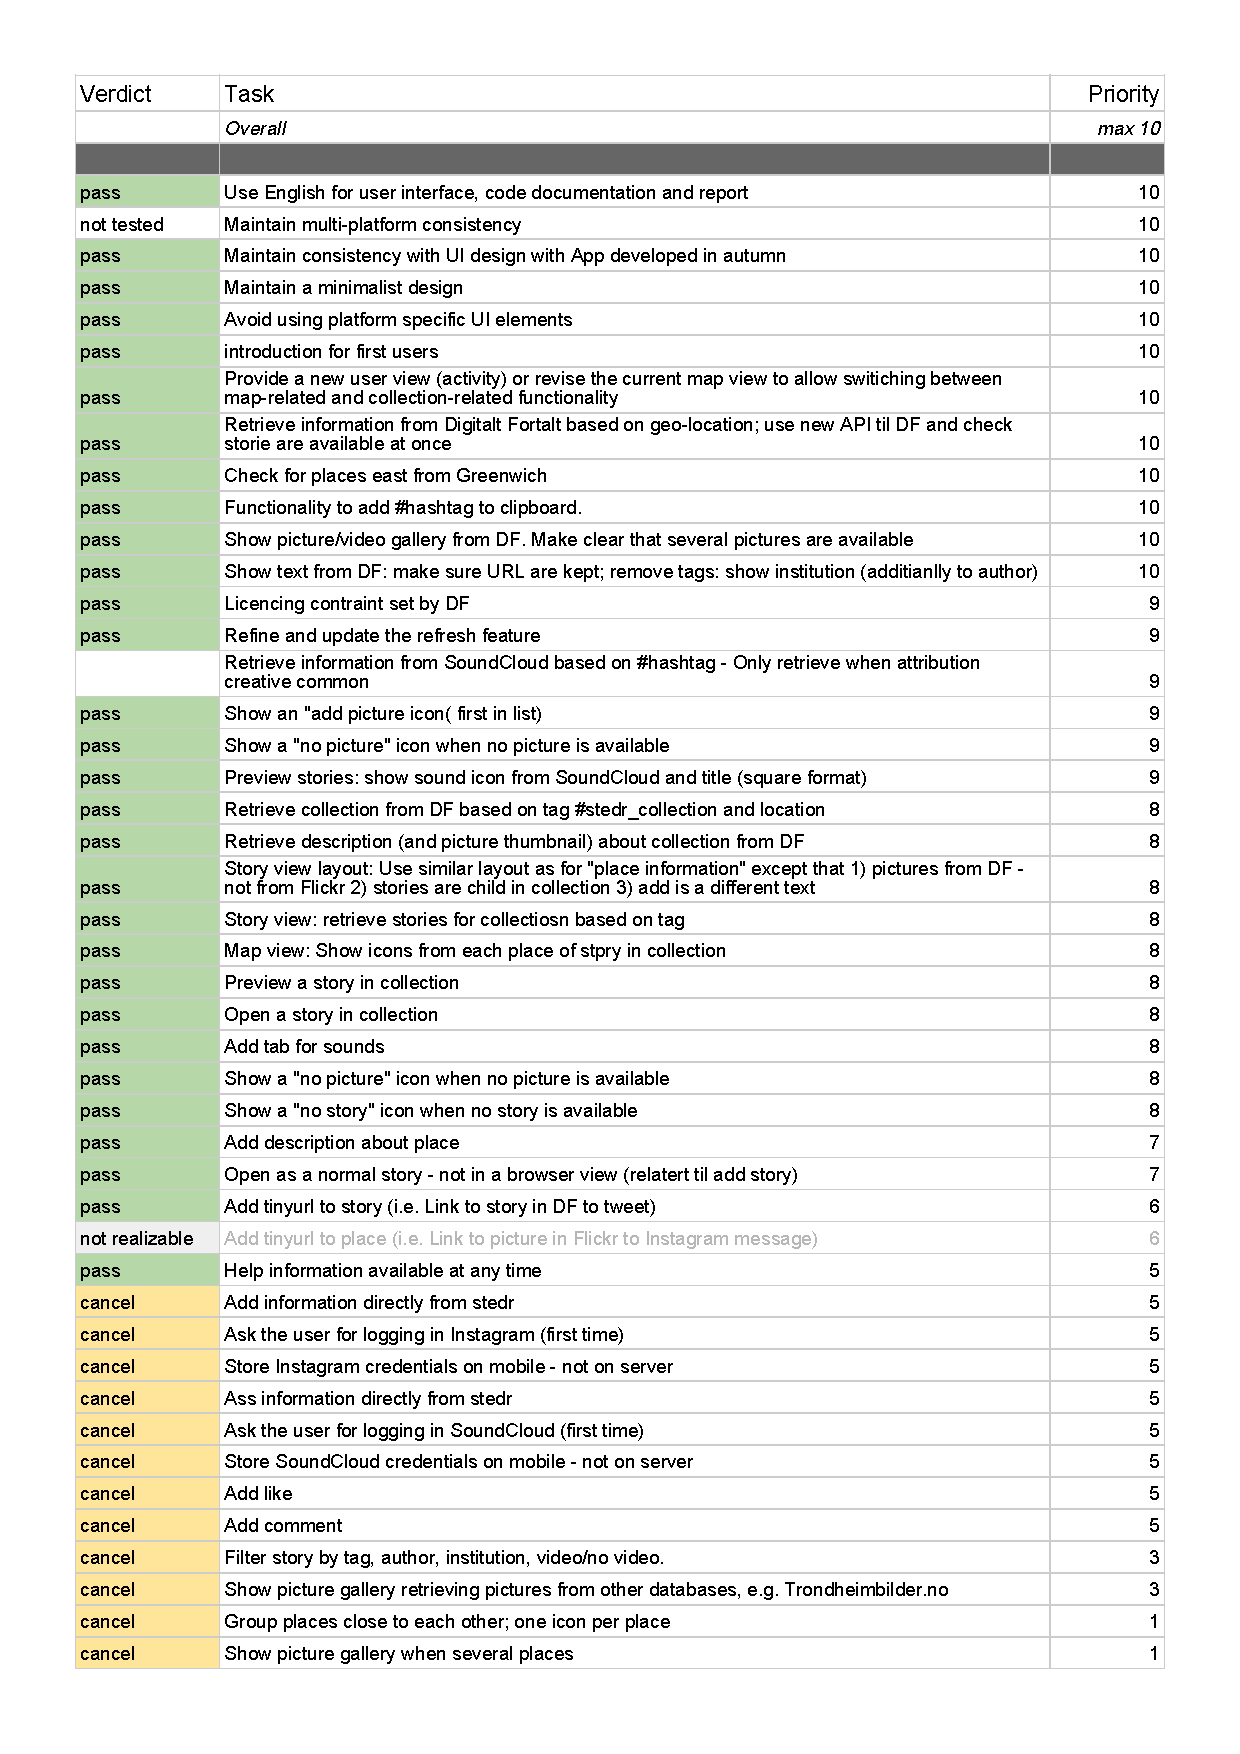
\includepdf[%
 	pages={-},
	offset=0in 0in,%
	]{res/AcceptanceTesting_Requirements.pdf}
\label{sec:featList}
As you can see, one requirement are missing a verdict. This is is because this was not testable since we waited for a response from SoundCloud at the time. This was later implemented and are now working as it should.


\subsubsection{NFR testing}
It is important for the project that our result meets the projects main non-functional requirements, described in the ``Product quality'' section of the SRS chapter (\ref{sec:ProductQuality}), for it to be considered a success. 

\paragraph{Compability}

\emph{Co-existence}
With the result found under Reliability - maturity, it is clear that the system can handle that multiple client share the same environment. It is worth to notice that the testing program makes use of threads to be more realistic regarding parallel requests to the server.

\emph{Interoperability}
Since the requirement for interoperability was said to be fulfilled as long as the system followed a standardized method of communication over a known and widely used protocol, the testing consisted of looking at the objects sent from the server and acknowledge that they were valid JSON-objects.

\begin{table}[!htp]
\begin{center}
	\begin{tabular}{ | l | l | l | }
	\hline
	 \#	 	& Content 		& JSON 	\\ \hline
	 1		&Places		& Yes	\\ \hline
	 2		&Stories		& Yes	\\ \hline
	 3		&Images		& Yes	\\ \hline
	 4		&Collections	& Yes	\\ \hline
	 5		&Sound		& Yes 	\\
	 \hline
 	 \end{tabular}
\end{center}
\caption{Compability: Interoperability}
\label{tab:Compability: Interoperability}
\end{table}

\paragraph{Performance Efficiency}
We have greatly improved the core of the system to boost the efficiency of the application. This should cause the application to use no more than 300 seconds to pull new content from the APIs. The efficiency was tested by adding new content and recording 10 times with different content posted at different times. By measuring the individual response times and calculating the average result we will get a rough estimate.\\

\begin{table}[!htp]
\begin{center}
	\begin{tabular}{ | l | l | l | r | }
	\hline
	 \#	 	& Content 		& Time a day 		& Result \\ \hline
	 1		&Instagram		& 10:55			& \texttt{1 sec} \\ \hline
	 2		&Instagram		& 14:40			& \texttt{1 sec} \\ \hline
	 3		&Instagram		& 14:45			& \texttt{1 sec} \\ \hline
	 4		&Tweet		& 14:16			& \texttt{19 sec} \\ \hline
	 5		&Tweet		& 14:18			& \texttt{20 sec} \\ \hline
	 6		&Tweet		& 10:40			& \texttt{20 sec} \\ \hline
	 7		&Story		& 15:26			& \texttt{133 sec}\\ \hline
	 8		&Story		& 16:15			& \texttt{10 sec}\\ \hline
	 9		&Story 		& 11:00			& \texttt{104 sec}\\ \hline
	 10		&Story		& 15:48			& \texttt{135 sec}\\ \hline
	 11		&Story		& 16:03			& \texttt{107 sec}\\ \hline
	 13		&Story		& 19:01			& \texttt{132 sec}\\ \hline
	 14		&SoundCloud		& 18:51			& \texttt{5 sec}\\ \hline
	 15		&SoundCloud		& 19:15			& \texttt{7 sec}\\ \hline
	 16		&SoundCloud		& 19:20			& \texttt{6 sec}\\  
	 \hline
 	 \end{tabular}
\end{center}
\caption{Performance Efficiency: Publishing New Content}
\label{tab:Performance Efficiency: Publishing New Content}
\end{table}

Since much of the test content had relatively consistent results we did not think more testing was needed. The Instagram images appeared almost instantly ( 1 second) consistently, since we completed the tests manually, we could not measure finer times. The twitter content were a little slower as expected, but did also appear consistently at a reasonable time averaging in just under 20 seconds. The SoundCloud publishing also happened pretty quick averaging \texttt{6 seconds} As for the stories we published through Digitalt Fortalt, the times were very inconsistent. In three of the tests (\# 7, \#10 and \#12), which was the longest ones, the content had to be uploaded to DF as well as being published. This probably added to the time. All the other tests were performed with the content already uploaded, but we still recorded a massive variation in results ranging from \texttt{10 seconds} (\#8) to \texttt{105 seconds} (\#9).


Average: 
\begin{equation}
\frac{133 + 10 + 104 + 135 + 107 + 132}{6} = {103.5}
\end{equation}

With all results clocking in under 150 seconds, and our goal being under 300 seconds, we are very pleased with the results and can happily see our app passing this test. Considering that the original app needed multiple days for the results to appear, it is needless to say that there have been a massive improvement.


Another important part of the performance efficiency is the application's data usage. Blowing the users' data limit and potentially taking a large part in increasing their phone-bill is something we want to avoid. To avoid this we have implemented a data usage restraint. This restraint is set through equation (\ref{eq:DownloadLimit}) in section \ref{sec:ProductQuality}.

We tested the data usage to make sure our application met our standard. We measured this roaming unconnected to any WiFi-hotspots while running the app.\\

\emph{Quick session}\\
Opening map: \texttt{55.74 kB}\\
Entering place with only one story: \texttt{+ 6.07 kB}

\emph{Browsing session}\\
Browsing map over Trondheim: \texttt{1.64 MB}\\
Entering place with 6 stories and 2 Instagram pictures: \texttt{+ 0.02 MB}

We found these results to be pretty reasonable. The app does not download more content than necessary, and the results seems really consistent compared to the experiences we have had using the application.

\paragraph{Reliability}

Testing of components was done by feeding test cases to the components. When accepted, these new components was added to a running server instance that acted as a beta. The beta server was deployed at the 9th of April and has since been monitored to record uptime and errors. Shortly after Easter the old server was changed with the new one so that the customer could use new features, but also so that it was possible to monitor how the server performed under normal usage.

A shortcoming to the test-data below is that each time new features was deployed to the server, the server was restarted. Because of this, the longest interval the server has been running uninterrupted is approximately one week. 

\emph{Maturity}\\
The testing of maturity was done by analysing the data recorded in comparison to the feedback we got from the customer. Also, there was done an additional test where specific task were completed. Since maturity considers the system under normal use, the additional test was not a stress test in terms of using the system until it broke. Rather it was using the system at a relatively high frequency and noting the number of incidents.

To simulate users we made a testing program which made a total of 500 requests over a short period of time ($<5 minutes$). This test was done eight times over a single day, but with random rest periods for the server. If the server returned an error this was noted. 

\begin{table}[!htp]
\begin{center}
	\begin{tabular}{ | l | l | l | p{7cm} | }
	\hline
	\#	&Time since last test &Number of errors	& Notes \\ \hline
	1	&NA			& 1 & Places do not load. This also disables all other content retrievers\\ \hline
	2	&30 minutes		& 0 & Stories do not load. Does not affect other parts of the system\\ \hline
	3	&60 minutes		& 1 & Instagram pictures do not load. Does not affect other parts of the system\\ \hline
	4	&10 minutes		& 0 & Sounds do not load. Does not affect other parts of the system\\ \hline
	5	&120 minutes	& 1 & Total systems fail\\ \hline
	6	&60 minutes		& 1 & Places do not load. This also disables all other content retrievers\\ \hline
	7	&10 minutes		& 0 & Stories do not load. Does not affect other parts of the system\\ \hline
	8	&60 minutes		& 1 & Instagram pictures do not load. Does not affect other parts of the system\\
	 \hline
	 \end{tabular}
\end{center}
\caption{Maturity Testing}
\label{tab:Maturity Testing}
\end{table}

The test results clearly shows that there is a problem when the server has been inactive for more than an hour. This is because the server keeps a cache of places for an hour, before it deletes the cache. After the cache is emptied the server waits for a request before it again repopulates the cache. Also, when the server requests Flickr for new places it throws a time-out error. The time-out error doesn't have an effect for the user other than that the application is a bit slow if the user is the first to use the system after the cache has been emptied.

\emph{Availability}\\
Since the customer started using the new server (23rd of April) the server has been functional continuous, except from the 6th to the 7th of May. This gives that the system has had an uptime under presumably normal use of:

$1-\frac{24 hrs}{23 days \times 24 hours} \times 100 = 95.652 \% $

\emph{Fault tolerance}\\
The systems fail noted under the availability test was due to an global error on one of the systems external system. From this it is clear that the system depends totally on some of it's components and thereby external systems to provide the required functions. To determine how many critical components that exists in the systems, every component in the system was disabled to see the effect on the system. In addition, another part of the test considered interrupting connections to external systems. 

Note that to be considered functional, the system had to show places and load stories to the end-user. 

\begin{table}[!htp]
\begin{center}
	\begin{tabular}{ | l | p{4.2cm} | l | p{6.5cm} | }
	\hline
	\#	&Disabled Component	&Functional system	& Notes \\ \hline
	1	&Flickr Retriever		&No			& Places do not load. This also disables all other content retrievers\\ \hline
	2	&Story Retriever		&No			& Stories do not load. Does not affect other parts of the system\\ \hline
	3	&Picture Retriever	&Yes			& Instagram pictures do not load. Does not affect other parts of the system\\ \hline
	4	&Sound Retriever	&Yes			& Sounds do not load. Does not affect other parts of the system\\ \hline
	5	&External component (Heroku)	&No			& Total systems fail\\ \hline
	6	&External component (Flickr)	&No			& Places do not load. This also disables all other content retrievers\\ \hline
	7	&External component (Digitalt Museum)	&No		& Stories do not load. Does not affect other parts of the system\\ \hline
	8	&External component (Instagram)	&Yes			& Instagram pictures do not load. Does not affect other parts of the system\\ \hline
	9	&External component (Soundcloud)	&Yes			& Sounds do not load. Does not affect other parts of the system\\ 
	 \hline
	 \end{tabular}
\end{center}
\caption{Fault Tolerance Testing}
\label{tab:Fault Tolerance Testing}
\end{table}

This describes a major drawback of the reliability of the system, out of the four retrievers there are two single points of failure. In addition, the system also depends on three of five external systems to function properly. It is also important to note that if any of the external systems make radical changes so the system components becomes outdated, this will also lead to a non-functional system. Because of this the system cannot say to satisfy the requirement for fault tolerance.

\emph{Recoverability}\\

Testing for recoverability was done together with the testing for fault tolerance, by taking the time on how long it took for the system to be functional after re-enabling an external or internal components. Since the system isn't a critical system, the timing requirement was set to five minutes, so to pass the recoverability requirement the system should function normally within five minutes of the component re-enabling. 

\begin{table}[!htp]
\begin{center}
	\begin{tabular}{ | l | l | p{3.7cm} | r | }
	\hline
	\#	&Disabled Component	&Functional system  after five minutes	& Notes \\ \hline
	1	&Flickr Retriever		&Yes			& $<5 minutes$ \\ \hline
	2	&Story Retriever		&Yes			& $<5 minutes$\\ \hline
	3	&Picture Retriever	&Yes			& $<5 minutes$\\ \hline
	4	&Sound Retriever	&Yes			& $<5 minutes$\\ \hline
	5	&External component (Heroku)	&Yes			& $<5 minutes$\\ \hline
	6	&External component (Flickr)	&No			& $<60 minutes$\\ \hline
	7	&External component (Digitalt Museum)	&Yes		& $<5 minutes$\\ \hline
	8	&External component (Instagram)	&Yes			& $<5 minutes$\\ \hline
	9	&External component (SoundCloud)	&Yes			& $<5 minutes$\\ \hline
	 \hline
	 \end{tabular}
\end{center}
\caption{Recoverability Testing}
\label{tab:Recoverability Testing}
\end{table}

Because of a cache used to store places provided by Flickr, the system uses up to 60 minutes to refresh the cache. This means that errors so that Flickr doesn't respond to requests, leaves the system with an empty cache and thereby no places. This will again lead to a failure of the FlickrRetriver and the system itself as describes under the Fault Tolerance Test. 

\paragraph{Portability}

The multiplatform aspect of the project has played a major part in the choice of environment and frameworks. What we want to achieve is a reasonable consistency through different platforms and versions. We have throughout the development process tested it with many different virtual devices on different settings, but the most valuable ones are the ones performed on the physical devices at our disposal. As previously mentioned, we have unfortunately not had it tested on any iOS devices.\\

\begin{table}[!htp]
\begin{center}
	\begin{tabular}{ | l | l | l | r | }
	\hline
	 \#	& Platform (version)			&Device					& Notes \\ \hline
	 1	&Android (4.4.2 KitKat)			&LG Nexus 5 (3 different devices)	& Works fine\\ \hline
	 2	&Android (4.1 Jelly Bean)			&Samsung Galaxy SII			& Works fine\\ \hline
	 3	&Android (4.3 Jelly Bean)			&Samsung Galaxy Nexus			& Works fine\\ \hline
	 4	&Android (4.2 Jelly Bean)			&HTC One					& Works fine\\ \hline
	 5	&Android (4.0 Ice Cream Sandwich)	&Huawei Mediapad tablet			& Works fine\\ \hline
	 6	&Android (4.3 Jelly Bean)			&Sony Xperia Z1				& Works fine\\
	 \hline
	 \end{tabular}
\end{center}
\caption{Portability Testing}
\label{tab:Portability Testing}
\end{table}

\clearpage
\section{Evaluation}
\thispagestyle{plain}
	\subsection{Process}

With our process modell, Scrum, we found that following it by the book, became very troublesome. Therfore we decided to make some modification to the original model. The main problem with using Scrum by the letter is that we are all students, and this project only counts for half of the semesters study points. This means we all have different schedules, and thus making it difficult to have daily meetings. End meetings, or retrospective meetings is also something we haven’t prioritized much.

In Scrum it is common to use something called planning poker when deciding how long tasks should take. This essentially means that everyone “votes” on how time consuming they think a given task will be. We found this to be a little unnecessary because its usually so imprecise, and have therefore chosen to just let the persons responsible give their judgements to save time. 

	\subsection{Project Management}

One of the main challenges for us concerning project management was the frequent changes made in regards to features. It also took a while to come to a shared view on the requirements with our customer. Later in the project, the customer provided us with a long list with about 50 features that was to be implemented. We ended up treating requirements different from this feature list. This was because, even though our requirements addressed much of the features in the feature list, they were still on a another abstract level. The feature list items was too detailed and specific to be listed as requirements.

	\subsection{Communication}

We feel that the communication internally on the team have been good. By using different channels like Facebook, mail, and phone, we were able to stay in touch throughout the project even though we couldn't always be physically present on the school.

With the customer on the other hand, the communication could have been handled better on both parts. 

Our customer went on an unfortunate sick leave at the start of the project, which ment that our communication had to go through a third party. At first, it didn't seem like a big problem, but when we later discovered how this had led to major misunderstandings, it ended up hurting us more than we first thought it would.

About three weeks into the project, we started to have direct communication with our customer over skype once a week. These meetings didn't work well for us. It made it hard for everybody to engage in the conversations. Altough we always paid attention and were careful to write summaries from these meetings, the customer's visions didn't get trough to us somehow. We thought we had a clear picture of what our customer wanted, but it turned out to be wrong.

It wasn't really untill we started meeting our customer in person, halfway in to the project, that we understood how much we had been talking past each other. There had been lacking clarity in messages between us and since both parts thought they understood each other, no measures where made. Now, after an almost four hour meeting with our customer in person, we finally came to an common understanding of what purpose the app had. This also meant that we suddenly was far behind schedule since we had to completely redo the product backlog based on the new feature list. We strongly feel that this list should have been provided to us at the beginning of the project. It would have saved us a lot of time.

That being said, we also take self criticism. There was for instance one incident where a team members didn't pay enough attention on a meeting. This resulted in him working almost 20 hours with trying to integrate the soundcloud UI experience into StedR. What our customer really wanted was for us to make a simple api call to the Soundcloud servers and retrieve sounds based on title. We of course take full responsibility for this. 


	\subsection{Project planning}


Our pre-study and project planning was really thorough, but in retrospective, much of it ended up being a waste. We spent a lot of time doing research and user tests, trying to figure out what direction we should take the app in. Because of the misunderstanding explained in Communication, we thought we had much more freedom than we actually had. We had the idea that we could just get creative and play with the app as we saw fit.

Its not that we have any problems of working with a predefined feature list, but then it should be clear that we in fact have these restraints.

In the first half of the project, these were some of the features we were working on that we later dismissed:

\begin{itemize}
	\item Adding new places from the app
	\item Wikipedia integration - Possebility to see wiki entires related to the place you are visiting.
	\item Adding full Soundcloud experience in the app.
	\item Attaching NRK archive footage to a place. 
	\item General design overhaul.  (Dismissed mockups can be found in \todo{appendix X})
\end{itemize}

	\subsection{Problems and difficulty}

The development of this app have been quite a bumpy ride for us. We have stumbled upon surprisingly many problems from our risk analysis.

One could of course question our preventive abilities, but we still feel we took the right precautions. Some things are just left to luck.

From out risk analysis, this is some of the more important problems we came across in this project. 

\begin{itemize}
	\item Communication failure - Between the team and the customer as explained in Communication.
	\item Major requirements change - The new feature list, which was given to us halfway into the project, changed the requirements a lot.
	\item Technical difficulties - We had huge trouble setting up the development environment for titanium framework. Two team members didn't even get it to work at all.
	\item Unavailability - Two team members spent 2 weeks in china which reduces our capacity right before easter. 
	\item Lack of Competence - Combined we had zero experience with some of the technologies used in this project beforehand.
	\item Sickness - As explained above.
	\item Equipment Failure - One team member had to send his computer to service for a total of 6 weeks. Two others had to replace their android device. 
\end{itemize}

This was also the first time for all of us to take over a project hallways to further develop it. We are not going to lie, this was little demotivating, but we managed to stay positive regardless. First of all, we didn't have the option to choose technologies based on our strengths since its already chosen by the previous group. Actually, none in our group had any experience with any of the technologies used. This was very unfortunate since we have to spend a lot of time to learn new frameworks. Additionally, you have the aspect of understanding all the code that had been written. 

	\subsection{Lesson learned}

In terms of management, we have learned some important lessons.

Firstly is the importance of clear milestones. In the beginning we had very unclear goals and this affected the group. It was later solved when we got a priority list from our cutomer. Working without a clear focus can be challenging for the team members.

Also, clearity internally. If we had been a bit more clear on responsibilities within the group, the development process would have gone more smoothly.

Lastly, we can not emphasis this enough: Communication is the key to every projects success. Of course we already knew this coming into the project, but in practice it is easy to lose focus. Because of a simple misunderstanding between two of our customers we spent two weeks working on the user interface and other irrelevant features, when we should have prioritised integrating API’s instead. So clearity on what the customer want is important. We also learned that Skype meetings or talking over the phone is not sufficient for good communication.

On the technical side, when it came to development platforms, we initially didn't have much to say, since the previous group had already made the decision to use Titanium frontend and Play backend.

In the aftermath of the project, our general consensus is that Titanium is a sub-optimal framework for this kind of project. Stedr is an app that uses many different API's and integrating these in a good way turned out to be hard. This is because Titanium provides a kind of half-breed between native and web development. Most API's is made for either native or web and does not translate well into the Titanium environment, thus making it difficult to use.

Just setting up the work environment turned out to be quite difficult too. We actually failed to get it up and running on two of the team members machines.

It would, in our opinion, been better to work native or just use pure web-standard (HTML5, CSS3 and Javascript).

 
\subsection{Conclusion}

Even though we started of on the wrong foot, being both unfortunate and a little careless, we managed to pull ourself together and produce a result we are all proud of. All that is left now, is to hope our customer feels the same way. Either way, we have learnt incredibly much from this project. We have stumbled across a fair amount of unlikely, but yet realistic problems that can occur in every working project. We feel that this valuable experience can help us avoid many of the same errors in the future.

\clearpage
%\section{Documents}

					\begin{center}
						\begin{tabulary}{\textwidth}{L | R | C | C | C | L | R} \toprule
Problem & Description & Likelihood (1-9) & Impact (1-9) & Importance (Likelihood * Impact) & Preventive action & Remedial Action \\ \bottomrule
						\end{tabulary}
						\begin{tabulary}{\textwidth}{L | R | C | C | C | L | R} \\
Communication Loss & Group members doesn't communicate with each other. Group don't establish good communication with the customer and supervisor & 3 & 7 & 21 & Actively establish communication and reach out to the parties. & Talk with the group about the communication, and try to get a good grip of what is failing. Establish communication media, so the group can talk with eachother.\\ 
\hline
Change requests & Change requests that does not meet the requirements of the product & 3 & 7 & 21 & Well defined requirements spesification, implementing it iterative. & Talk with the customer and ask what he thinks about the request changes.\\ 
\hline
Technical difficulties
 & Some problems may turn up to be very hard to solve. This can in turn lead to delays and frustration. And may sometimes be very time consuming. & 5 & 4 & 20 & Regulary have technical discussions with the group, that way the hard problems can be handled by the group as a whole.
 & If the problem is to hard, try to get help from other groups. Also evaluate if the problem can be handled differentely.\\ 
\hline
						\end{tabulary}
						\begin{tabulary}{\textwidth}{L | R | C | C | C | L | R} \toprule
Workstation are noisy & The workstation is filled with people who make alot of sound, so the developers team can't concentrate to the fullest. & 5 & 4 & 20 & Can preorder room, so we get our own workstation to work on. & Preorder room, and move the whole developers team there. If the noise is that bad.\\ 
\hline
Failing to do planned work & Members of the group fails to do schedueld work due to falling behind in subjects not related to the project or other things.  & 9 & 2 & 18 & Good scheduling habits. Sit down every week and see what's planned to do in the project the following week. Coordinate against what you have to do in other subject. & Make up for lost work during weekends or other available time slots\\ 
\hline
Insufficient product & Devolping a product that does not meet the requirements of the costumer & 2 & 9 & 18 & Good communication with the costumer, in sort of agile devolpment such as Scrum & \\ 
\hline
API change & The general API has to be changed, because it lack functionality. & 2 & 9 & 18 & Sufficient research about API before implementing it into the project. & Either drop the functionality that is missing, or start developing with the new API.\\ 
\hline
						\end{tabulary}
						\begin{tabulary}{\textwidth}{L | R | C | C | C | L | R} \toprule
Different app views & Customer and developers have different views of the apps purpose and funtions & 3 & 6 & 18 & Have regular meetings, inform and discuss all changes to project scope, goals and features. & Discuss with customer and find middle ground.\\ 
\hline
Scope & The amount of features requested are beyond what the development team can deliver in time & 6 & 3 & 18 & Be specific with the customer how much time we have, and explain deeply how much time it takes to develop a single feature & Discuss what are the nessasery features that must be in the product, and flush out what is the least nessasery.\\ 
\hline
Lack of competence & Don't have enough competence about the given software we are suppose to use during the project. & 8 & 2 & 16 & Meet every day, do workgroups together and learn by failing. & Talk with other members of the group, and hear if they have the competence. This will prevent hours of searching, when you can listen what the other members have to say. And direct you on the right path for the competence you need.\\ 
\hline
						\end{tabulary}
						\begin{tabulary}{\textwidth}{L | R | C | C | C | L | R} \toprule
Install of stedr & Not all group members can install the app on their own device. The purpose is to evaluate stedr. & 5 & 3 & 15 & Install it while you have a meeting, so all the group members can atleast watch the app on another device. & Go together 2 and 2, and watch the app on a phone whose able to install the app.\\ 
\hline
Missing deadlines & Some work may take longer time than expected, this this may cause delays later on in the project. & 3 & 5 & 15 & Have a steady and diciplined workflow and plan ahead. Overestimate work rather than underestimate. & All members meet and plan what is to be done, and do it at once. So we can deliver as soon as possible.\\ 
\hline
Customer turnover disruption & A key contact in SINTEF leaves the company, putting the project in a unclear state & 2 & 7 & 14 & Good communication. Multiple contacts with knowledge of the project & Quickly contact the customer and discuss how to proceed and how it's affected\\ 
\hline
Sickness & Group members or other crucial personell gets sick & 4 & 3 & 12 & Have regular updates about the progress of the work being done, and don't make important task rely completely on one person without a backup plan. Don't freeze and drink a lot of tea. & Talk to the person about the individual tasks, how much he can handle, and distribute the work the member can't.\\ 
\hline
						\end{tabulary}
						\begin{tabulary}{\textwidth}{L | R | C | C | C | L | R} \toprule
Group members falling out. & Members doesn't show for meetings, or goes of the grid without notice. & 2 & 6 & 12 & Good communication and agree on a schedule that suits everyone. & Take action at once, and make inquires to why the member didn't show.\\ 
\hline
Uneven workload & Uneven distribution of workload & 6 & 2 & 12 & Keep updated on the tasks given and work put in, and distribute work  & Make the member or members direct task. So it's easy for the member or members to do so. \\ 
\hline
Conflict over changes & Group members not in agreement over supposed changes in group management, work, responibility etc. & 3 & 4 & 12 & Have an open dialog. & Discuss in group and decide as a democracy.\\ 
\hline
Late for meeting & Members of the group are late for meetings with group/customer and supervisor & 6 & 2 & 12 & Good communication and agree on a schedule that suits everyone. & Take action at once, and make inquires to why the member came late.\\ 
\hline 
						\end{tabulary}
						\begin{tabulary}{\textwidth}{L | R | C | C | C | L | R} \toprule
Documents customer/supervisor meeting & You lack the sufficeint documents for the meeting with the customer. For presentation on how you want the app to be, mockups and reports about fieldwork etc. & 2 & 6 & 12 & Have the documents stored in the cloud so  you can acces it where ever you go. With your respective smartphone/tablet and pc's, & Discuss what you remember and try to make the best out of the meeting, as possible.\\ 
\hline
Equipment failure & Computers and other dependable devices malfunctions. & 4 & 2 & 12 & Keep documents and code in the cloud so you can work from another device if your primary device malfunction. & Get replacement as soon as possible.\\ 
\hline
Document sharing failed & Authorization of documents sharing is not complete, people don't have access to the groups documents. & 2 & 4 & 8 & Give all the authorization they need for the documents to be shared. So all can view, edit and share documents. & Find out where the problem lies, so everyone can get authorization for the given documents and folders.\\ 
\hline
						\end{tabulary}
						\begin{tabulary}{\textwidth}{L | R | C | C | C | L | R} \toprule
Lack of software  & nessasery for the develoment progress & 1 & 3 & 3 & Talk about what software is required for the development of the product. Ask the customer for this software.   & Ask the customer immediately for the required software, so the development progress don't have any major delays. \\ 
\hline

						\end{tabulary}
					\end{center}

\section{Test log}
						\begin{tabulary}{\textwidth}{L | R } \toprule
Test ID & T-F7 
Test Responsible & Tor Barstad	\\ \hline
Tester & Jon-Andre Brurberg	\\ \hline
Date and time & ?			\\ \hline
Preconditions& Satisfied			\\ \hline
Properties & The reasoning behind this test, is to check the gallery function related to stories are working. Also this gives a quick overview over the \dots
Steps & \begin{enumerate} \item The tester \dots  \end{enumerate} \\ \hline
Result & \dots
Validity & Pass
Comments& None
\hline
						\end{tabulary}

\section{Attachments}
\thispagestyle{plain}

\subsection{Class diagrams}
\label{sec:classDiagrams}

\begin{figure}[!h]
\centering
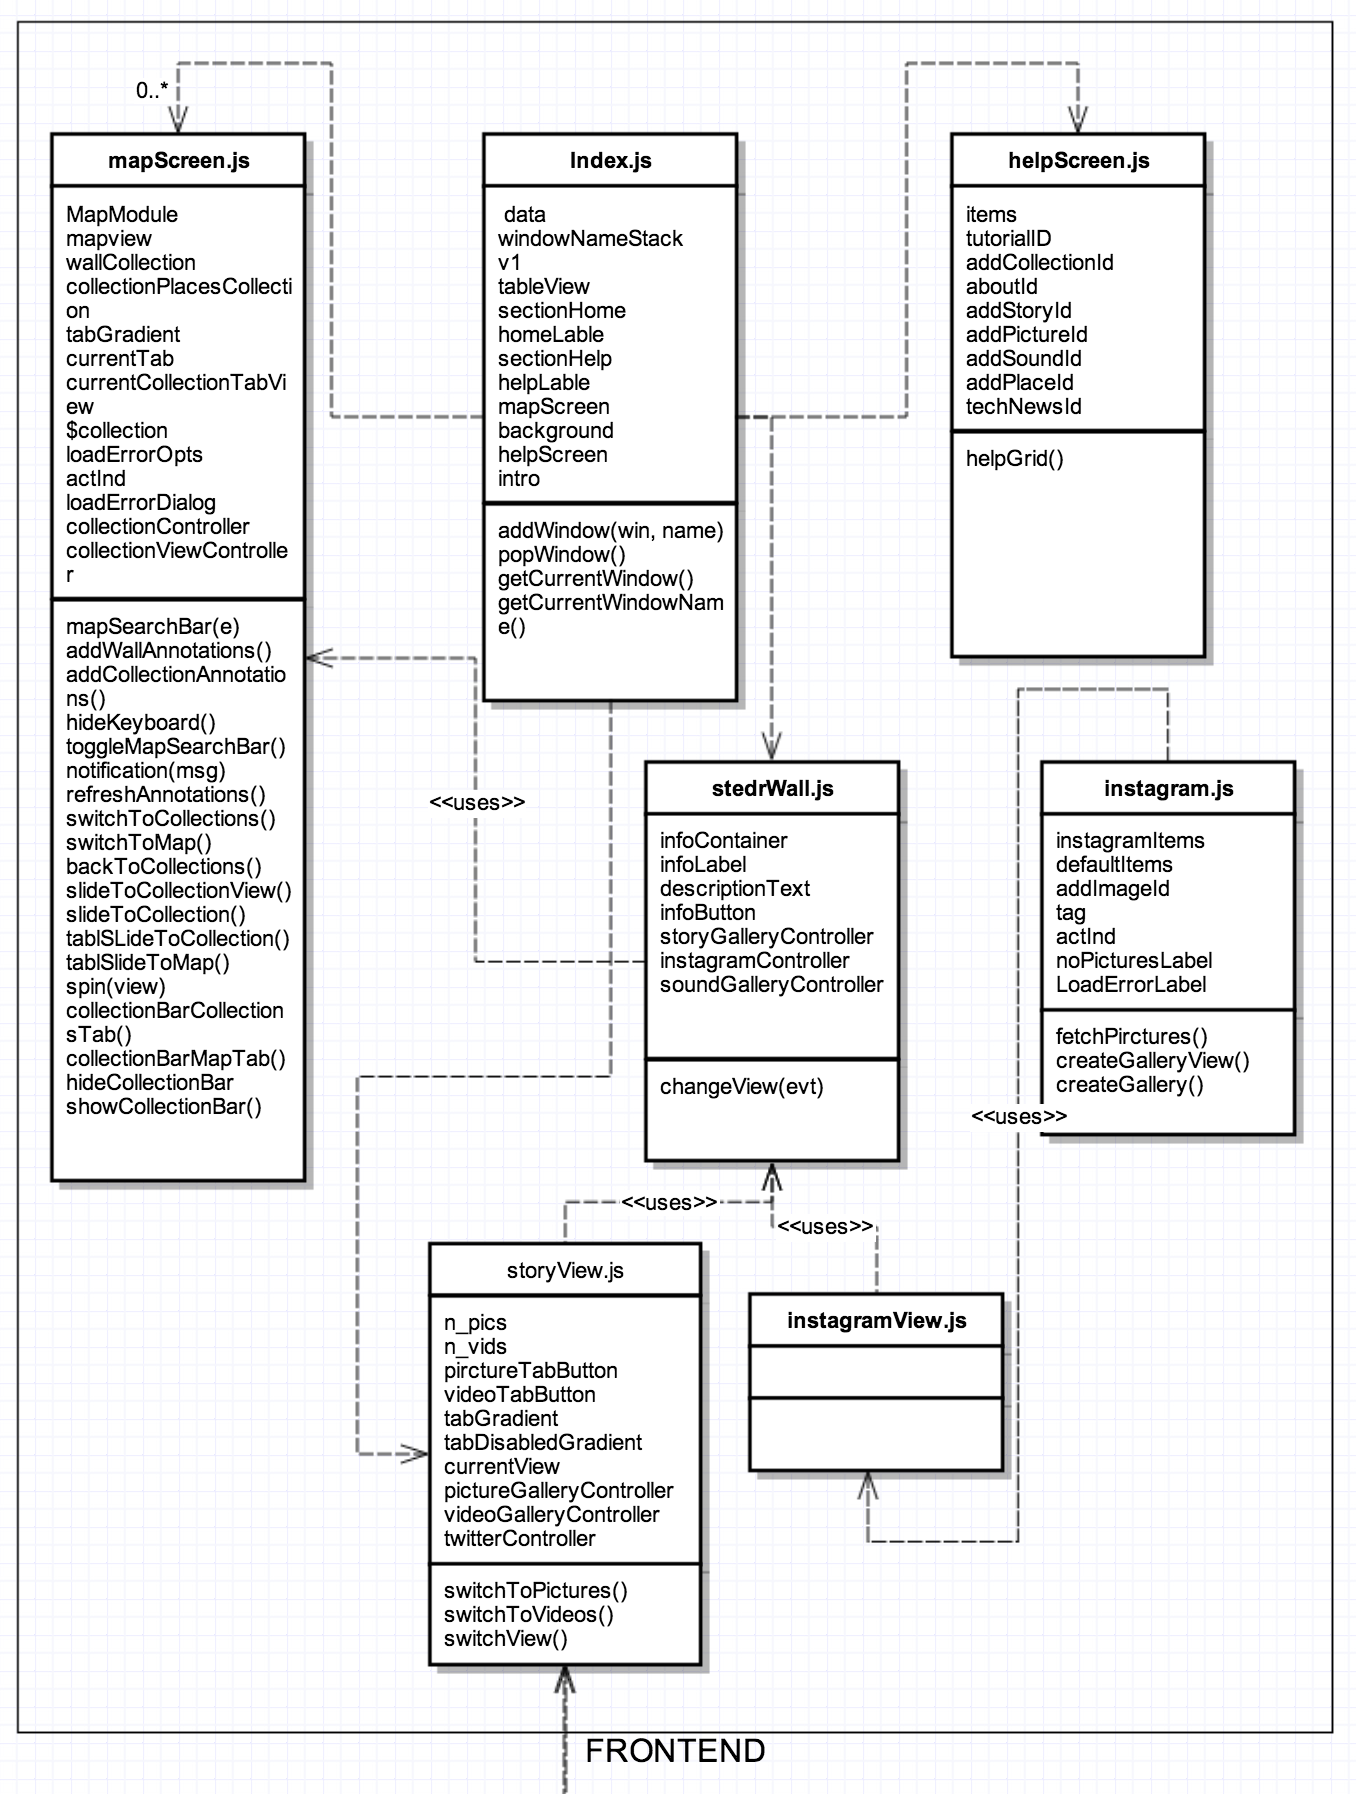
\includegraphics[width=1 \textwidth] {classFront1.png}
\caption{Class diagram for front-end part 1}
\end{figure}

\begin{figure}[!h]
\centering
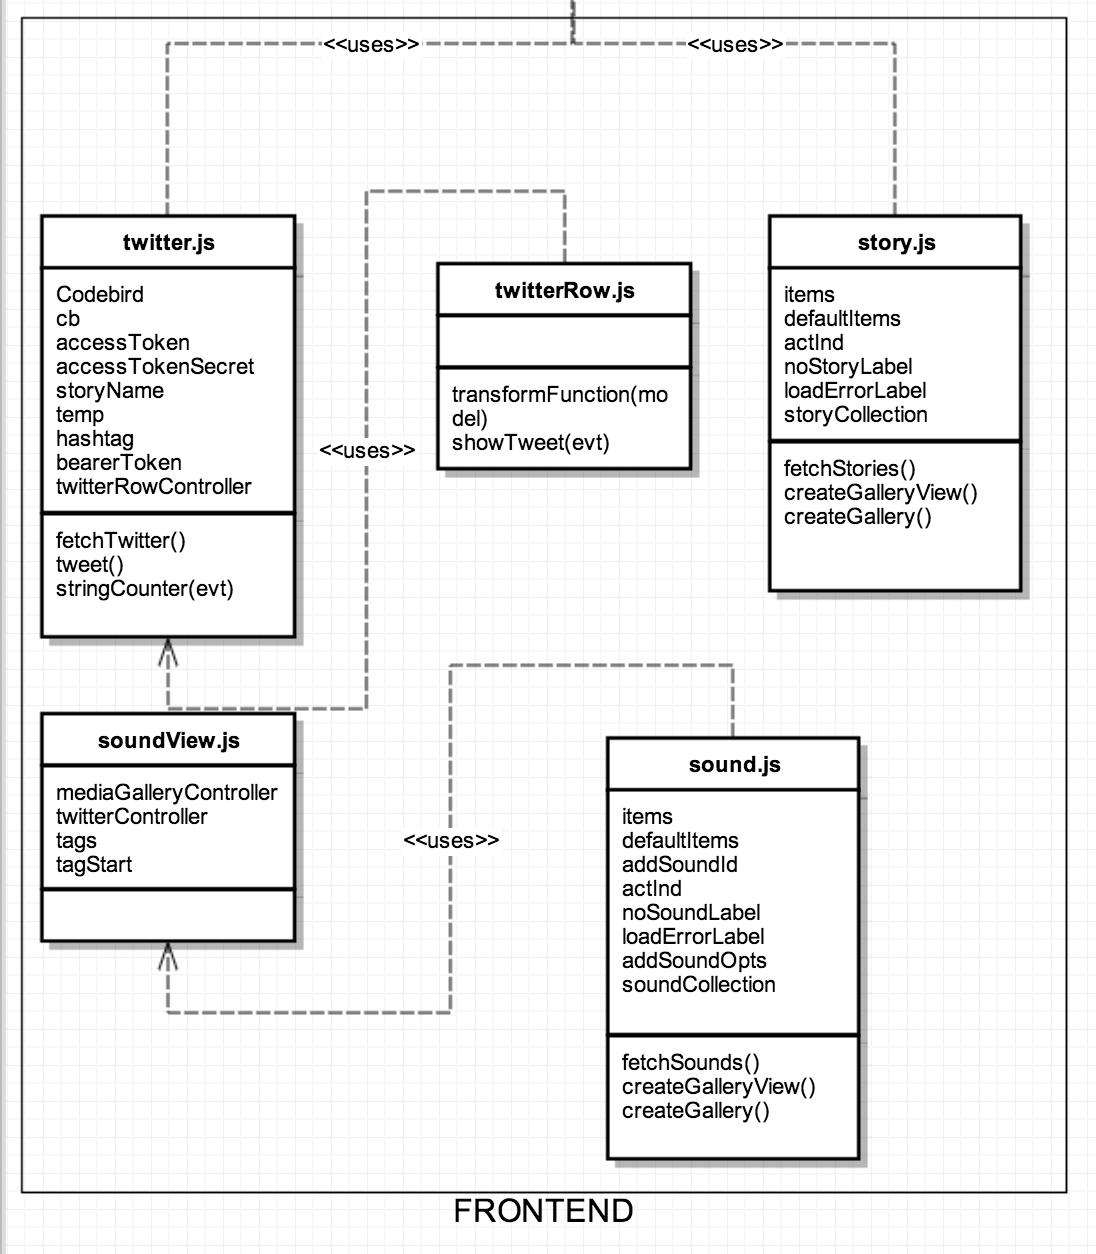
\includegraphics[width=1 \textwidth] {classFront2.png}
\caption{Class diagram for front-end part 2}
\end{figure}

\begin{figure}[!h]
\centering
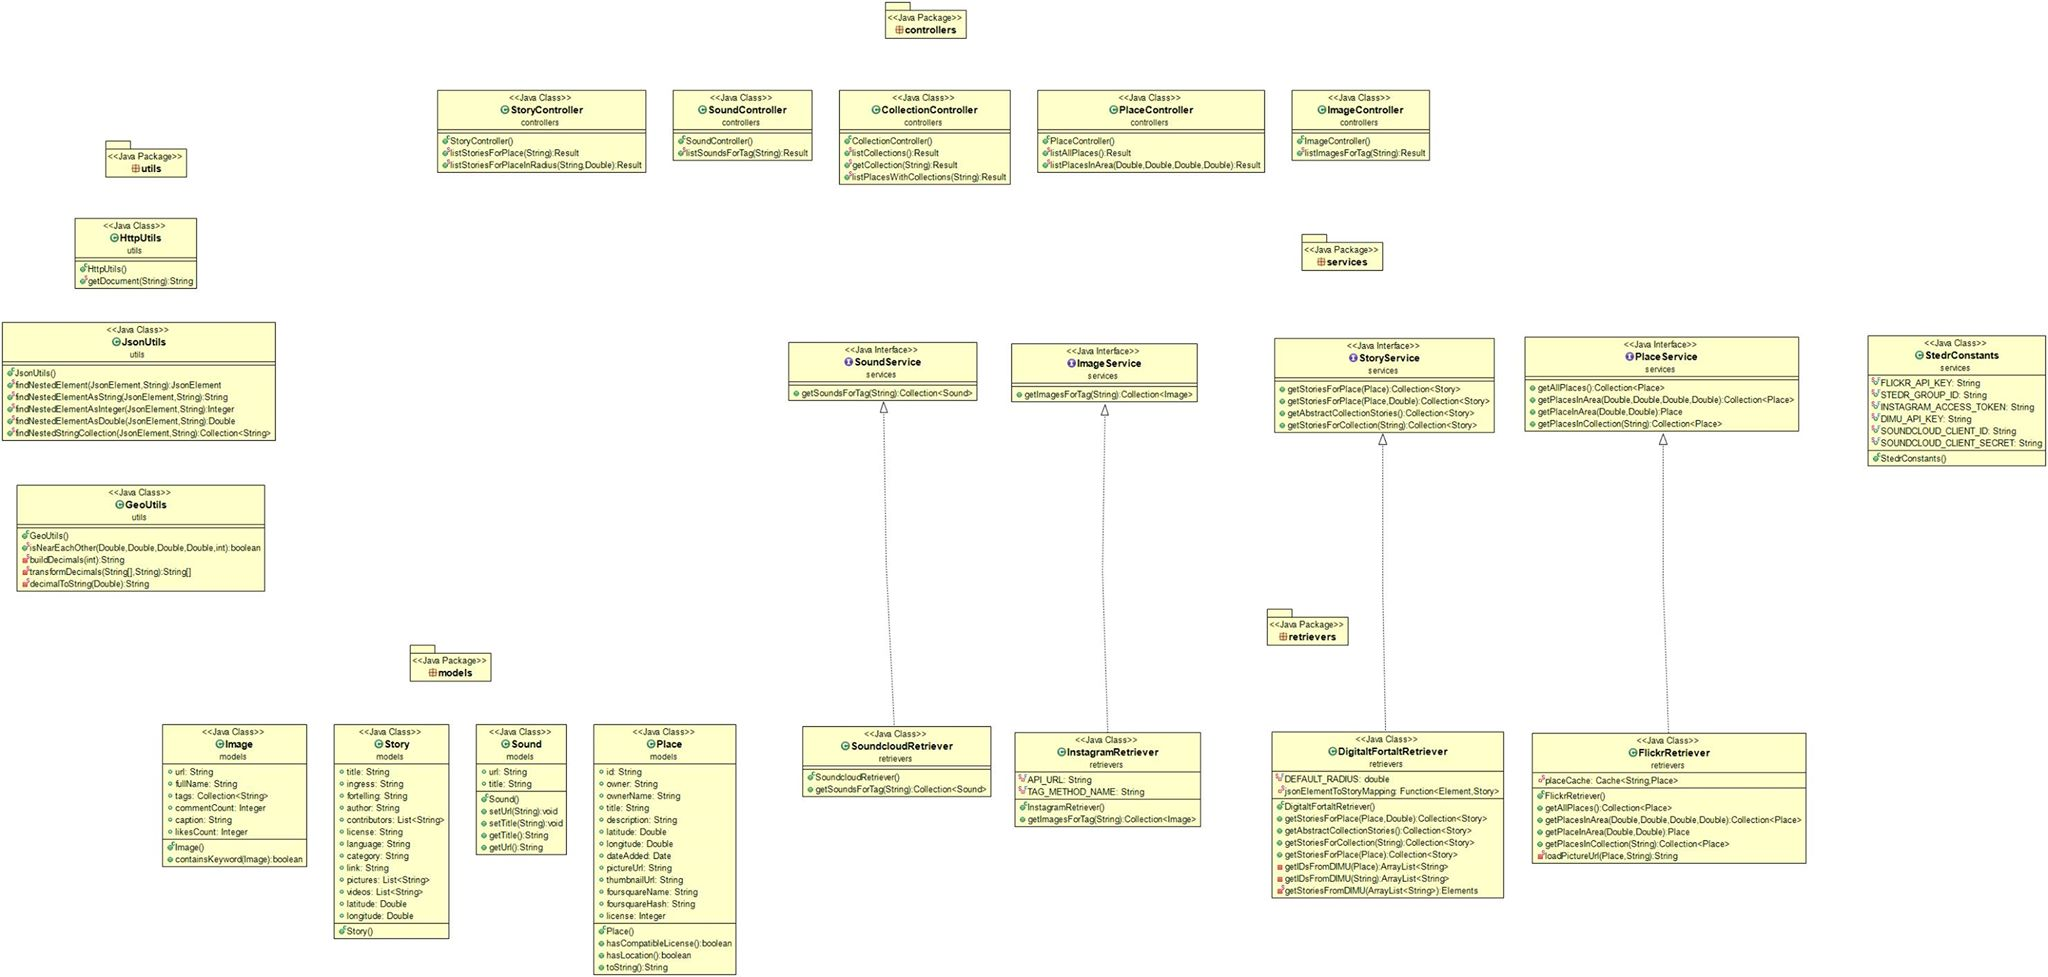
\includegraphics[width=1.3\textwidth, angle=270] {classBack.jpg}
\caption{Class diagram for back-end}
\end{figure}
\clearpage

\subsection{Screenshots}

\begin{center}
\begin{tabular}{cc}
	 	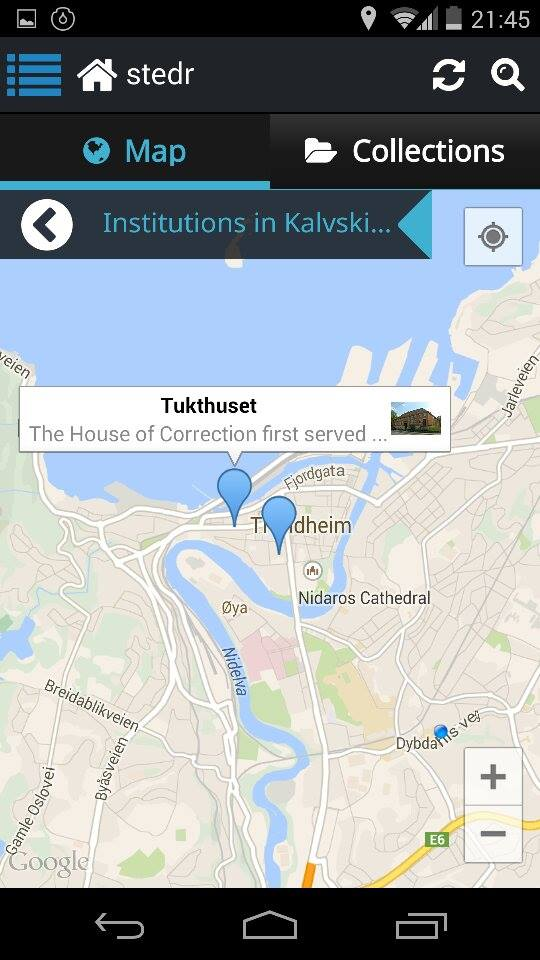
\includegraphics[width=0.35 \textwidth]{res/ScreenShot1.jpg}	& 	
	 	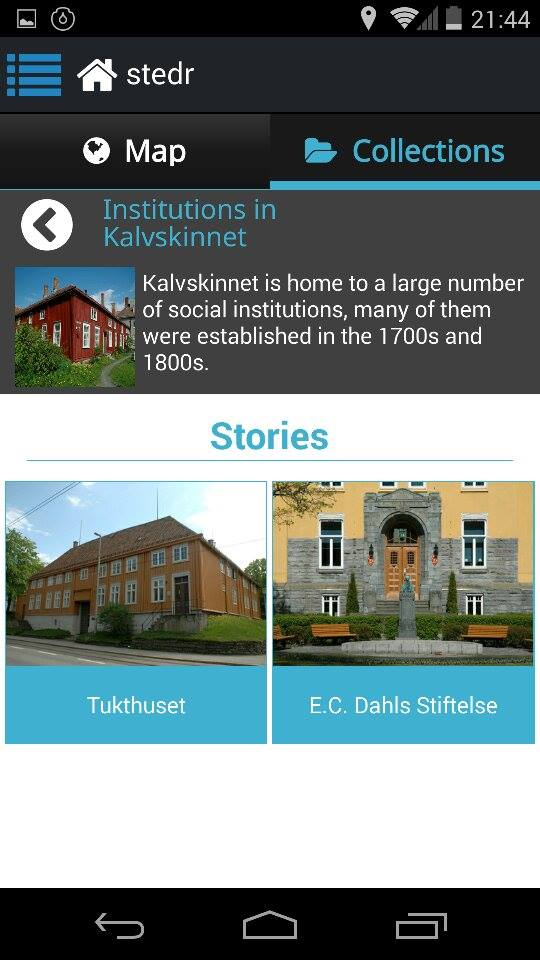
\includegraphics[width=0.35 \textwidth]{res/ScreenShot2.jpg}\\
	 	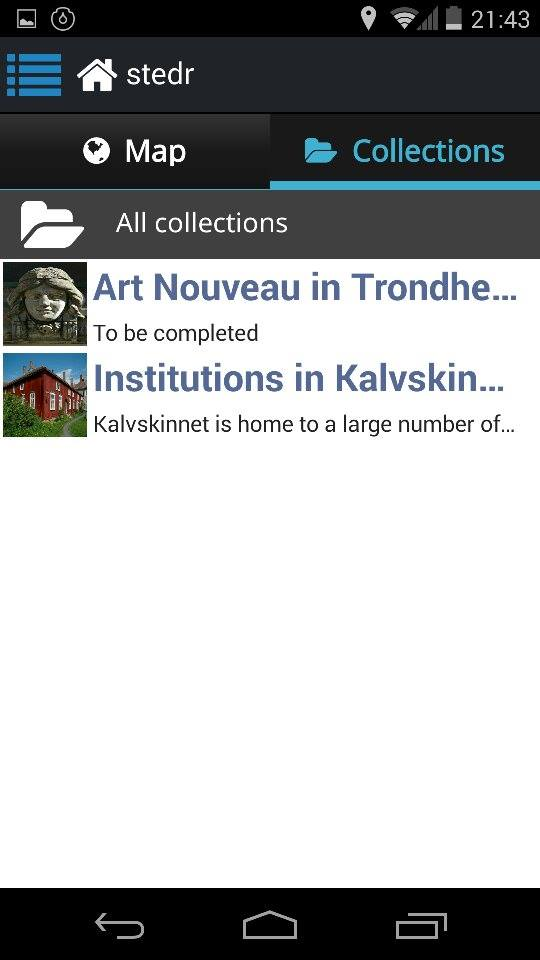
\includegraphics[width=0.35 \textwidth]{res/ScreenShot3.jpg}	&
	 	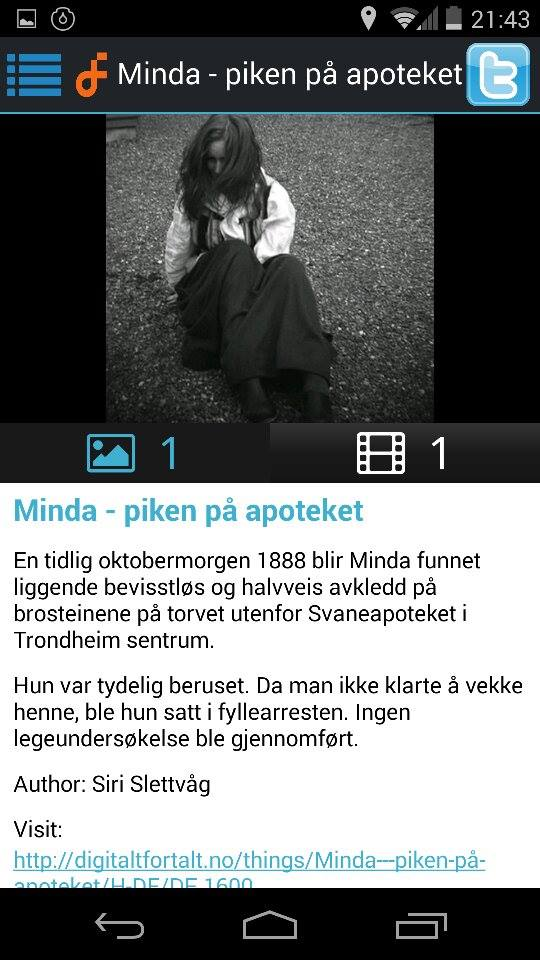
\includegraphics[width=0.35 \textwidth]{res/ScreenShot4.jpg}\\
\end{tabular}
\end{center}

\begin{center}
\begin{tabular}{cc}
	 	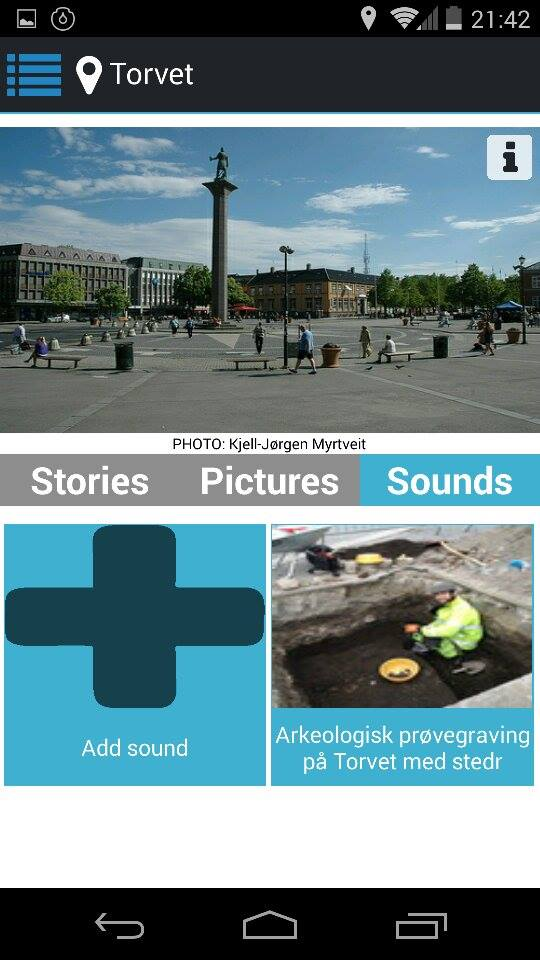
\includegraphics[width=0.35 \textwidth]{res/ScreenShot5.jpg}	& 	
	 	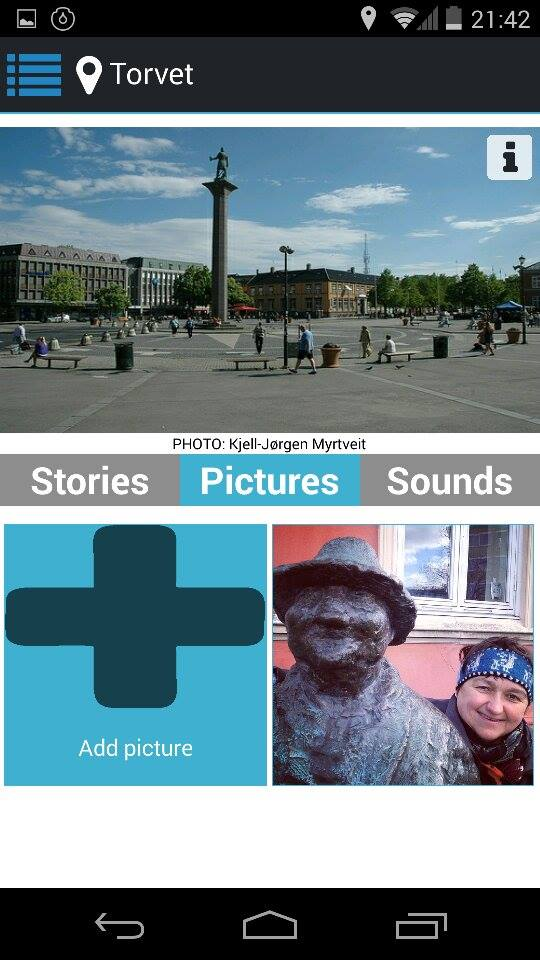
\includegraphics[width=0.35 \textwidth]{res/ScreenShot6.jpg}\\
	 	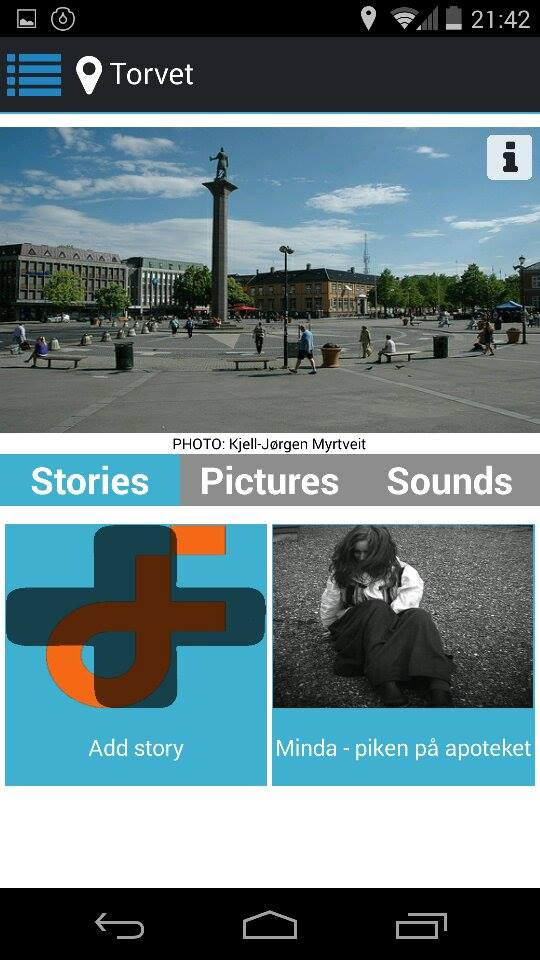
\includegraphics[width=0.35 \textwidth]{res/ScreenShot7.jpg}	&
	 	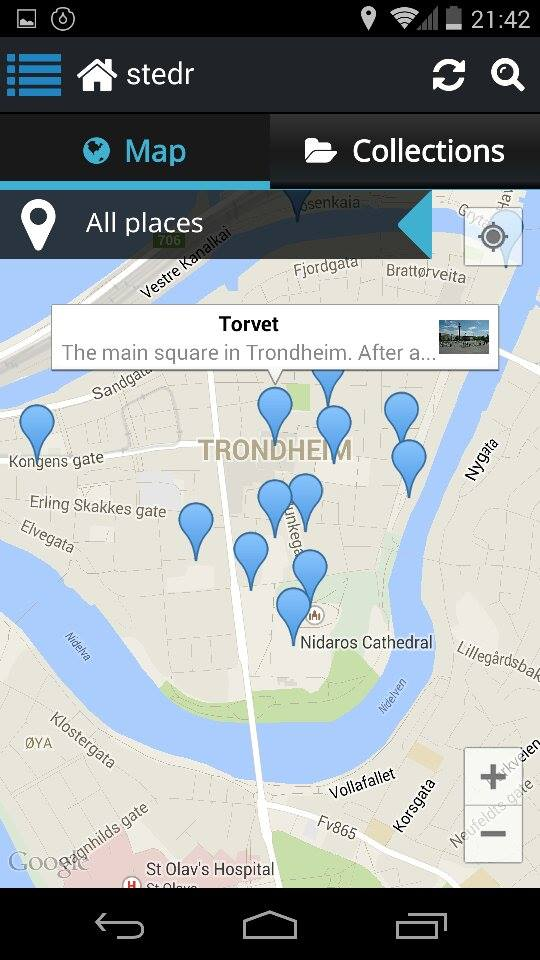
\includegraphics[width=0.35 \textwidth]{res/ScreenShot8.jpg}\\
\end{tabular}
\end{center}

\clearpage

\/*
\thispagestyle{plain}
\printbibheading
\printbibliography[type=book,heading=subbibliography,title={Book Sources}]
\printbibliography[nottype=book,heading=subbibliography,title={Other Sources}]
\clearpage
*/

%Appendices
\newpage
\pagestyle{plain}
\begin{appendices}

%\section{Developers Manual}
%\subsection{Frontend}
%\subsection{Backend}
\section{Developers Guide}
This introductory developers guide, aims to make a developer able to set up Stedr so that the developer gets an overview of how the system works and also how the developer can get started programming. The first part of the guide is about the back-end while the second part is about the front-end. Both of the guides needs to be completed to get the example program running, and the back-end part has to be completed before the front-end part. 

\noindent

This guide is \textbf{not} meant as a tool guide, so some parts of the guide is superficial and it is left to the reader to study the tools closer.

\subsection{Back-end}

The back-end is a Java program using the Play Framework, and the back-end is deployed to the Heroku, a cloud platform hosting applications as services. The source code itself maintained on a GitHub account provided by SINTEF called TagCloud. Before continuing this means that a couple of prerequisites has to be fulfilled by the developer.

\paragraph{The developer should have:}
\begin{itemize}
\item Installed an updated version of JDK 
\item Installed a code editor (Eclipse will be used in the tutorial)
\item A working GitHub-account
\item Installed git
\item Cloned TagCloud/StedR\textunderscore server with the help of Git from GitHub
\item Installed the Typesafe Framework from \href{http://www.playframework.com/download}{Play Framework}
\item An \href{https://www.heroku.com/}{Heroku} account 
\end{itemize}  

On your computer, open up a terminal of your choice (cmd, bash, \dots) and navigate to the folder where you have extracted Typesafe Activator (Play Framework). Depending on your platform type the command which will execute activator. It is possible to use Typesafe Activator with a graphical user interface by passing ui as a parameter. This will look something like:
\begin{center}
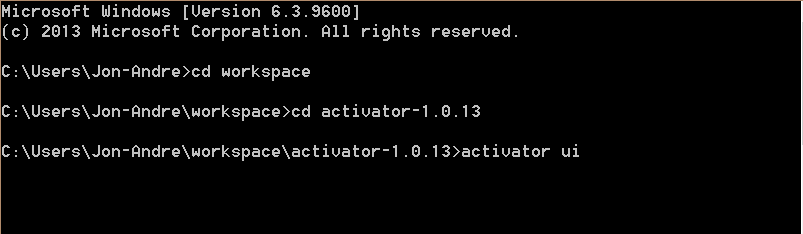
\includegraphics[scale=0.8]{guide/activator1.png} 
\end{center}
The graphical user interface should then open automatically in a browser view. If this doesn't happen check the terminal for error messages.

\paragraph{}
In the right sidebar navigate to the folder where you have cloned StedR\_server from GitHub. Click choose. Now the program is starting to compile, and the server will try to run as a local instance on \href{http://127.0.0.1:9000}{localhost port 9000}. 
\begin{center}
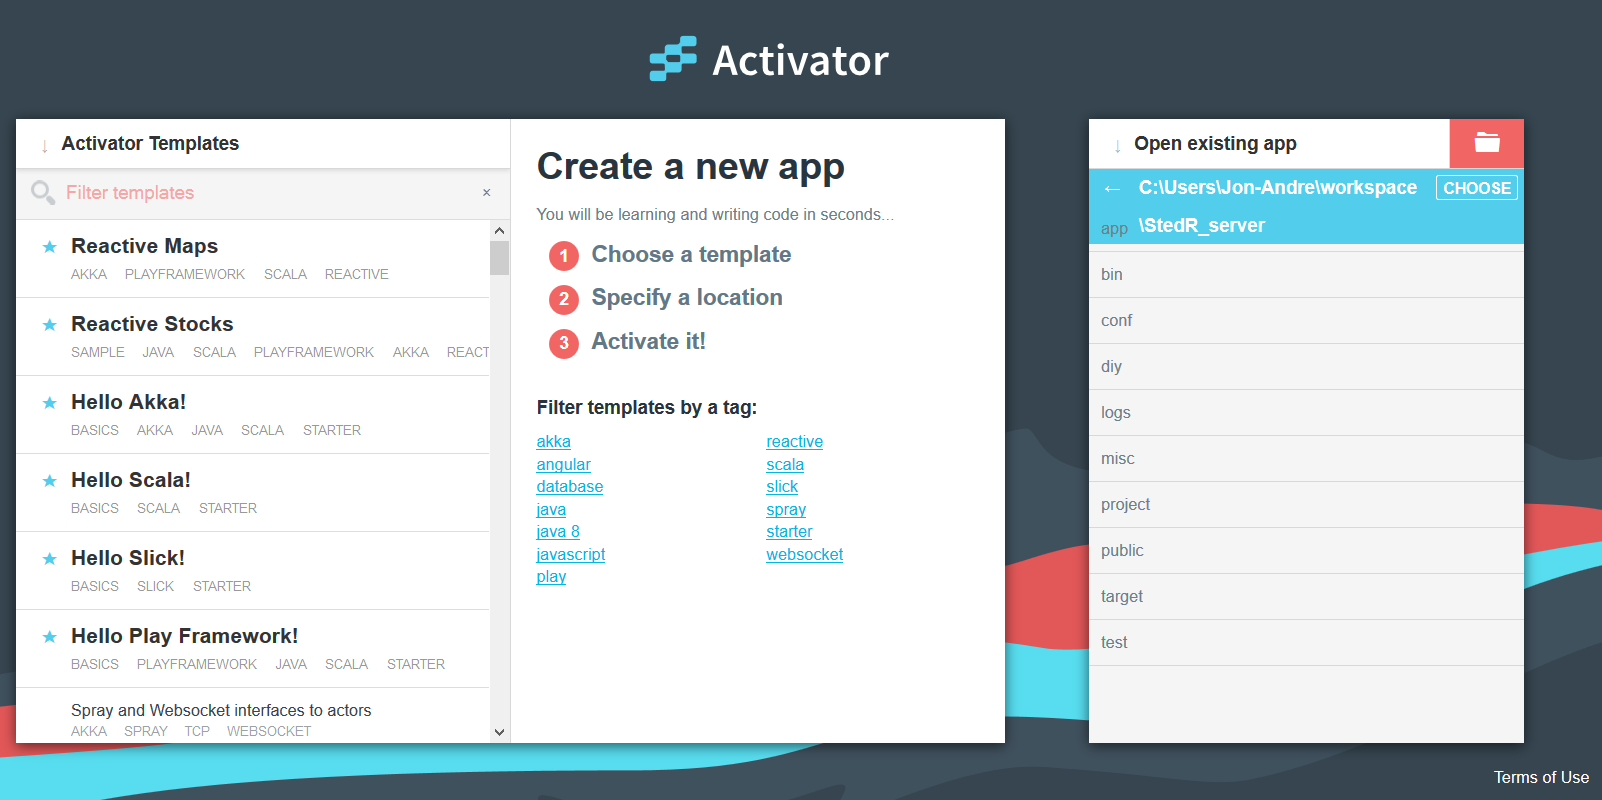
\includegraphics[scale=0.4]{guide/activator2.png} 
\end{center}

Notice that Typesafe Activator itself is running on port 8888. During the compiling of the system problems may occur. Often this is related to a mismatch between Typesafe and Java, for example an updated version of Java and an outdated version of Typesafe often leads to issues. If the program is compiled successfully, something like this should appear at localhost: 

\begin{center}
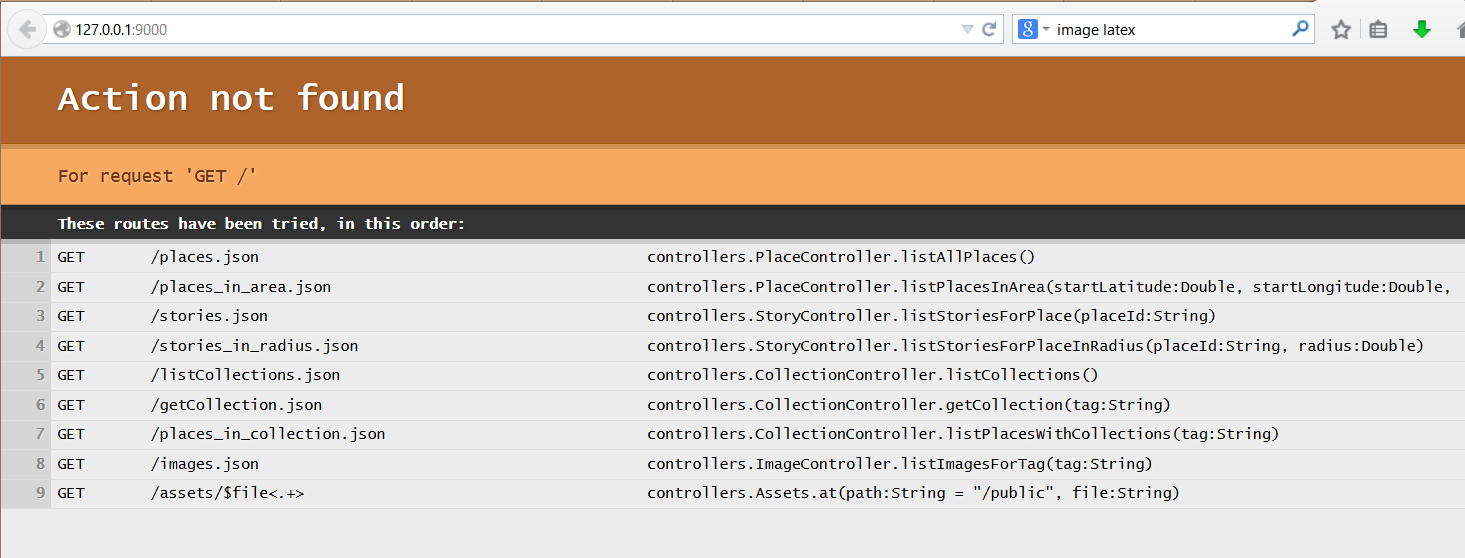
\includegraphics[scale=0.5]{guide/activator3.png} 
\end{center}

If you already have tried importing the folder with the source code to an editor like Eclipse, you may have noticed a lot of errors appears. To import the program and its dependencies as a project: In the left sidebar of Typesafe, click on Code, then the gear-icon. Here you can choose between IntelliJ and Eclipse, and Typesafe will then generate project files and guide you through how to open the program as a project. 
\begin{center}
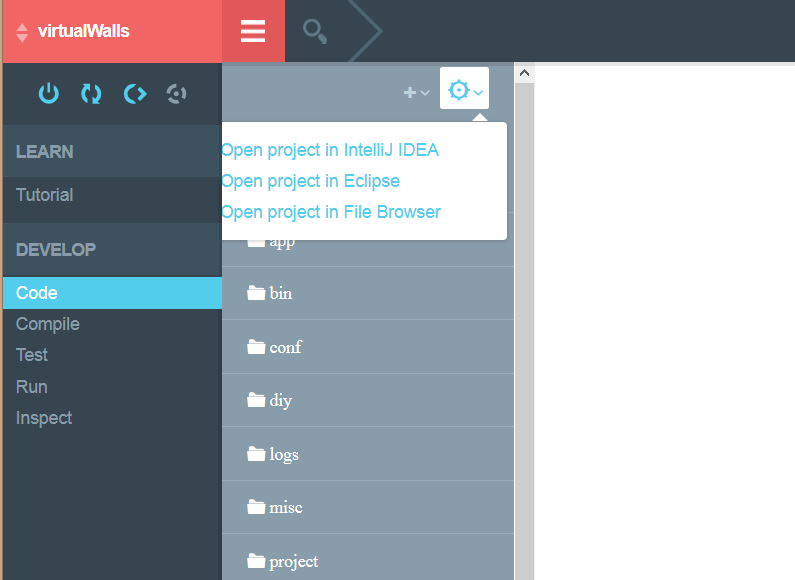
\includegraphics[scale=0.6]{guide/activator4.png} 
\end{center}
Now you should have a running instance of the server locally, and you're also ready to code. 

\paragraph{}

In Eclipse you will get an overview of the different source files and source packages. In the \texttt{Controllers} package you will find \texttt{controllers} that take care of identifying queries (sent as an URL), creating \texttt{Retrievers} that process the queries and at last returning a response to the query. All of the  \texttt{Controllers} are written by former Stedr-developers, but all of the  \texttt{Controllers} extends a  \texttt{Controller} from the Play Framework.

\begin{center}
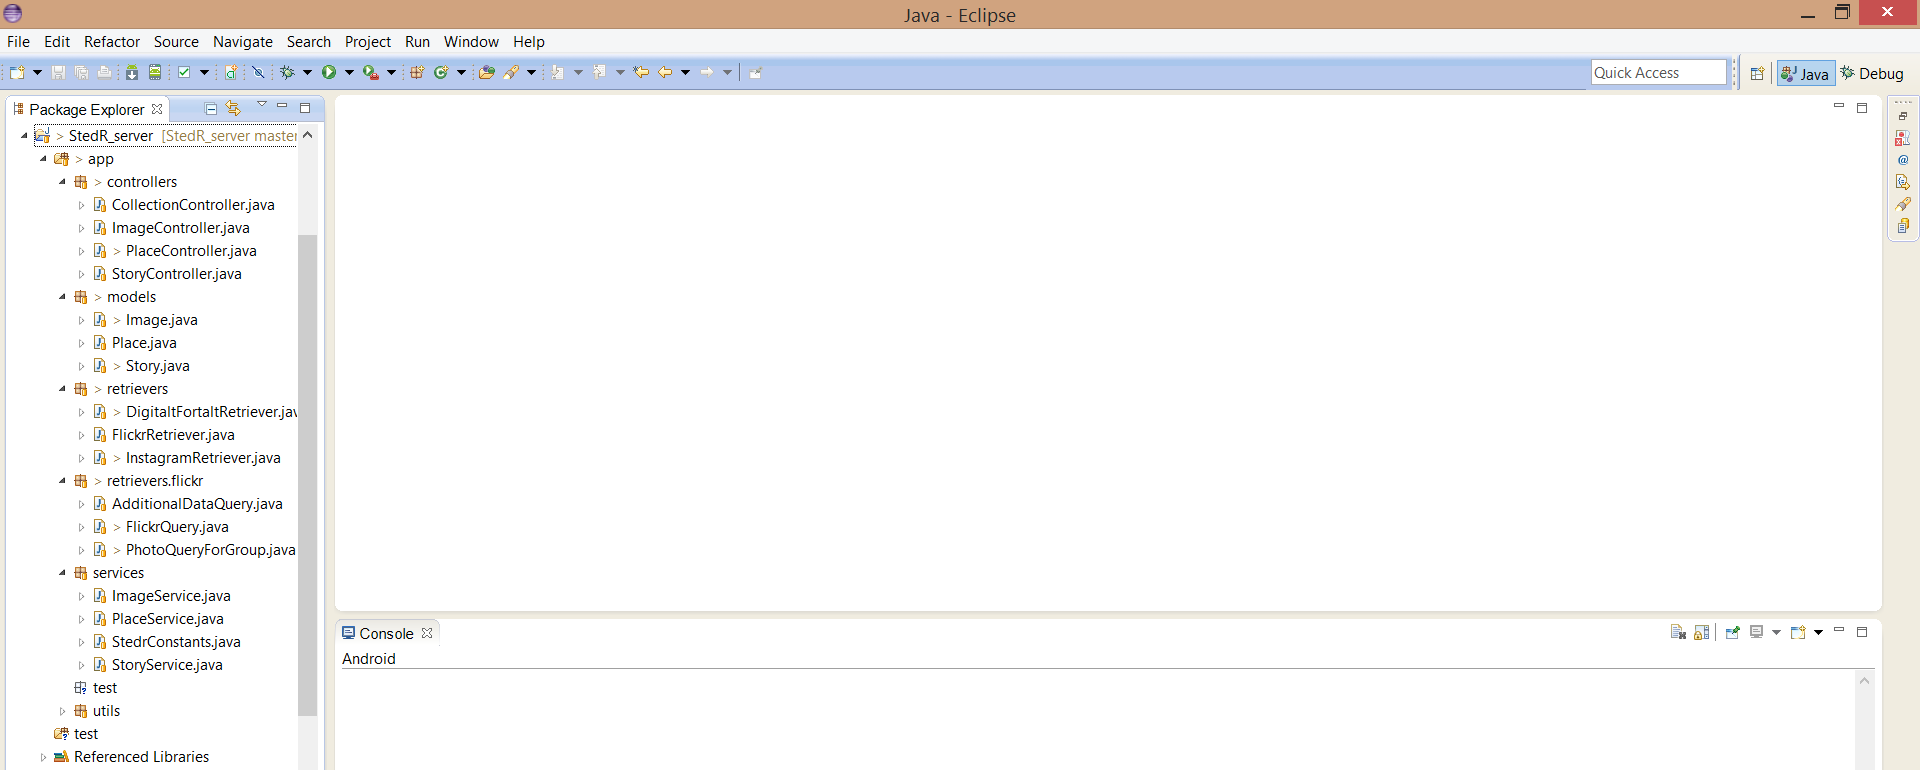
\includegraphics[scale=0.4]{guide/eclipse1.png} 
\end{center}

Now, let's create a controller for our example application:


\begin{center}
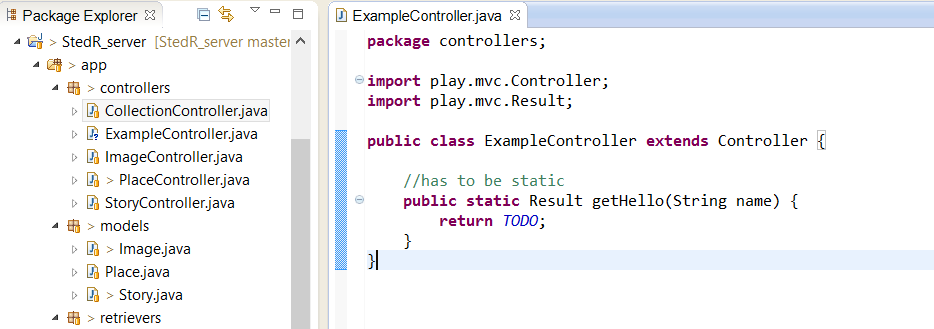
\includegraphics[scale=0.7]{guide/eclipse2.png} 
\end{center}

We ask for a parameter called \texttt{name} which naturally is the name you want to be displayed in the smartphone-application. To pass a parameter you have to edit the file called \texttt{routes} in the conf-folder, the passing is done directly from the smartphone application.

\begin{center}
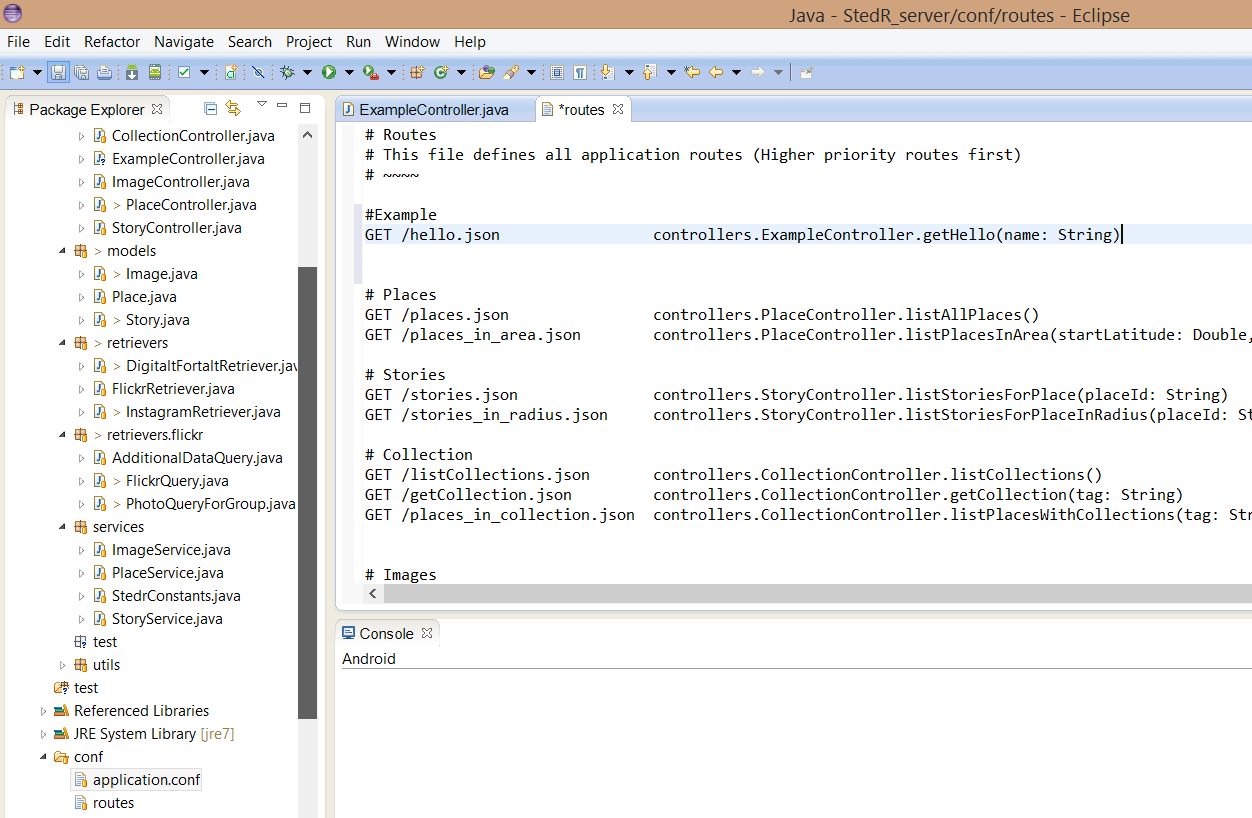
\includegraphics[scale=0.5]{guide/eclipse3.png} 
\end{center}

It would now have been possible to create a \texttt{retriever} directly, but we won't do that. In the services folder there are three files ending with  \texttt{Service.java}. These files are interfaces, and the reasoning behind them is that it should be easy to add or change services. As of now stories are provided by Digitalt Fortalt, so we have a \texttt{DigitaltFortaltRetriever.java} which implements \texttt{StoryService.java} That way we can change the content provider to Wikipedia by creating a new retriever \texttt{WikipediaRetriever.java} which implements \texttt{StoryRetriever.java} A lot of code would then have to be written in order to get the fictional \texttt{WikipediaRetrever.java} functional. Back to the example we will therefore create an ExampleService. 

\begin{center}
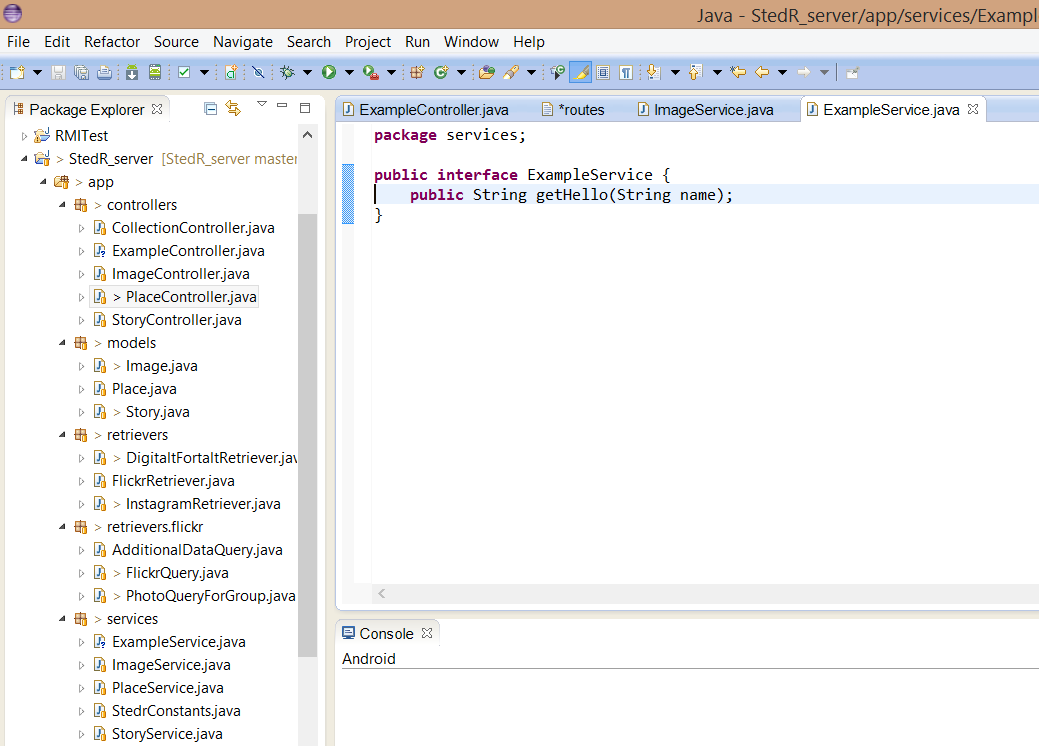
\includegraphics[scale=0.7]{guide/eclipse4.png} 
\end{center}

Now we're ready to implement the \texttt{HelloRetriever.java}

\begin{center}
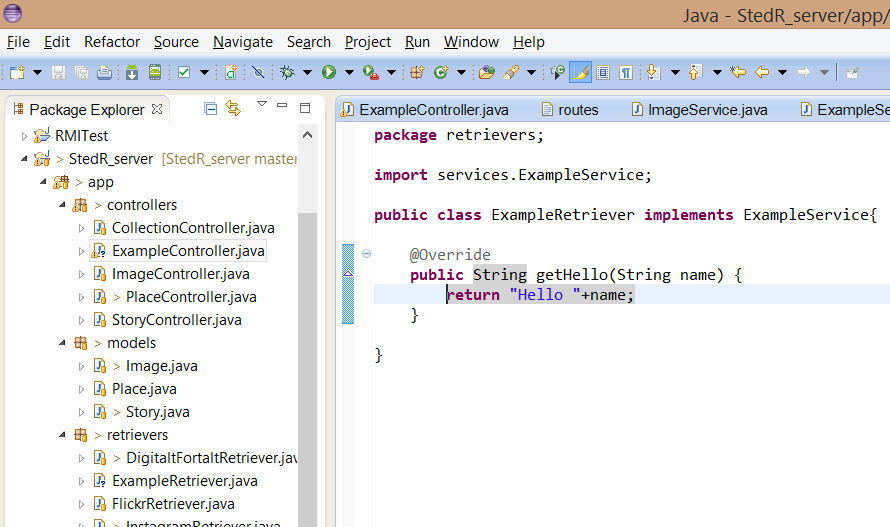
\includegraphics[scale=0.7]{guide/eclipse5.png} 
\end{center}

After the \texttt{HelloRetriever.java} the last thing that needs to be completed is the ExampleController which was created in the beginning of the example

\begin{center}
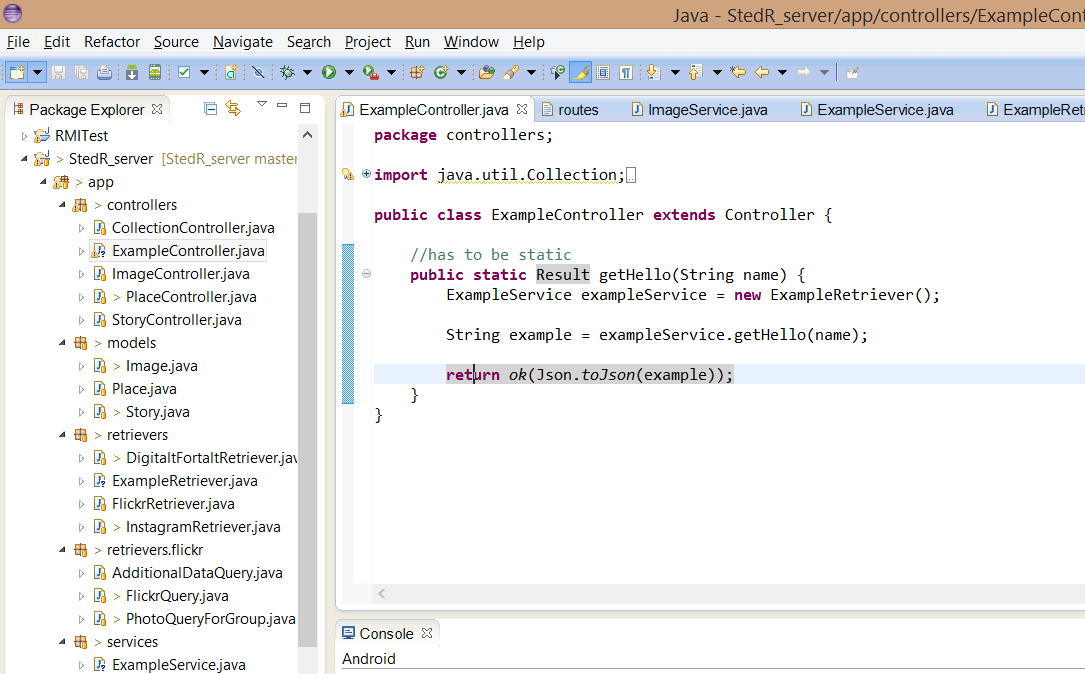
\includegraphics[scale=0.6]{guide/eclipse6.png} 
\end{center}

This concludes in a server which will respond with \texttt{Hello World} if  \texttt{World} is passed as a parameter. To see this, the system has to be recompiled in TypeSafe Activator. After recompiling open \href{http://127.0.0.1:9000}{localhost port 9000}, there you should see:

\begin{center}
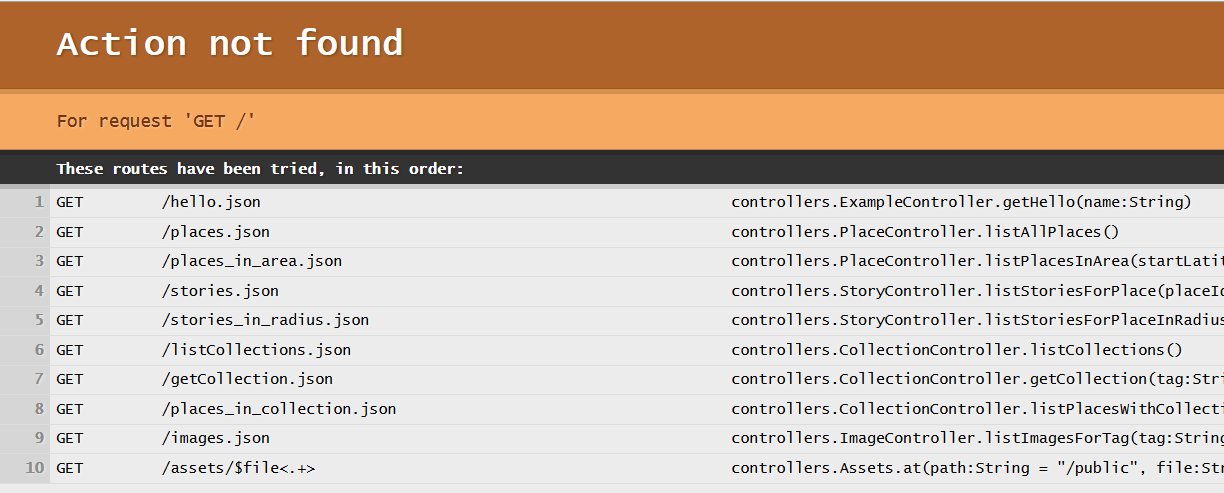
\includegraphics[scale=0.6]{guide/localhost.png} 
\end{center}

If this is correct,  \href{http://127.0.0.1:9000/hello.json?name=world}{http://127.0.0.1:9000/hello.json?name=world} should give:

\begin{center}
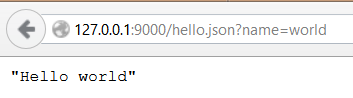
\includegraphics[scale=0.8]{guide/completed.png} 
\end{center}

Normally you would commit this to the git-repository on GitHub, and if the new functionality is to be a part of the running server it should also be commited or deployed to Heroku. This is done by pushing the server commit to \texttt{git@heroku.com:stedr-beta.git}. Note that in order to push to the server directly, you will need contributor access to stedr-beta.herokuapp.com. If this isn't available or provided upon request you can create a new Heroku instance, but then the request URL destinations have to be changed in the smartphone application.

Note that the first server commit to a new Heroku instance is so slow that you can get an error message regarding time-out when compiling. At the time of writing we are not sure if this error is ours or Herokus, because it may seem like the error is related to Herokus slug compiler. Heroku needs to install OpenJDK on their instance the first time the server is pushed to Heroku, OpenJDK is fairly large so this would also explain that the server's slug is fairly large. The error was fixed by adding a \texttt{system.properties}-file under app in the project folder, with the value \texttt{java.runtime.version=1.7}. This file should now be pulled from GitHub when cloning the project.

\textbf{Remember to add the API-keys to the \texttt{StedrConstants.java}. These must ONLY be added to private repositories, and should really only be added to a deployment branch of the project. Also, since almost all of them are owned by members of former dev-teams they may become invalid without notice}:


\texttt{// this apikey belongs to: chrisfro@stud.ntnu.no} \\
\texttt{public static final String FLICKR\_API\_KEY = } \\
\hspace*{4em}\texttt{"cd04f142470e7de7c992b3a3b140f636";} \\
\texttt{public static final String STEDR\_GROUP\_ID =} \\ 
\hspace*{4em}\texttt{"2297124\%40N25"; // escaped} \\
\texttt{this access token belongs to: knut.nerga@gmail.com} \\
\texttt{public static final String INSTAGRAM\_ACCESS\_TOKEN =} \\ 
\hspace*{4em}\texttt{"623771306.1fb234f.09aa9355cc8e469f8839d18385f719d5";} \\
\texttt{// this access token belongs to: Jacqueline Floch} \\
\texttt{public static final String DIMU\_API\_KEY =} \\ 
\hspace*{4em}\texttt{"h\_LUmtZbSAC9CqsDzsuzgg";} \\
\texttt{// these access tokens belongs to: Tor Barstad} \\
\texttt{public static final String SOUNDCLOUD\_CLIENT\_ID =} \\ 
\hspace*{4em}\texttt{"737095f8e223d83af9b88a9b48d90ea9";} \\
\texttt{public static final String SOUNDCLOUD\_CLIENT\_SECRET =} \\ 
\hspace*{4em}\texttt{"c559b568bfa50272ff18bcb27a87fa65";} \\

\subsection{Front-end}

The front-end is developed using Appcelerator Titanium.  Similar to the back-end, the source code itself is maintained on a GitHub account provided by SINTEF called TagCloud. Before continuing this means that a couple of prerequisites has to be fulfilled by the developer.

\paragraph{The developer should have:}
\begin{itemize}
\item A working GitHub-account 
\item A working Appcelerator-account 
\item Installed git
\item Cloned TagCloud/VirtualWall with the help of Git from GitHub.
\item An Android or iOS device
\end{itemize}  

Note that you need a to install the sync software for your device and make sure you have USB debugging enabled. It is also important to note that you need a Mac in order to build the program for iOS devices. Android or iOS device is not required, since it is possible to use an emulator. 

\paragraph{}

Download \href{http://www.appcelerator.com/titanium/}{Appcelerator Titanium}.

Install titanium by following the installation wizard. When titanium is finished installing, open it. Titanium will ask you to choose a workspace location, where your projects will be stored. You then have to log in with your Appcelerator-account.

Titanium will then most likely attempt to install software development kit (SDK) for Android. If it does not, you can do so via the dashboard. Click the “Get Started” tab and scroll to “Configure Native SDKs”, click Android SDK and make sure it is updated. The Tizen and Blackberry development kits are not necessary for this application.

If you have a Mac, you should be able to install the iOS SDK as well. You need this if you are testing the application on an iOS device.

\begin{center}
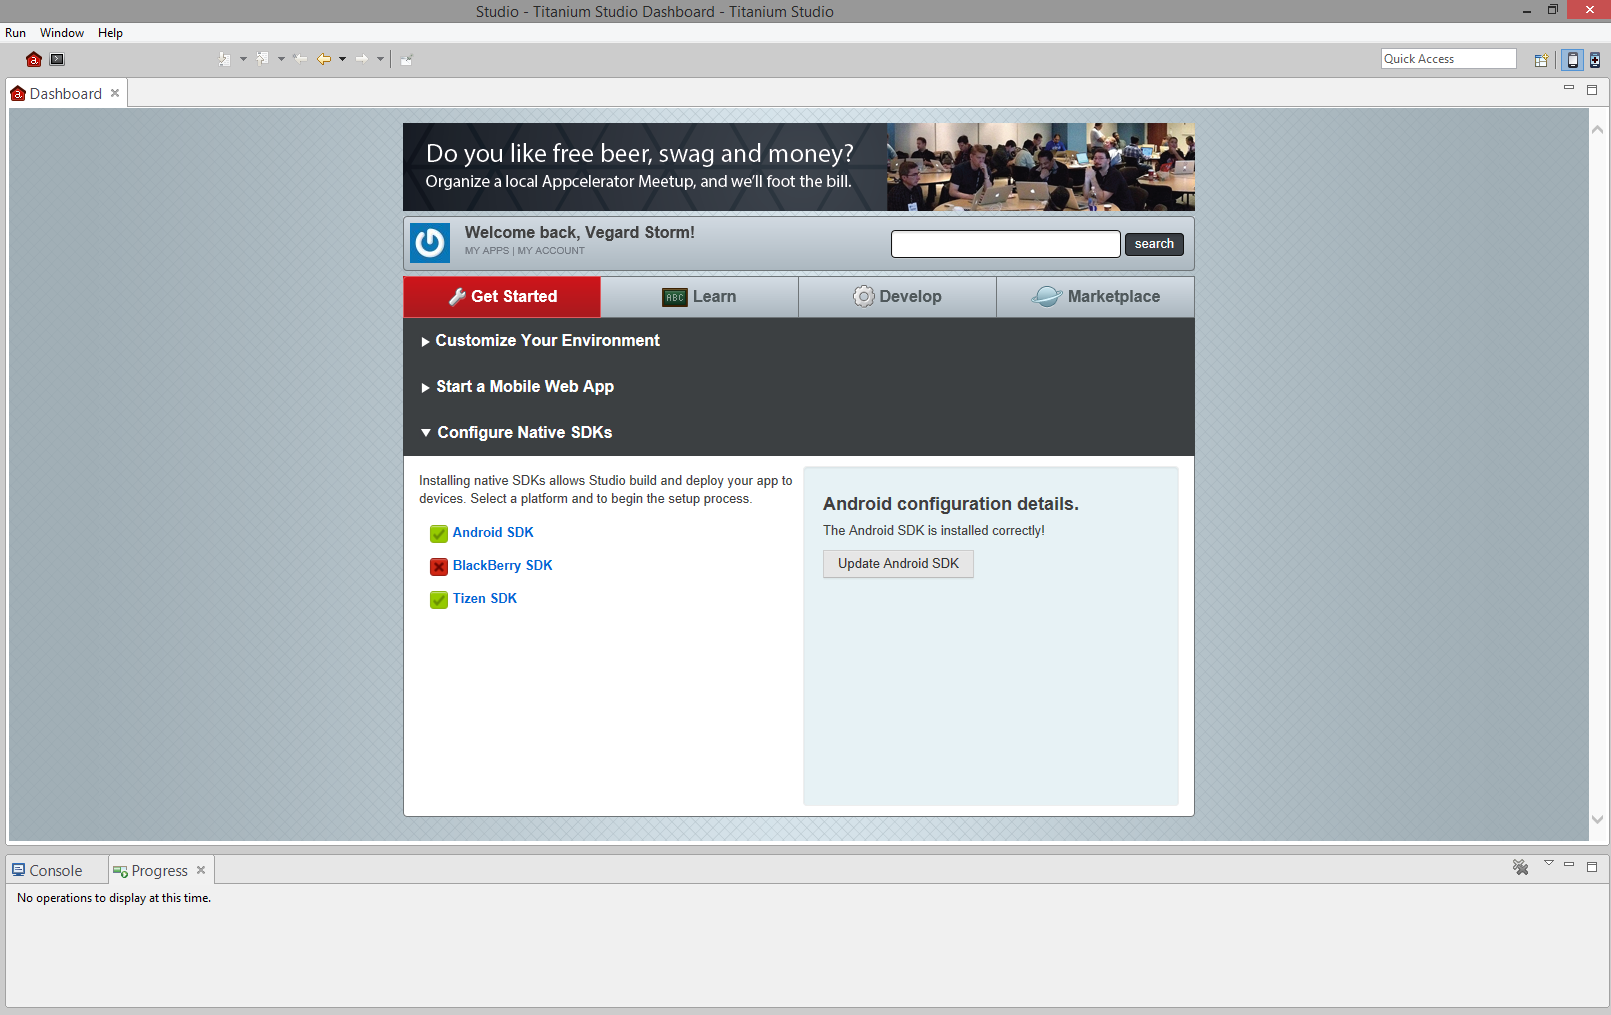
\includegraphics[scale=0.3]{guide/f1.png} 
\end{center}

Now we are ready to import the Stedr project.
1. Right click in the project explorer and choose “Import”.
2. Choose the “Existing Folder as New Project”-option under “General” and press “Next”.

\begin{center}
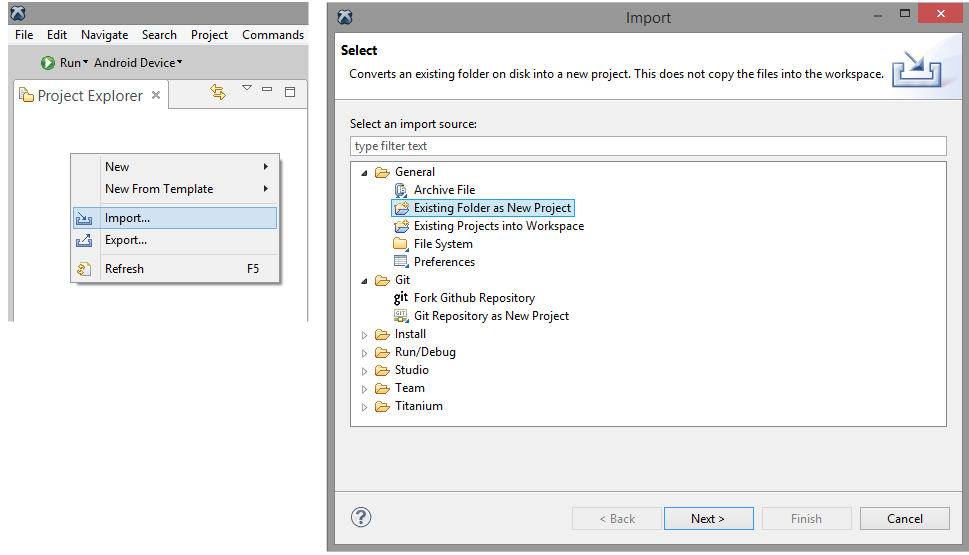
\includegraphics[scale=0.45]{guide/f2.png} 
\end{center}

3. Click browse and choose the folder where you downloaded Stedr and press “OK”. 
Example: C:/Users/Vegard/Documents/GitHub/VirtualWall/stedr
4. Under “Project type” make sure Alloy is checked as primary and mobile is checked (This should happen automatically) and press “Finish” if everything is in order.

\begin{center}
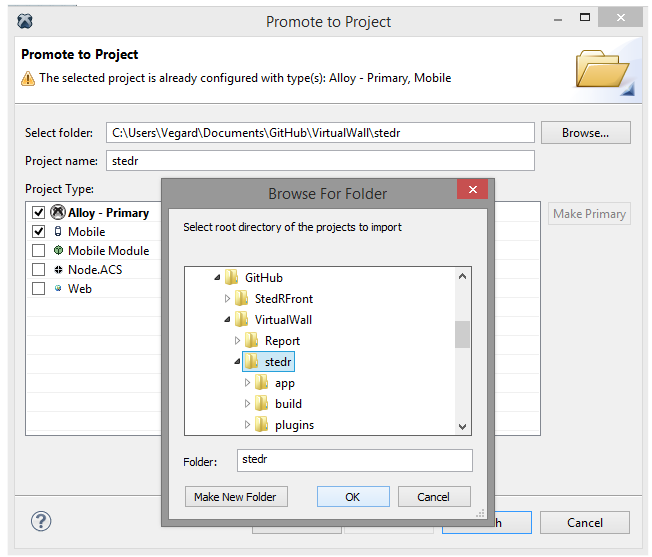
\includegraphics[scale=0.45]{guide/f3.png} 
\end{center}

We are now ready to code or run the project. It might beneficial to try to run the program on your device or an emulator before you start coding. If you have already done what is explained in the prerequisites and connected your device to the PC via USB, your phone should show up in the list of devices as displayed below. If it does, select it and click “Run”. However if it does not, make sure you have the synchronization software for your device installed, and that you have “USB debugging” enabled in your phone settings. If you have issues finding the “USB debugging” option on your phone, it may be because you do not have access to developer settings. The easiest way to figure out how to get access is to google “how to access developer options on *your device*“.

\begin{center}
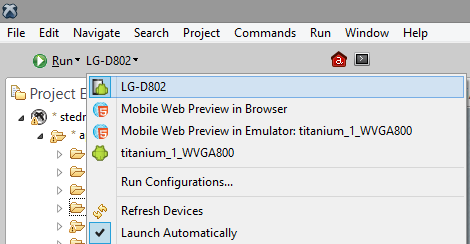
\includegraphics[scale=0.45]{guide/f4.png} 
\end{center}

\paragraph{Emulator:}
It is possible to run the program on the official Android emulator, but it has some performance issues. An alternative emulator is the \href{https://shop.genymotion.com/index.php?controller=order-opc}{Genymotion}. Note that this emulator has some restrictions when asking for a free license, so make sure not to break their term of service. 

Genymotion does not support Google Apps (i.e Google Map Service) which is needed to run stedr. To install Google Apps on Genymotion, see this \href{https://www.youtube.com/watch?v=iCRNqCXGNK0}{screencast}. Before continuing it is also practical to add adb to the environmental path, so that adb is accessible directly in the terminal. On Windows you can locate adb.exe under the folder platform-tools where you have installed the Android SDK. 

With Genymotion started (the emulated device should be running) enter \texttt{adb install -r stedr.apk}. It is easiest to do this from the builder folder where, but you can probably send the location of the apk as a parameter. Notice the -r parameter, this is for reinstalling an apk which becomes necessary to use if the apk already is installed at the emulated device.

\begin{center}
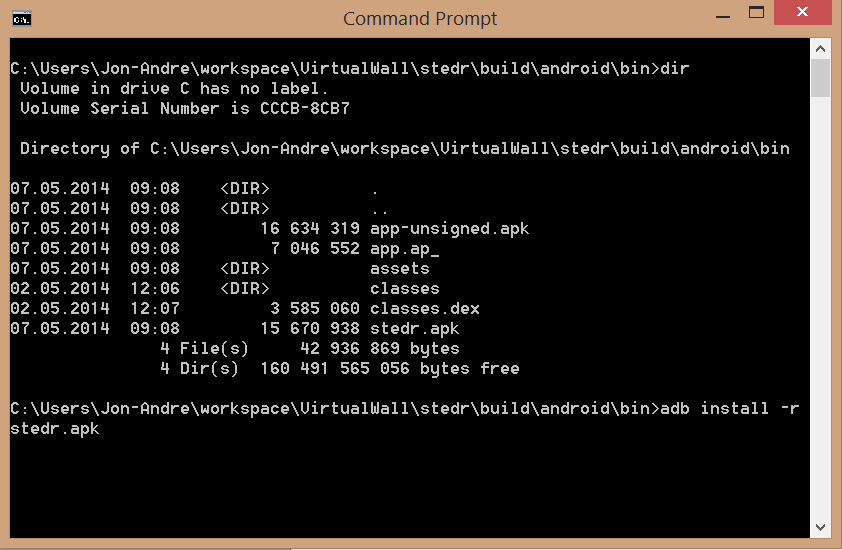
\includegraphics[scale=0.7]{guide/f45.png} 
\end{center}
\clearpage
\paragraph{Structure in Titanium alloy:}
if you explore your newly added Stedr project in the project explorer you will notice that under the app folder there are a number of subfolders.

\begin{wrapfigure}{l}{0.5\textwidth}
\begin{center}
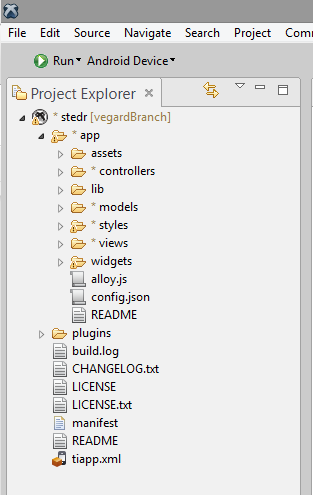
\includegraphics[scale=0.45]{guide/f5.png} 
\end{center}
\end{wrapfigure}

The views-, styles- and controllers-folders are the ones you will be working with the most.

Views:
This folder contains an XML-file for every view and the basic structure of it containing different UI-elements. Each element with an “id” will also get the properties assigned to it in the corresponding styles-file and controller-file.

Styles:
This is a folder of TSS-files that are used to design elements used in the corresponding XML-file based on “id”.

Controllers:
This folder is where the JavaScript classes for the different views are stored and where you can add code that affect the corresponding view. You add new UI elements,  event listeners, functions and more to achieve the desired functionality and design.


Additionally we have the assets folder, where media like pictures are stored; the lib folder, where you store relevant imported libraries; the models folder, where you can create models that are useful when for instance converting a string into an object; the widgets folder, where imported pre-made UI-elements are stored.


\paragraph{Coding Example}
In this example we assume that you have completed the back-end example and uploaded it to the server stedr-beta.herokuapp.com.

We will be creating a view that contains a label with the value that we retrieve from the server stedr-beta.herokuapp.com/hello.json?name=world. If done right, the text “Hello World” should be displayed on the screen when opening this view. 

1. Begin by creating a new devTest.xml-file in the “views”-folder, a devTest.tss-file in the “styles”-folder and a devTest.js-file in the “controllers”-folder.

\begin{center}
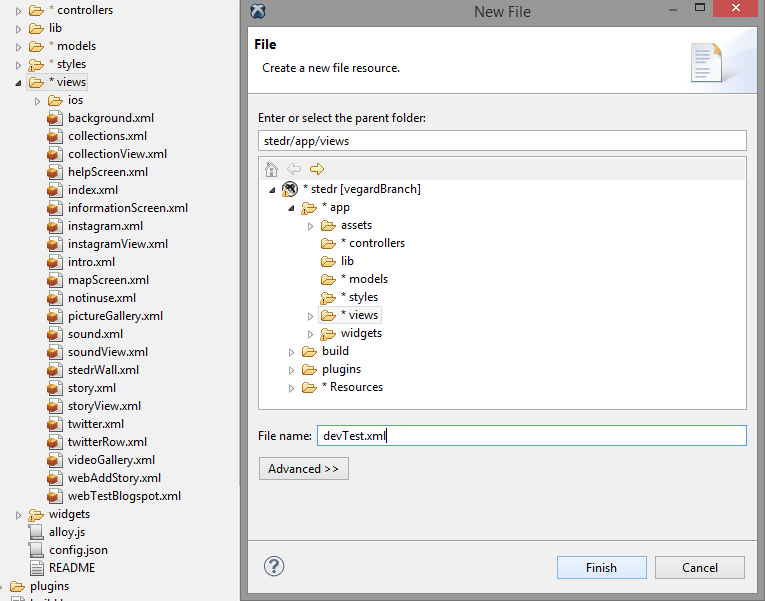
\includegraphics[scale=0.45]{guide/f6.png} 
\end{center}

2. Creating the XML-file for the view. This is the basic structure of the UI elements. You can also add some properties to the different elements.

\begin{center}
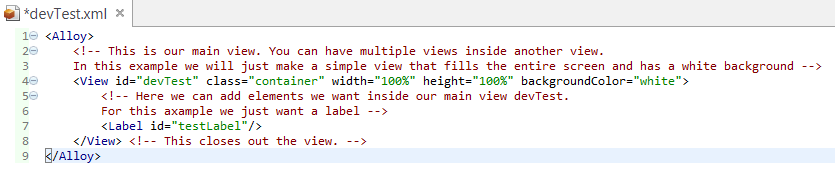
\includegraphics[scale=0.45]{guide/f7.png} 
\end{center}

2. Creating the TSS-file for the view. The purpose of this file is mainly to stylize UI-elements that are used more than once in the XML-file. Even though a TSS-file is not necessary for a simple view like is this and can be done easily in either the XML- or the JavaScript-file example, here is how you would stylize the label using TSS: 

\begin{center}
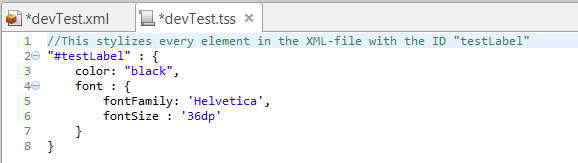
\includegraphics[scale=0.45]{guide/f8.png} 
\end{center}

3. Creating the JavaScript-file. This is where we retrieve the information from the server, as well as set the text of the label.

\begin{center}
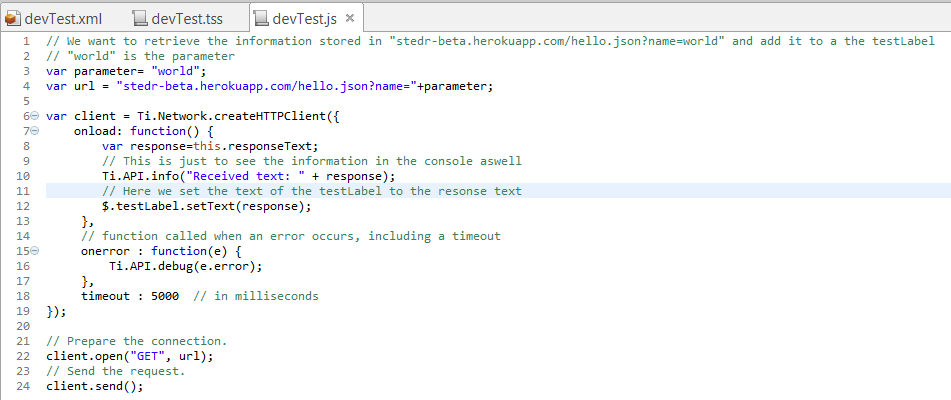
\includegraphics[scale=0.45]{guide/f9.png} 
\end{center}

Now all we have to do is open this view where we want it. For test purposes i will in this example set it to open automatically when you open the app. To do this, we have to go into the index.js file under controllers. Every window/view opens or closes through this class because this is where the window stack is. To make sure the test view is shown automatically, scroll down to the bottom of index.js and add it right above \$.index.open() as shown below:

\begin{center}
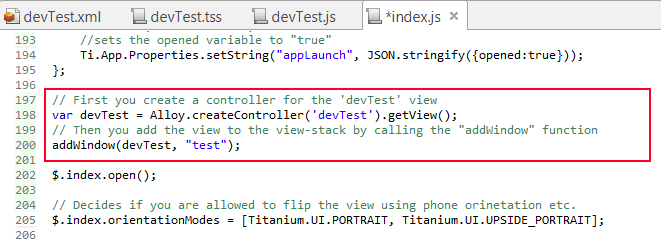
\includegraphics[scale=0.45]{guide/f10.png} 
\end{center}
Now if you save and run you should see something like this when you start the application on your phone:

\begin{wrapfigure}{l}{0.5\textwidth}
\begin{center}
\includegraphics[scale=0.10]{guide/f11.png} 
\end{center}
\end{wrapfigure}


We have now gone over the basics of how to create a view as well as retrieving information from the server. To further understand how to develop Stedr using Titanium, looking at and understanding the previous code is essential. The documentation available on the \href{http://docs.appcelerator.com/titanium/3.0/}{Appcelerator website} is also extremely helpful when learning about Titanium:



\section{Status Report Example}
\subsection{Status Report}
%--------------Status report-------------

\newpage
\thispagestyle{plain}
\begin{tikzpicture}[remember picture, overlay]
	\draw[line width = 1pt] ($(current page.north west) + (0.5in,-0.5in)$) rectangle ($(current page.south east) + (-0.5in,0.5in)$);
\end{tikzpicture}

SINTEF\\
\begin{centering}
Storytelling\\
\huge{Summary Status Report}\\
\end{centering}

\vspace{1cm}
\textbf{1. Introduction}\\

The last week has been pretty busy with a lot of progress in terms of development. The last customer meeting turned out to be very constructive and the customer seemed to be satisfied with the recent development of the system.\\[6pt]

\textbf{2. Progress summary}\\

\href{https://docs.google.com/spreadsheet/ccc?key=0Aigjd3Z4fa8YdGhtR0tqN0d4Q19TR0FmQ2pTVTR1X1E&usp=drive_web#gid=0}{Updated Activity Plan (8)}

\href{https://docs.google.com/spreadsheet/ccc?key=0AlhGbQmvU9bddHl2VWVjWHhiX3VMREc0NWY4UE5hd3c&usp=sharing}{Milestone/Gantt}\\[6pt]

\textbf{3. Open / Closed problems}\\

The last week has almost been problem free, and the progress has been pretty good. Regarding the continued development there has been a delay, because of some content which have not been made available to the group from the customer.\\

In the following week it will be difficult to keep up the momentum from last week, as Easter is approaching (unavailability because of travelling) and a couple of the group members are in China for a school excursion. The group members that still are available will therefore focus on few assignments which they are familiar with from earlier.\\[6pt]

\textbf{4. Planned work for next period}\\

\href{https://docs.google.com/spreadsheet/ccc?key=0AqgF_sCiXohadDQ4SlZKTTZ1ZWZ6djF2dllaZGRPSGc&usp=drive_web#gid=0}{New Activity Plan (9)}

\textbf{5. Updated risk analysis}\\

\href{https://docs.google.com/spreadsheet/ccc?key=0AlhGbQmvU9bddGs0M0tBd3ZaNUxvMnBaQnNLb0FoWnc&usp=drive_web#gid=0}{Risk analysis}

\clearpage

%-------------------------------------------
\subsection{Activity Plan}
\includepdf[pages={1}, angle=270]{res/ActivityPlan_VI_Updated.pdf}
\subsection{Risk Analysis}
\includepdf[pages={1,2,3}]{res/Risk_analysis.pdf}


\section{Meeting Example}

\subsection{Group Meeting}
Here follows an example of notes one of our meetings. The summarys from the meetings are written in norwegian, and translating them for the report was not something we prioritized.\\

\clearpage
\begin{tikzpicture}[remember picture, overlay]
	\draw[line width = 1pt] ($(current page.north west) + (0.5in,-0.5in)$) rectangle ($(current page.south east) + (-0.5in,0.5in)$);
\end{tikzpicture}

Til stede: Alle

\textbf{Agenda:}
\begin{itemize}
\item Oppsumering fra forrige gang
\item Gjort siden sist
\item Evaluering av stedr
\item Preliminary report
\item Diverse
\item Til neste gang
\end{itemize}

\textbf{Oppsummering fra forrige gang:}\\
Forrige gang ble vi enige om å i hovedsak se nærmere på ‘stedr’ og evaluere appen. Siden sist har vi også hatt møte med supervisor og Sintef, det foreligger ikke noe referat fra Sintef-møtet enda. På grunn av sykdom var dette møtet med Babak og ikke den opprinnelige kunden Jacqueline.  

\textbf{Gjort siden sist:}\\
Øyvind: Mock-up, og alt fra lista.\\
Hallvard: Titanium, APIer, RISK.  \\
Jon-Andre: Titanium og oppsett mot stedr, skrevet en liten evaluering av stedr, agilefant, PHP/symfony, jobbet litt (for lite) på RISK-dokumentet.  \\
Tor: Mange oppgaver viste seg overflødige, kommer tilbake\\
Vegard: Titanium, LaTeX, sharedLaTeX.\\
Jørgen: God evaluering av stedr, RISK\\

\textbf{Evaluering av stedr:}
Diverse UI-bugs. F. eks kan man ikke rotere telefonen. Ikke noen scroll-funksjon på ‘pictures’. I overkant mye scroll enkelte steder, man kan scrolle forbi slutten av teksten. Twitter tillater ikke mer enn 140 ord, men det gjør appen. Er det noe poeng å tweete fra stedr, eller skal man bare hente inn? Jørgen har prøvd å få inn et bilde fra instagram, men dette dukker ikke opp i stedr etter 12 timer.
Måten stedr henter inn historier (vha. hashtags) gjør at det blir mye irrelevant informasjon. Autensisering opp mot Twitter er rart, hva er stedr homepage. Vi liker mye av designet. Hva er identiteten/poenget til appen? For utdypninger se eget dokument.\\

\textbf{Preliminary report:}\\
Risk-list er nesten ferdig. Jørgen, Jon og Øyvind skal møtes på lørdag for å jobbe og fullføre midterm.\\


\textbf{Diverse:}\\
For nå tar vi det med ro i LaTeX, bruker Google Docs i første omgang. Tor og Hallvard har sett litt på skytjenester (sky-backend), noe som kan virke interessant. \\

\begin{tikzpicture}[remember picture, overlay]
	\draw[line width = 1pt] ($(current page.north west) + (0.5in,-0.5in)$) rectangle ($(current page.south east) + (-0.5in,0.5in)$);
\end{tikzpicture}

\textbf{Til neste gang:}\\
Øyvind: Prelim-rapport, fikse kodekopier\\
Hallvard: APIer, balsamering\\
Jon-Andre: Prelim-rapport, referat fra Sintef\\
Tor: Se på skybackend\\
Vegard: APIer, prøve å få kildekoden til å fungere i Titanium\\
Jørgen: Prelim-rapport\\

\clearpage


%\includepdf[pages={1,2}]{res/Motereferat_05-02-14.pdf}

\subsection{Customer Meeting}
Here is an example of the summart of a meeting with our customer. Again the text is in norwegian.
\clearpage
\begin{tikzpicture}[remember picture, overlay]
	\draw[line width = 1pt] ($(current page.north west) + (0.5in,-0.5in)$) rectangle ($(current page.south east) + (-0.5in,0.5in)$);
\end{tikzpicture}

\textbf{Videomøte med Jacqueline 19.02.2014}\\

	Til stede fra gruppe: Øyvind, Jørgen og Jon-Andre \\
	Fra kunde: Jacqueline Floch\\

Gruppa har fått mye informasjon, men hva synes Sintef er viktigst? \\
\begin{enumerate}
\item APIet til Digitalt Fortalt
\item Stable bilder til samme sted.
\item Gjøre appen bedre og forbedre integrasjonen mot eksisterende APIer.
\item Skape interesse gjennom sosiale medier (link til fortelling f. eks)
\item Filtrering
\item Koble til andre databaser (Soundcloud)
\end{enumerate}

Vil beholde så mye som mulig av det som allerede finnes i appen. Det ble brukt mye tid på design i høst, så dette bør ikke prioriteres nå.

Filtrering: Når et sted blir hentet kan man f. eks få en liste med tags. Filtrering basert på brukerprofil (og generelt) vil for øyeblikket være litt problematisk grunnet få fortellinger.  

DF har link til Wikipedia.

Hvis vi har forslag til forandring både backend/frontend så kan dette gjennomføres.

Informerer om den lille brukerundersøkelsen vi har hatt, og at vi har et inntrykk av at den sosiale delen. 

Flickr API: Et sted er definert som et bilde, geolokasjon, bilde er delt innenfor en gruppe. Gruppe-APIet til Flickr er ikke optimalt, gruppe er brukt for å gjøre søket enklere. Backend henter alle bilder og informasjon fra den gruppa.

Gruppa har et inntrykk av at appen ved førstegangsbruk er litt vanskelig, kanskje det bør være innlagt en sidemeny.

En litt abstrakt utfordring er: Hva er et sted, og hvor stort er et sted?

\textbf{Notiser:}\\
 	-Det APIet som ble brukt i høst fungerer ikke nå\\
	-Gruppa bør sjekke ut Trondheim Byguide\\

\clearpage

\subsection{Supervisor Meeting}
Here are some notes from one of our meetings with the our supervisor Mohsen Anvaari. 
We found these meetings to be a great resource during our project, giving us constructive criticism and advice. This specific meeting occurred 18.02.2014.

\clearpage
\begin{tikzpicture}[remember picture, overlay]
	\draw[line width = 1pt] ($(current page.north west) + (0.5in,-0.5in)$) rectangle ($(current page.south east) + (-0.5in,0.5in)$);
\end{tikzpicture}

\textbf{Meeting with Supervisor 18.02.2014}\\

He thought the report was generally good, but some small things were missing:

In the introduction we should have given a short introduction to the customer.

He had some issues with the structure of the report:

The term Software Engineering is too broad.
Should rather be split up in sections like Architecture, Design etc. 
An alternative would be to simply split the structure in to Sprint 1, 2 etc.

Time organization should just be called Project Planning.

Never use “things” in the report. Be more specific.

“GUI and APIs” - For what? Specify that we will work on Stedrs GUI and API.

Remember to give an brief description on what the application is for. Explain the usage.

Process is fine.

Timeplan and architecture is fine, but needs to be more detailed for the next version. 

Some of the Non-functional-reqs is functional. ISO standard. Chose 3 or 4. How we tackled it later. Diary is functional.

Linking is superimportant!

Risk analysis is very good.

\clearpage





\section{Other}

\subsection{Mock-ups}
\label{sec:mockups}

In the beginning of the project we did made mockups to describe our ideas and thoughts. These was later dismissed as the project progressed, but we implemented ideas from them later on, so even though they are not directly relevant to the final project, we feel they are relevant enough for the subject, in terms of how time were spent etc, to include them in the report.

\begin{figure}[!h]
\centering
\includegraphics[width=0.9 \textwidth] {res/mockup1.png}
\end{figure}

\begin{figure}[!h]
\centering
\includegraphics[width=0.9 \textwidth] {res/mockup2.png}
\end{figure}

\begin{figure}[!h]
\centering
\includegraphics[width=0.9 \textwidth] {res/mockup3.png}
\end{figure}


\end{appendices}
\end{document}